\documentclass[twoside]{article}
%-------------------------------------------------------
% Do not change anything between these "------"
% However, please contact the managing editor if you need
% any of the packages referenced here.

\pagestyle{myheadings}
\setlength{\oddsidemargin}{44pt}
\setlength{\evensidemargin}{44pt}
\setcounter{page}{1}

\usepackage{url,intmacros,graphicx}
\usepackage{amssymb,amsmath}
\usepackage{capt-of}


\def\BibTeX{{\rm B\kern-.05em{\sc i\kern-.025em b}\kern-.08em
    T\kern-.1667em\lower.7ex\hbox{E}\kern-.125emX}}

\numberwithin{equation}{section}

\newcommand{\email}[1]{\\ \small{\url{#1}} \\}
\newcommand{\institution}[1]{\\ \parbox{3.0in}{\small{#1}}}
\newcommand{\keywords}[1]{\small\textbf{Keywords: }#1}
\newcommand{\AMSsubj}[1]{\noindent\textbf{AMS subject classifications: }#1}
\newcommand\whenaccepted{Submitted: May 20, 2006;
                         Revised: November 10, 2010; July 18, 2011; September 1, 2012; Match 27, 2014; }
\newcommand{\tilt}{\!\!\sim\!\!}
\newcommand{\eqspace}{\;\;\;}


%-------------------------------------------------------


%  You may add additional packages here.  However, if they
%  are not available with the usual LaTeX distribution,
%  they must be supplied with the final, accepted LaTeX.

% Fill in your title here. (Retain the footnote.)
\title{Variance Arithmetic\footnote{\whenaccepted}}

% Delete the "\and" or add more as needed
\author{Chengpu Wang
\institution{40 Grossman Street, Melville, NY 11747, USA}
\email{Chengpu@gmail.com}}

% Put a short running title within the first argument to
% this command.  Do not alter the second argument
\markboth{CP Wang, \textit{Variance Arithmetic}}
         {\textit{arXiv.org, 2014}}

\date{}

\begin{document}
\maketitle
\begin{abstract}
A new deterministic uncertainty-bearing floating-point arithmetic called \emph{variance arithmetic} is developed to track the uncertainty for arithmetic calculations statistically.  
It uses a novel rounding scheme to avoid the excessive rounding error propagation in conventional floating-point arithmetic. 
Unlike interval arithmetic, its uncertainty tracking is based on statistics and the central limit theorem, with a much tighter bounding range based on a truncated Gaussian distribution. 
The variance arithmetic is found to be superior to interval arithmetic in both uncertainty-tracking and uncertainty-bounding for normal usages.

Let $\delta x$ be the uncertainty distribution deviation for a value $x$.
Define define $\delta x /|x|$ as precision, which represents the information content of the value with uncertainty.
The variance arithmetic has precision requirements on the inputs.
When the precision requirements are satisfied:
\begin{itemize}
\item The output values are identical to the result if there were no uncertainties in the inputs.

\item The precision is preserved for unitary operations such as inversion, square and square-root.

\item The variance arithmetic provides ideal approach when the analytic solution is available, to avoid the dependency problem completely.

\item For a round-trip calculation without the dependency problem such as after forward and backward FFT, the original input uncertainties can be recovered.
\end{itemize}
When the precision requirements are not satisfied, the bias of the outputs can be expressed in terms of input precisions.

\end{abstract}
% Put keywords appropriate to your paper here, as shown
\keywords{computer arithmetic, error analysis, interval arithmetic, uncertainty, numerical algorithms.}

% Put your AMS subject classifications into the argument of
% the following command.
\AMSsubj{65-00}



\clearpage
\section{Introduction}
\label{sec: introduction}

\subsection{Measurement Uncertainty}

Except for the simplest counting, scientific and engineering measurements never give completely precise results \cite{Statistical_Methods}\cite{Precisions_Physical_Measurements}. 
In scientific and engineering measurements, the uncertainty of a measurement $x$ usually is characterized by either the sample deviation $\delta x$ or the uncertainty range $\Delta x$ \cite{Statistical_Methods}\cite{Precisions_Physical_Measurements}.
\begin{itemize}
\item If $\delta x = 0$ or $\Delta x = 0$, $x$ is a \emph{precise value}.

\item Otherwise, $x$ is an \emph{imprecise value}.
\end{itemize}
 
$P \equiv \delta x / |x|$ is defined as the \emph{statistical precision} (or simply precision in this paper) of the measurement, in which $x$ is the value, and $\delta x$ is the uncertainty deviation.
A larger precision means a coarser measurement while a smaller precision mean finer measurement.
The precision of measured values ranges from an order-of-magnitude estimation of astronomical measurements to $10^{-2}$ to $10^{-4}$ of common measurements to $10^{-14}$ of state-of-art measurements of basic physics constants \cite{Basic_Constants_Measurements}.  



\subsection{Problem of Conventional Floating-Point Arithmetic}

The \emph{conventional floating-point arithmetic} \cite{Computer_Architecture}\cite{Floating_Point_Arithmetic}\cite{Floating_Point_Standard} assumes a constant and best-possible precision for each value all the time, and constantly generates artificial information during the calculation \cite{Arithmetic_Digital_Computers}.  
For example, the following calculation is carried out precisely in integer format:
\begin{multline}
\label{eqn: int num calc}
64919121 \times 205117922 - 159018721 \times 83739041=\\
13316075197586562 - 13316075197586561 = 1;
\end{multline}

If Formula \eqref{eqn: int num calc} is carried out using conventional floating-point arithmetic: 
\begin{multline}
\label{eqn: float num calc}
64919121 \times 205117922 - 159018721 \times 83739041 =\\ 
64919121.000000000 \times 205117922.000000000 - 159018721.000000000 \times 83739041.000000000 =\\
13316075197586562. - 13316075197586560. = 2. = 2.0000000000000000;
\end{multline}
\begin{enumerate}
\item  The multiplication results exceed the maximal significance of the 64-bit IEEE floating-point representation; so they are rounded off, generating rounding errors;
\item  The normalization of the subtraction result amplifies the rounding error to most significant bit (MSB) by padding zeros.
\end{enumerate}

\noindent Formula \eqref{eqn: float num calc} is a showcase for the problem of conventional floating-point arithmetic.  
Because normalization happens after each arithmetic operation \cite{Computer_Architecture}\cite{Floating_Point_Arithmetic}\cite{Floating_Point_Standard}, such generation of rounding errors happens very frequently for addition and multiplication, and such amplification of rounding errors happens very frequently for subtraction and division.  
The accumulation of rounding errors is an intrinsic problem of conventional floating-point arithmetic \cite{Numerical_Recipes}, and in the majority of cases such accumulation is almost uncontrollable \cite{Arithmetic_Digital_Computers}.  
For example, because a rounding error from lower digits quickly propagates to higher digits, the $10^{-7}$ precision of the 32-bit IEEE floating-point format \cite{Computer_Architecture}\cite{Floating_Point_Arithmetic}\cite{Floating_Point_Standard} is usually not fine enough for calculations involving input data of $10^{-2}$ to $10^{-4}$ precision.

Self-censored rules are developed to avoid such rounding error propagation \cite{Numerical_Recipes}\cite{Precise_Numerical_Methods}, such as avoiding subtracting results of large multiplication, as in Formula \eqref{eqn: float num calc}.  
However, these rules are not enforceable, and in many cases are difficult to follow, e.g., even a most carefully crafted algorithm can result in numerical instability after extensive usage.  
Because the propagation speed of a rounding error depends on the nature of a calculation itself, e.g., generally faster in nonlinear algorithms than linear algorithms\footnote{A classic example is the contrast of the uncertainty propagation in the solutions for the 2nd-order linear differential equation vs. in those of Duffing equation (which has a $x^3$ term in addition to the $x$ term in a corresponding 2nd-order linear differential equation).} \cite{Chaotic_Dynamics}, propagation of rounding error in conventional floating-point arithmetic is very difficult to quantify generically \cite{Stochastic_Arithmetic}.  
Thus, it is difficult to tell if a calculation is improper or becomes excessive for a required result precision.  
In common practice, reasoning on an individual theoretical base is used to estimate the error and validity of calculation results, such as from the estimated transfer functions of the algorithms used in the calculation \cite{Numerical_Recipes}\cite{Error_Analysi_Digital_Filters}\cite{Floating-point_Digital_Filters}.  
However, such analysis is both rare and generally very difficult to carry out in practice.  

Today most experimental data are collected by an ADC (Analog-to-Digital Converter) \cite{Electronics}.  
The result obtained from an ADC is an integer with fixed uncertainty; thus, a smaller signal value has a coarser precision.  
When a waveform containing raw digitalized signals from ADC is converted into conventional floating-point representation, the information content of the digitalized waveform is distorted to favour small signals since all converted data now have the same and best possible precision.  
However, the effects of such distortion in signal processing are generally not clear.

What is needed is a floating-point arithmetic that tracks precision automatically.  When the calculation is improper or becomes excessive, the results become insignificant.  
All existing uncertainty-bearing arithmetics are reviewed below. 


\subsection{Interval Arithmetic}

\emph{Interval arithmetic} \cite{Precise_Numerical_Methods}\cite{Interval_Analysis}\cite{Worst_Case_Error_Bounds}\cite{Interval_Analysis_Theory_Applications}\cite{Interval_Arithmetic}\cite{Interval_Analysis_Notations} is currently a standard method to track calculation uncertainty.  
It ensures that the value x is absolutely bounded within its \emph{bounding range} $[x] \equiv [\underbar{x}, \bar{x}]$, in which $\underbar{x}$ and $\bar{x}$ are lower and upper bounds for $x$, respectively. 
In this paper, interval arithmetic is simplified and tested as the following arithmetic formulas\footnote{For the mathematical definition of interval arithmetic, please see \cite{Interval_Analysis_Notations}.} \cite{Interval_Analysis_Theory_Applications}:
\begin{align}
\label{eqn: interval +} & 
\left[x\right] + \left[y\right] = \left[\underbar{x} + \underbar{y}, \bar{x} + \bar{y}\right]; \\
\label{eqn: interval -} & 
\left[x\right] - \left[y\right] = \left[\underbar{x} - \bar{y}, \bar{x} - \underbar{y}\right]; \\
\label{eqn: interval *} &
\left[x\right] \times \left[y\right] = \left[\min(\underbar{x}  \underbar{y}, \underbar{x}  \bar{y}, \bar{x}  \underbar{y}, \bar{x}  \bar{y}), \max(\underbar{x}  \underbar{y}, \underbar{x}  \bar{y}, \bar{x}  \underbar{y}, \bar{x}  \bar{y})\right]; \\
\label{eqn: interval /} & 0 \notin \left[y\right]: \;
\left[x\right] / \left[y\right] = \left[x\right] \times \left[1/\bar{y}, 1/\underbar{y}\right];
\end{align}

If interval arithmetic is implemented using a floating-point representation with limited resolution, its resulting bounding range is widened further \cite{Worst_Case_Error_Bounds}.

A basic problem is that the bounding range used by interval arithmetic is not compatible with usual scientific and engineering measurements, which instead use the statistical mean and deviations to characterize uncertainty \cite{Statistical_Methods}\cite{Precisions_Physical_Measurements}.  
Most measured values are well approximated by a Gaussian distribution \cite{Statistical_Methods}\cite{Precisions_Physical_Measurements}\cite{Probability_Statistics}, which has no limited bounding range.  
Let \emph{bounding leakage} be defined as the possibility of the true value to be outside a bounding range.  
If a bounding range is defined using a statistical rule on bounding leakage, such as the $6\sigma-10^{-9}$ rule for Gaussian distribution \cite{Probability_Statistics} (which says that the bounding leakage is about $10^{-9}$ for a bounding range of mean $\pm$ 6-fold of standard deviations), there is no guarantee that the calculation result will also obey the $6\sigma-10^{-9}$ rule using interval arithmetic, since interval arithmetic has no statistical foundation
\footnote{
There is some attempt \cite{Statistics_For_Interval_Arithmetic} to connect intervals in interval arithmetic to confidence interval or the equivalent so called p-box in statistics. 
Because this attempt seems to rely heavily on 1) specific properties of the uncertainty distribution within the interval and/or 2) specific properties of the functions upon which the interval arithmetic is used, this attempt does not seem to be generic. 
Anyway, this attempt seems to be outside the main course of interval arithmetic, which has no statistics in mind.
}.  

Another problem is that interval arithmetic only provides the worst case of uncertainty propagation, so that it tends to over-estimate uncertainty in reality.  
For instance, in addition and subtraction, it gives the result when the two operands are +1 and -1 correlated respectively \cite{Affine_Arithmetic}.  
However, if the two operands are -1 and +1 correlated respectively instead, the actual bounding range after addition and subtraction reduces, which is called the best case in random interval arithmetic \cite{Random_Interval_Arithmetic}.  
The vast overestimation of bounding ranges in these two worst cases prompts the development of affine arithmetic \cite{Affine_Arithmetic}\cite{Affine_Arithmetic_book}, which traces error sources using a first-order model.  
Being expensive in execution and depending on approximate modeling even for such basic operations as multiplication and division, affine arithmetic has not been widely used.  
In another approach, random interval arithmetic \cite{Random_Interval_Arithmetic} reduces the uncertainty over-estimation of standard interval arithmetic by randomly choosing between the best-case and the worst-case intervals.  

A third problem is that the results of interval arithmetic may depend strongly on the actual expression of an analytic function $f(x)$.  
For example, Formula \eqref{eqn: interval depend 1}, Formula \eqref{eqn: interval depend 2} and Formula \eqref{eqn: interval depend 3} are different expressions of the same $f(x)$; however, the correct result is obtained only through Formula \eqref{eqn: interval depend 1}, and uncertainty may be exaggerated in the other two forms, e.g., by 67-fold and 33-fold at input range [0.49, 0.51] using Formula \eqref{eqn: interval depend 2} and Formula \eqref{eqn: interval depend 3}, respectively.  
This is called the dependence problem of interval arithmetic \cite{Interval_Arithmetic}.  
There is no known generic way to apply Taylor expansion in interval arithmetic, so that the dependence problem is an intrinsic problem for interval arithmetic.
\begin{align}
\label{eqn: interval depend 1} & 
f(x) = (x - 1/2)^{2} - 1/4; \\
\label{eqn: interval depend 2} & 
f(x) = x^{2} - x; \\
\label{eqn: interval depend 3} & 
f(x) = (x - 1) x;
\end{align}

Interval arithmetic has very coarse and algorithm-specific precision but constant zero bounding leakage.  
It represents the other extreme from conventional floating-point arithmetic.  
To meet practical needs, a better uncertainty-bearing arithmetic should be based on statistical propagation of the rounding error, while also allowing reasonable bounding leakage for normal usages, which is achieved in the variance arithmetic, as show later in this paper.

As shown previously \cite{Prev_Precision_Arithmetic}, interval arithmetic grossly exaggerates calculation uncertainty, e.g., for $f^{-1}(f(x))$ the result uncertainty is much larger than the original uncertainty.
On the other hand, as shown later in this paper, the variance arithmetic provides stable bounding for a given bounding leakage, e.g., $\pm 3.1$-fold of the result deviation from the mean for a bounding leakage of $2 \times 10^{-7}$.


\subsection{Statistical Propagation of Uncertainty}

If each operand is regarded as a random variable, and the statistical correlation between the two operands is known, the resulting uncertainty is given by the \emph{statistical propagation of uncertainty} \cite{Statistical_Arithmetic}\cite{Statistical_Analysis}, with the following arithmetic equations, in which $\sigma$ is the deviation of a measured value $x$, $P$ is its precision, and $\gamma$ is the correlation between the two imprecise values:

\begin{align}
\label{eqn: stat +} 
(x \pm \delta x) + (y \pm \delta y) & = (x + y) & \pm \sqrt{\delta x^{2} + \delta y^{2} + 2 \delta x \delta y \gamma}; \\
\label{eqn: stat -} 
(x \pm \delta x) - (y \pm \delta y) & = (x - y) & \pm \sqrt{\delta x^{2} + \delta y^{2} - 2 \delta x \delta y \gamma}; \\
\label{eqn: stat *} 
(x \pm \delta x) \times (y \pm \delta y) & = (x \times y) & \pm |x \times y| \sqrt{{P_x}^2 + {P(y)}^2 + 2 P_x P(y) \gamma}; \\
\label{eqn: stat /} 
(x \pm \delta x) / (y \pm \delta y) & = (x/y) & \pm |x / y| \sqrt{{P_x}^2 + {P(y)}^2 - 2 P_x P(y) \gamma};
\end{align}

Tracking uncertainty propagation statistically seems a better solution.  
However, in practice, the correlation between two operands is generally not precisely known, so the direct use of statistical propagation of uncertainty is very limited.  
As show later in this paper, the variance arithmetic is based on a statistical assumption much more lenient than knowing the correlation between imprecise values.

In this paper, as a proxy for statistical propagation of uncertainty, an \emph{independence arithmetic} always assumes that no correlation exists between any two operands, whose arithmetic equations are Formula \eqref{eqn: stat +}, Formula \eqref{eqn: stat -}, Formula \eqref{eqn: stat *} and Formula \eqref{eqn: stat /}, where $\gamma=0$.  
Independence arithmetic is actually de facto arithmetic in engineering data processing, such as in the common belief that uncertainty after averaging reduces by the square root of number of measurements \cite{Statistical_Methods}\cite{Precisions_Physical_Measurements}, or the ubiquitous Monte Carlo method\footnote{Most but not all applications of Monte Carlo methods assume independence between any two random variables.  
In a minority of applications, a Monte Carlo method can be used to construct specified correlation between two random variables \cite{Monte_Carlo_Statistics}.} \cite{Monte_Carlo_Method}\cite{Monte_Carlo_Statistics}, or calculating the mean and variance of a Taylor expansion \cite{Taylor_Expansion_Uncertainty}.  
Perhaps, it is reasonable to assume the uncertainties of experimental measurements to be independent of each other, while is it not reasonable to assume the uncertainties of calculations to be independent, which is essentially the approach of variance arithmetic.


\subsection{Significance Arithmetic}

\emph{Significance arithmetic} \cite{Significance_Arithmetic} tries to track reliable bits in an imprecise value during the calculation.  
In the two early attempts \cite{Digital_Significance_Arithmetic}\cite{Unnormalized_Arithmetic}, the implementations of significance arithmetic are based on simple operating rules upon reliable bit counts, rather than on formal statistical approaches.  
They both treat the reliable bit counts as integers when applying their rules, while in reality a reliable bit count could be a fractional number \cite{Mathematica_Significance_Arithmetic}, so they both can cause artificial quantum reduction of significance.  
The significance arithmetic marketed by Mathematica \cite{Mathematica_Significance_Arithmetic} uses a linear error model that is consistent with a first-order approximation of interval arithmetic \cite{Precise_Numerical_Methods}\cite{Interval_Analysis_Theory_Applications}\cite{Interval_Arithmetic}, and further provides an arbitrary precision representation which is in the framework of  conventional floating-point arithmetic. 
It is definitely not a statistical approach. 

Stochastic arithmetic \cite{Stochastic_Arithmetic} \cite{CADNA_library}, which can also be categorized as significance arithmetic, randomizes the least significant bits (LSB) of each of input floating-point values, repeats the same calculation multiple times, and then uses statistics to seek invariant digits among the calculation results as significant digits.  
This approach may require too much calculation since the number of necessary repeats for each input is specific to each algorithm, especially when the algorithm contains branches.  
Its sampling approach may be more time-consuming and less accurate than direct statistical characterization \cite{Probability_Statistics}, such as directly calculating the mean and deviation of the underlying distribution.  
It is based on modeling rounding errors in conventional floating-point arithmetic, which is quite complicated.  
A better approach may be to define arithmetic rules that make error tracking by probability easier.

One problem of significance arithmetic is that itself can not properly specifies the uncertainty \cite{Prev_Precision_Arithmetic}.
For example, if the least significand bit of significand is used to specify uncertainty, then the representation have very coarse precision, such as $1 \pm 10^{-3} = 1024 \times 2^{-10}$  \cite{Prev_Precision_Arithmetic}.
Introducing limited bits calculated inside uncertainty can not avoid this problem completely.
Thus, the resolution of the conventional floating-point representation is desired.
This is the reason why variance arithmetic abandoned the significance arithmetic nature of its predecessor \cite{Prev_Precision_Arithmetic}.



\subsection{ An Overview of This Paper}

In this paper, a new floating-point arithmetic called \emph{variance arithmetic} is developed to track uncertainty during floating-point calculations of analytic functions, as described in Section \ref{sec: variance arithmetic}. 
Compare to its predecessor \cite{Prev_Precision_Arithmetic}:
 \begin{itemize}
\item The introduction section \ref{sec: introduction} remains almost unchanged, except it quotes the negative results from \cite{Prev_Precision_Arithmetic} for interval arithmetic and significance arithmetic.

\item The theoretical foundation section \ref{sec: variance arithmetic} has the following significant differences:

\begin{enumerate}
\item Both have identical uncorrelated uncertainty assumption.

\item The variance arithmetic has different digital presentation.

\item The variance arithmetic has similar Taylor expansion formulas, but the variance is centered around statistical means instead of the calculation results assuming no uncertainty, so variance arithmetic agrees with statistics strictly.

\item The theoretical  convergence and statistical binding leakage of the result uncertainties of the variance arithmetic are provided.

\item The variance arithmetic has no dependency problem for analytic questions.
Instead, the variance arithmetic uses statistics to trace dependency.
\end{enumerate}

\item Section \ref{sec: validation} remains largely unchanged, except major improvement on the descriptions of validation methods and standards.

\item Section \ref{sec: Math Library} is new, to provide a statistical test of variance arithmetic in using the common math library functions.

\item Section \ref{sec: FFT} reproduces the previous result for the input data with added noises.  
It added a new signal for test.
It also evaluates the calculation errors of the library $\sin$ and $\tan$ functions.

\end{itemize}



\clearpage
\section{The Variance Arithmetic}
\label{sec: variance arithmetic}


\subsection{Foundation for the Variance Arithmetic}

The statistical precision $P(x) = \delta x/|x|$ represents the reliable information content of a measurement statistically, with finer or smaller statistical precision means higher reliability and better reproducibility of the measurement \cite{Statistical_Methods}\cite{Precisions_Physical_Measurements}. 
$P(x)$ has an upper bound of $1$.
When $1 \leq P(x)$:
\begin{itemize}
\item Either $\delta x$ is too coarse to determine the actual value of $x$, 

\item Or $x \pm \delta x$ is a measurement of $0$.
\end{itemize}

The inputs to variance arithmetic should obeys the \emph{uncorrelated uncertainty assumption} \cite{Prev_Precision_Arithmetic}, which means that the uncertainties of any two different inputs can be regarded as uncorrelated of each other. 
This assumption is consistent with the common methods in processing experimental data \cite{Statistical_Methods}\cite{Precisions_Physical_Measurements}, such as the common knowledge or belief that precision improves with the count $n$ as $1 / \sqrt{n}$ during averaging.
It is much weaker than requiring any two different inputs to be independent of each other.
It can be turned into a realistic and simple statistical requirement or test between two inputs.

Taylor expansion can be used to calculate the result variance of analytic functions.

The uncorrelated uncertainty assumption only applies to imprecise inputs.
When the inputs obeys the \emph{uncorrelated uncertainty assumption}, in the intermediate steps, the variance arithmetic uses statistics to account for the correlation between uncertainties through their associated variables.
Thus, the variance arithmetic has no dependency problem.


\subsection{The Uncorrelated Uncertainty Assumption \cite{Prev_Precision_Arithmetic}}

\begin{figure}[p]
\centering
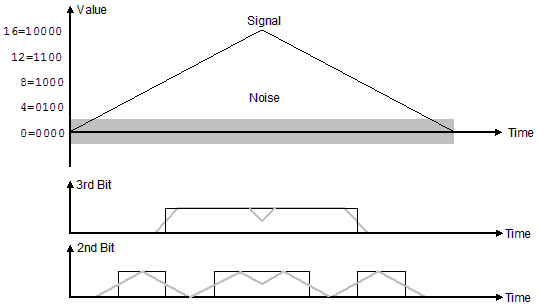
\includegraphics[height=2.5in]{Signal_and_Noise.png}
\captionof{figure}{
Effect of noise on bit values of a measured value.  The triangular wave signal and the added white noise are shown at top using the thin black line and the grey area, respectively.  The values are measured by a theoretical 4-bit Digital-to-Analog Converter in ideal condition, assuming LSB is the 0th bit.  The measured 3rd and 2nd bits without the added noise are shown using thin black lines, while the mean values of the measured 3rd and 2nd bits with the added noise are shown using thin grey lines.
This figure has been published previously \cite{Prev_Precision_Arithmetic}.
}
\label{fig: Signal_and_Noise}
\end{figure}

\begin{figure}[p]
\centering
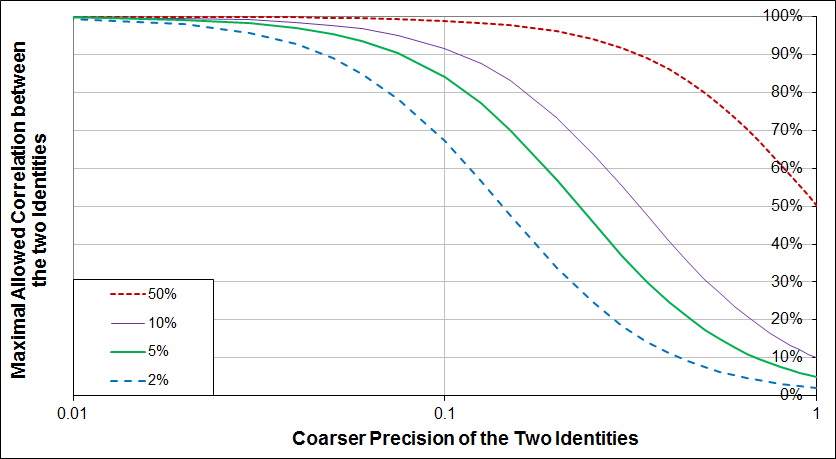
\includegraphics[height=2.5in]{Independent_Uncertainty_Assumption.png} 
\captionof{figure}{
Allowed maximal correlation between two values vs. input precisions and independence standard (as shown in legend) for the independence uncertainty assumption of variance arithmetic to be true.
This figure has been published previously \cite{Prev_Precision_Arithmetic}.
}
\label{fig: Independent_Uncertainty_Assumption}
\end{figure}

When there is a good estimation of the sources of uncertainty, the uncorrelated uncertainty assumption can be judged directly, e.g., if noise \cite{Statistical_Methods}\cite{Precisions_Physical_Measurements} is the major source of uncertainty, the uncorrelated uncertainty assumption is probably true.  
This criterion is necessary to ascertain repeated measurements of the same signal.   
Otherwise, the uncorrelated uncertainty assumption can be judged by the correlation and the respectively precision of two measurements.  

The correlated parts common to different measurements are regarded as signals, which can either be desired or unwanted.
Let $X$, $Y$, and $Z$ denote three mutually independent random variables \cite{Probability_Statistics} with variance $V(X)$, $V(Y)$ and $V(Z)$, respectively.  
Let $\alpha$ denote a constant.  
Let $Cov()$ denote the covariance function.  
Let $\gamma$ denote the correlation between $(X + Y)$ and $(\alpha X + Z)$. And let:
\begin{align}
\label{eqn: uncertainty ratio}
& \eta _{1} ^{2} \equiv \frac{V(Y)}{V(X)}; \eqspace
 \eta _{2} ^{2} \equiv \frac{V(Z)}{V(\alpha X)} =\frac{V(Z)}{\alpha ^{2} V(X)};  \\
\label{eqn: uncertainty correlation}
& \gamma =\frac{Cov(X+Y,\alpha X+Z)}{\sqrt{V(X+Y)} \sqrt{V(\alpha X+Z)}}  =\frac{\alpha /|\alpha |}{\sqrt{1+\eta _{1} ^{2} } \sqrt{1+\eta _{2} ^{2}}} \equiv \frac{\alpha /|\alpha |}{1+\eta ^{2}};
\end{align}
Formula \eqref{eqn: uncertainty correlation} gives the correlation $\gamma$ between two random variables, each of which contains a completely uncorrelated part and a completely correlated part $X$, with $\eta$ being the average ratio between these two parts.  
Formula \eqref{eqn: uncertainty correlation} can also be interpreted reversely: if two random variables are correlated by $\gamma$, each of them can be viewed hypothetically as containing a completely uncorrelated part and a completely correlated part, with $\eta$ being the average ratio between these two parts.

One special application of Formula \eqref{eqn: uncertainty correlation} is the correlation between a measured signal and its true signal, in which noise is the uncorrelated part between the two.  
Figure \ref{fig: Signal_and_Noise} shows the effect of noise on the most significant two bits of a 4-bit measured signal when $\eta=1/4$.  
Its top chart shows a triangular waveform between 0 and 16 as a black line, and a white noise between -2 and +2, using the grey area.  
The measured signal is the sum of the triangle waveform and the noise.  
The middle chart of Figure \ref{fig: Signal_and_Noise} shows the values of the 3rd digit of the true signal as a black line, and the mean values of the 3rd bit of the measurement as a grey line.  
The 3rd bit is affected by the noise during its transition between 0 and 1.  
For example, when the signal is slightly below 8, only a small positive noise can turn the 3rd digit from 0 to 1.  
The bottom chart of Figure \ref{fig: Signal_and_Noise} shows the values of the 2nd digit of the signal and the measurement as a black line and a grey line, respectively.  
Figure \ref{fig: Signal_and_Noise} clearly shows that the correlation between the measurement and the true signal is less at the 2nd digit than at the 3rd digit.  
Quantitatively, according to Formula \eqref{eqn: uncertainty correlation}:

\begin{enumerate}
\item  The overall measurement is 99.2\% correlated to the signal with $\eta=1/8$;
\item  The 3rd digit of the measurement is 97.0\% correlated to the signal with $\eta=1/4$;
\item  The 2nd digit of the measurement is 89.4\% correlated to the signal with $\eta=1/2$;
\item  The 1st digit of the measurement is 70.7\% correlated to the signal with $\eta=1$;
\item  The 0th digit of the measurement is 44.7\% correlated to the signal with $\eta=2$.
\end{enumerate}
The above conclusion agrees with the common experiences that, below the noise level of measured signals, noises rather than true signals dominate each digit.  

Similarly, while the correlated portion between two values has exactly the same value at each bit of the two values, the ratio of the uncorrelated portion to the correlated portion increases by 2-fold for each bit down from MSB of the two values. 
Quantitatively, let $P$ denote the precision of an imprecise value, and let $\eta_{P}$ denote the ratio of the uncorrelated portion to the correlated portion at level of uncertainty; then $\eta_{P}$ increases with decreased $P$ according to Formula \eqref{eqn: uncertainty level}. 
According to Formula \eqref{eqn: uncertainty correlation}, if two significant values are overall correlated with $\gamma$, at the level of uncertainty the correlation between the two values decreases to $\gamma_P$ according to Formula \eqref{eqn: uncertainty correlation}.
\begin{align}
\label{eqn: uncertainty level}
& \eta_{P} = \frac{\eta}{P}, \eqspace P < 1; \\
\label{eqn: uncertainty correlation}
& \frac{1}{\gamma_{P}} - 1 = \left(\frac{1}{\gamma} -1\right) \frac{1}{P^2}, \eqspace P < 1;
\end{align}

Figure \ref{fig: Independent_Uncertainty_Assumption} plots the relation of $\gamma$ vs. $P$ for each given $\gamma_{P}$ in Formula \eqref{eqn: uncertainty correlation}.  
When $\gamma_{P}$ is less than a predefined maximal threshold (e.g., 2\%, 5\% or 10\%), the two values can be deemed virtually uncorrelated of each other at the level of uncertainty.  
%If the two values are independent of each other at their uncertainty levels, their uncertainties are uncorrelated of each other.  
Thus for each independence standard $\gamma_{P}$, there is a maximal allowed correlation between two values below which the uncorrelated uncertainty assumption of variance arithmetic holds.  
The maximal allowed correlation is a function of the larger precision of the two values according to Formula \eqref{eqn: uncertainty correlation}.  
Figure \ref{fig: Independent_Uncertainty_Assumption} shows that for two precisely measured values, their correlation $\gamma$ is allowed to be quite high.  
Thus, the uncertainty assumption uncertainty assumption has much weaker statistical requirement than the assumption for independence arithmetic, which requires the two values to be independent of each other.

It is tempting to add noise to otherwise unqualified values to make them satisfy the uncertainties uncertainty assumption.  
As an extreme case of this approach, if two values are constructed by adding noise to the same signal, they are 50\% correlated at the uncertainty level so that they will not satisfy the uncorrelated uncertainty assumption, which defines the upper bound for $\gamma_{P}$. 
\footnote{
The 50\% curve in Figure \ref{fig: Independent_Uncertainty_Assumption} thus defines the maximal possible correlations between any two measured signals. 
This other conclusion of Formula \eqref{eqn: uncertainty correlation} makes sense because the measurable correlation between two measurements should be limited by the precision of their measurements..
}


\subsection{Result Uncertainty For Pure Rounding  \cite{Prev_Precision_Arithmetic}}

Empirically, the pure rounding error due to round-off is shown to be uniformly distributed between the half bit of the least significant bit of the siginficand \cite{Prev_Precision_Arithmetic}, whose probability density function is shown in Formula \eqref{eqn: rounding error 1/2 distribution}:
\begin{equation}
\label{eqn: rounding error 1/2 distribution}
P_{\frac{1}{2}}(x) \equiv 1, \eqspace  -1/2 \leq x \leq +1/2; 
\end{equation}



\subsection{Result Uncertainty For Addition and Subtraction  \cite{Prev_Precision_Arithmetic}}

\begin{figure}
\centering
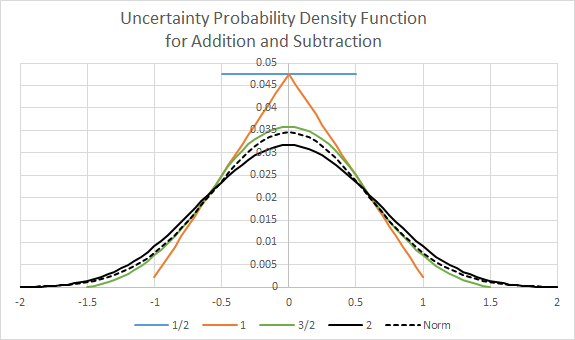
\includegraphics[height=2.5in]{Prec_Add_ErrDist.png} 
\captionof{figure}{
The probability distribution $P_{\frac{n}{2}}(x)$ of Formula \eqref{eqn:rounding error n/2 distribution}, assuming $P_{\frac{1}{2}}(x)$ is uniformly distributed between $(-1/2, +1/2)$.  
The legend shows $n$.
$P_{2}(x)$ is already close to the corresponding Gaussian distribution with the same mean and deviation, which is plotted in dash line of the same color.
This figure has been published previously \cite{Prev_Precision_Arithmetic}.
}
\label{fig: Prec_Add_Err_Dist}
\end{figure}


The uncorrelated uncertainty assumption suggests that the result bounding distribution density function of addition or subtraction is the convolution of the input density functions \cite{Probability_Statistics}.  
\begin{equation}
\label{eqn:rounding error n/2 distribution}
P_{\frac{n}{2}}(x) \equiv \int _{-\infty}^{+\infty}P_{\frac{1}{2}}(y)P_{\frac{n-1}{2}}(x-y)dy=\int _{-1/2}^{+1/2}P_{\frac{n-1}{2}}(x-y) dy,\eqspace n=2,3,4\dots;
\end{equation}
Figure \ref{fig: Prec_Add_Err_Dist} shows the probability distribution $P_{\frac{n}{2}}(x)$ of Formula \eqref{eqn:rounding error n/2 distribution}.  
$P_{2}(x)$ is already close to the corresponding Gaussian distribution with the same mean and deviation, which is plotted in dash line of the same color.

The Lyapunov form of the central limit theorem \cite{Probability_Statistics} states that if $X_i$ is a random variable with mean $\mu_i$ and variance $V_i$ for each $i$ among a series of $n$ mutually independent random variables, then with increased $n$, the sum $\sum\limits_{i}^{n} X_i$ converges in distribution to the Gaussian distribution with mean $\sum\limits_{i}^{n} \mu_i$ and variance $\sum\limits_{i}^{n} V_i$. Applying the central limit theorem to the addition and subtraction: 
\begin{itemize} 
\item $P_{n/2}(x)$ converges in distribution to a Gaussian distribution.

\item Figure \ref{fig: Prec_Add_Err_Dist} shows that such convergence to Gaussian distribution is very quick. 

\item The stable rounding error distribution is independent of any initial rounding error distribution. 
\end{itemize} 

Also due to the center-limit theorem, uncertainty in general is expected to be Gaussian distributed \cite{Statistical_Methods} \cite{Probability_Statistics}. 
The rounding error distribution is extended to describe uncertainty distribution in general.

For simplicity, define operator $\delta^2 f(x) \equiv (\delta f(x))^2$. 
Formula \eqref{eqn: addition and subtraction} give the result variance of addition and subtraction surrounding $x \pm y$.
Formula \eqref{eqn: central limit theorem} gives the probability density function for $x \pm \delta x$ in general, in which $N()$ is the density function of the  normal distribution \cite{Probability_Statistics}.
Formula \eqref{eqn: central limit theorem} can be normalized as Formula \eqref{eqn: normalized distribution}.
\begin{align}
\label{eqn: addition and subtraction}
\delta^2 (x \pm y) &= (\delta x)^2 + (\delta y)^2; \\
\label{eqn: central limit theorem}
\rho(\tilde{x}, x, \delta x) & = \frac{1}{\delta x} N(\frac{\tilde{x} - x}{\delta x}); \\
\label{eqn: normalized distribution}
\tilde{z} \equiv \frac{\tilde{x} - x}{\delta x}:\eqspace & \rho(\tilde{x}, x, \delta x) d \tilde{x} = N(\tilde{z}) d \tilde{z};
\end{align}

Formula \eqref{eqn: addition and subtraction} is different from Formula \eqref{eqn: stat +} and \eqref{eqn: stat -}, because in variance arithmetic, the correlation between $x$ and $y$ does not contribute to the result distribution as far as the uncorrelated uncertainty assumption is satisfied.
It may show that Formula \eqref{eqn: stat +} and \eqref{eqn: stat -} are wrong statistically for the result uncertainty.



\subsection{A Variance Representation}

A variance arithmetic representation uses a pair of conventional floating-point numbers to represent the value and the variance of an imprecise value.
The square root of a variance is defined as an \emph{uncertainty}.  
When the uncertainty is not specified:
\begin{itemize}
\item A conventional floating-point value has $1/\sqrt{3}$-fold of its least significant value as its uncertainty, in which the \emph{least significant value} is defined as the equivalent value of the least significant bit of the significand of the conventional floating-point value, e.g., the least significant value of $1.0$ is $2^{-52}$.
Essentially, the floating value is regarded as containing a rounding error uniformly distributed within the least significant bit of its significand.

\item An integer value within the range of $(-2^{53}, +2^{53})$ has 0 as its uncertainty.

\item An integer value outside the range of $(-2^{53}, +2^{53})$ is converted to a conventional floating-point value.
\end{itemize}


\subsection{Comparison}

\iffalse

Statistically the less relation between two imprecise values $x \pm \delta x$ and $y \pm (\delta y)^2$ is calculated by Formula \ref{eqn: x < y}:
\begin{align}
& z \equiv \frac{\tilde{y} - y}{\delta y}; \eqspace \tilde{y} = \delta y z + y; \\
& x - \Delta x < z \delta y + y < x + \Delta x; \\ & x - \Delta x - y < z \delta y < x + \Delta x - y \\
& - \Delta y < z \delta y < \Delta y; \\
p\left( x \pm (\delta x)^2 < y \pm (\delta y)^2 \right) & = 
  \int_{y - \Delta y}^{y + \Delta y} \rho(\tilde{y}, y, \delta y) 
    \int_{x - \Delta x}^{\tilde{y}} \rho(\tilde{x}, x, \delta x) d \tilde{x} \;d \tilde{y}; \\
& = \int_{y - \Delta y}^{y + \Delta y} \rho(\tilde{y}, y, \delta y) 
  \int_{-\frac{\Delta x}{\delta x}}^{\frac{\tilde{y} - x}{\delta x}} N(z) d z \;d \tilde{y}; \\
& = \int_{y - \Delta y}^{y + \Delta y} \rho(\tilde{y}, y, \delta y) 
      \frac{1}{2}(\frac{\tilde{y} - x}{\sqrt{2} \delta x}) - \zeta(\frac{-\Delta x}{\sqrt{2} \delta x})) \;d \tilde{y}; \\
& = \int_{\frac{\max(-\Delta y, x - \Delta x - y)}{\delta y}}^{\frac{\min(+\Delta y, x + \Delta x - y)}{\delta y}} 
      \frac{1}{2} \left(\zeta(\frac{z \delta y + y - x}{\sqrt{2} \delta x}) - \zeta(-\frac{\Delta x}{\sqrt{2} \delta x})\right) N(z) d z; \\
p\left( x \pm (\delta x)^2 > y \pm (\delta y)^2 \right) & =     
   \int_{\frac{\max(-\Delta y, x - \Delta x - y)}{\delta y}}^{\frac{\min(+\Delta y, x + \Delta x - y)}{\delta y}} 
      \frac{1}{2} \left(\zeta(+\frac{\Delta x}{\sqrt{2} \delta x}) - \zeta(\frac{z \delta y + y - x}{\sqrt{2} \delta x})\right) N(z) d z;
\end{align}
Formula \eqref{eqn: x < y} seems correct because it predicts $p(x \le y) = p(y \ge x)$:
\begin{align}
& \frac{d}{d \tilde{y}} \int_{-\infty}^{\tilde{y}} \rho(\tilde{x}, x, \delta x) d \tilde{x} = \rho(\tilde{y}, x, \delta x); \\
p(x< y) & = \int_{-\infty}^{+\infty} \rho(\tilde{y}, y, \delta y) \rho(\tilde{y}, x, \delta x) d \tilde{x} d \tilde{y} \\
& = \int_{-\infty}^{+\infty} \rho(\tilde{y}, y, \delta y) \;d \rho(\tilde{y}, x, \delta x) \\
& = 0 - \int_{-\infty}^{+\infty} \rho(\tilde{y}, x, \delta x) \;d \rho(\tilde{y}, y, \delta y) \\
& = \int_{-\infty}^{+\infty} \rho(\tilde{y}, x, \delta x) 
\int_{\tilde{y}}^{+\infty} \rho(\tilde{x}, y, \delta y) 
d \tilde{x} \;d \tilde{y} \\
& = \int_{-\infty}^{+\infty} \rho(\tilde{x}, x, \delta x) 
\int_{\tilde{x}}^{+\infty} \rho(\tilde{y}, y, \delta y) 
d \tilde{y} \;d \tilde{x}
\end{align}

Two imprecise values can be compared directly for less or greater relation when their ranges $(x - \Delta x, x + \Delta x)$ and $(y - \Delta y, y + \Delta y)$ do not overlap. 
Otherwise, statistically, Formula \eqref{eqn: x < y} and \eqref{eqn: x > y} gives the probability for less or greater relation between $x \pm (\delta x)^2 \le y \pm (\delta y)^2$, in which $\min()$ and $\max()$ are minimal and maximal functions, respectively.
Formula \eqref{eqn: no =} shows that two imprecise variable can not be equal statistically.
Let $x = y$, $\delta x = \delta y$ and $\Delta x = \Delta y$, Formula \eqref{eqn: x < y} and \eqref{eqn: x > y} shows that two conceptually equal imprecise values has $1/2$ chance to be one less than the other, and $1/2$ chance to be one more than the other.
Thus,
\begin{align}
\label{eqn: x < y}
& p\left( x \pm (\delta x)^2 < y \pm (\delta y)^2 \right) = 
  \int_{\frac{\max(-\Delta y, x - \Delta x - y)}{\delta y}}^{\frac{\min(+\Delta y, x + \Delta x - y)}{\delta y}} 
      \frac{1}{2} \left(\zeta(\frac{z \delta y + y - x}{\sqrt{2} \delta x}) - \zeta(-\frac{\Delta x}{\sqrt{2} \delta x})\right) N(z) d z; \\
\label{eqn: x > y}
& p\left( x \pm (\delta x)^2 > y \pm (\delta y)^2 \right) =     
  \int_{\frac{\max(-\Delta y, x - \Delta x - y)}{\delta y}}^{\frac{\min(+\Delta y, x + \Delta x - y)}{\delta y}} 
      \frac{1}{2} \left(\zeta(+\frac{\Delta x}{\sqrt{2} \delta x}) - \zeta(\frac{z \delta y + y - x}{\sqrt{2} \delta x})\right) N(z) d z; \\
\label{eqn: no =}
& p\left( x \pm (\delta x)^2 < y \pm (\delta y)^2 \right) + p\left( x \pm (\delta x)^2 > y \pm (\delta y)^2 \right) = 1;
\end{align}

\fi

Two imprecise values can be compared statistically using their difference.

When the value difference is zero, the two imprecise values are equal.  
Such definition of equality deviates from statistics.
In statistics, such two imprecise value has $50\%$ possibility to be less than or greater to each other but no chance to be equal to each other.

Otherwise, the standard z-method \cite{Probability_Statistics} is used to judge whether they are equal to each other, or less or more than each other.
For example, the difference between $1.002 \pm 0.001$ and $1.000 \pm 0.002$ is $0.002 \pm 0.00224$, so that the z-value for the difference is $z = 0.002 / 0.00224$, and the probability for them to be not equal is $\xi(|z|) - \xi(-|z|) = 62.8\%$, in which $\xi(z)$ is the cumulative density function for normal distribution \cite{Probability_Statistics}.
If the threshold probability of not equality is $50\%$, $1.000 \pm 0.002 < 1.002 \pm 0.001$.
Instead of using the threshold probability, the bounding range for z can be used, such as $|z| \leq 0.67448975$ for the equivalent threshold probability of $50\%$.






\subsection{Multiplication}

\iffalse
\begin{align*}
0 \leq |x| - \Delta x, 0 \leq |y| - \Delta y: &\eqspace 
	(|x||y| - |x| \Delta y - |y| \Delta x + \Delta x \Delta y, |x||y| + |x| \Delta y + |y| \Delta x + \Delta x \Delta y) \\
&\eqspace \Delta xy = |x| \Delta y + |y| \Delta x; \\
|x| - \Delta x \leq 0 \leq |y| - \Delta y: &\eqspace 
    (|x||y| + |x| \Delta y - |y| \Delta x - \Delta x \Delta y, |x||y| + |x| \Delta y + |y| \Delta x + \Delta x \Delta y) \\
&\eqspace \Delta xy = |y| \Delta x + \Delta x \Delta y; \\
|x| - \Delta x \leq 0, \; |y| - \Delta y \leq 0: &\eqspace
	(|x||y| + |x| \Delta y - |y| \Delta x - \Delta x \Delta y, |x||y| + |x| \Delta y + |y| \Delta x + \Delta x \Delta y) \\
&\eqspace \Delta xy = |y| \Delta x + \Delta x \Delta y;
\end{align*}
But the range needs to be centered at $|x||y|$.
\fi

To obey the precision scaling principle, the result of multiplying $x \pm \delta x$ by a precise value $y$ is $ y^2 \delta^2 x$.
The result of multiplying $0 \pm \delta x$ by $0 \pm \delta y$ is a normal production distribution \cite{Probability_Statistics}, which is centered at 0 with variance $(\delta x)^2 (\delta y)^2$.
The general multiplication can be decomposed as Formula \eqref{eqn: multiplication decomposed}, which leads to Formula \eqref{eqn: multiplication}  \cite{Prev_Precision_Arithmetic} and \eqref{eqn: multiplication precision}  \cite{Prev_Precision_Arithmetic} for the result variance and precision surrounding the result $xy$, respectively.
\begin{align}
\label{eqn: multiplication decomposed}
& (x \pm \delta x) \times (y \pm \delta y) = (x + (0 \pm \delta x)) \times (y + (0 \pm \delta y)); \\
\label{eqn: multiplication}
\delta^2 (x y) &= x^2 (\delta^2 y) + y^2 (\delta^2 x) + (\delta^2 x)(\delta^2 y); \\
\label{eqn: multiplication precision}
xy \neq 0: P(x y)^2 &= P(x)^2 + P(y)^2 + P(x)^2 P(y)^2;
\end{align}

Formula \eqref{eqn: multiplication} is identical to Formula \eqref{eqn: stat *} for statistical propagation of uncertainty except their cross term, representing difference in their statistical requirements, respectively.  
Formula \eqref{eqn: multiplication} is simpler and more elegant than Formula \eqref{eqn: interval *} for the interval arithmetic multiplication.  
The result of Formula \eqref{eqn: float num calc} calculated by variance arithmetic is $2 \pm 2\sqrt{5}$.
It is $2 \pm 9$ for interval arithmetic \cite{Worst_Case_Error_Bounds}.




\subsection{Uncertainty Distribution}

\iffalse

To solve for mode:
\begin{align*}
& \rho(\tilde{y}, y, \delta y) = \frac{d \tilde{z}}{d \tilde{y}} N(\tilde{z});
\eqspace \tilde{z} = \frac{f^{-1}(\tilde{y}) - x}{\delta x}; \\
& 0 = \frac{d \rho(\tilde{y}, y, \delta y)}{d \tilde{y}} = \frac{d^2 \tilde{z}}{d \tilde{y}^2} N(\tilde{z}) - \frac{d \tilde{z}}{d \tilde{y}} N(\tilde{z}) \tilde{z}; \\
& \frac{d^2 \tilde{z}}{d \tilde{y}^2} = \frac{d \tilde{z}}{d \tilde{y}} \tilde{z}; \eqspace \tilde{z} = \frac{f^{-1}(\tilde{y}) - x}{\delta x};
\end{align*}

The exponential function:
\begin{align*}
f(x) = e^x:& \eqspace 
\tilde{z} = \frac{\log(\tilde{y}) - x}{\delta x}, \eqspace 
\frac{d \tilde{z}}{d \tilde{y}} = \frac{1}{\tilde{y} \delta x} = \frac{1}{\frac{d}{d \tilde{z}} e^{x + \tilde{z} \delta x}}; \eqspace \\
\frac{d \tilde{z}}{d \tilde{y}} N(\tilde{z})
&= e^{-\log(\tilde{y})} \frac{1}{\sqrt{2\pi} \delta x} e^{-\frac{(\log(\tilde{y}) - x)^2}{2 \delta^2 x}}
 = \frac{1}{\sqrt{2\pi} \delta x} e^{-\frac{(\log(\tilde{y}) - x)^2 + 2 \log(\tilde{y}) \delta^2 x }{2 \delta^2 x}} \\
& = \frac{1}{\sqrt{2\pi} \delta x} e^{-\frac{(\log(\tilde{y}) - (x - \delta^2 x))^2 + 2 x \delta^2 x - (\delta^2 x)^2 }{2 \delta^2 x}}
 = N(\frac{\log(\tilde{y}) - (x - \delta^2 x)}{\delta x}) e^{-x + \frac{\delta^2 x}{2}}; \\
& 0 = \tilde{z} e^{x + \tilde{z} \delta x} + (\delta x) e^{x + \tilde{z} \delta x}; \eqspace
 \tilde{z} = -(\delta x) = \frac{1}{\delta x}(x - (\delta x)^2 - x);
\end{align*}

The log function $f(x) = \ln(x)$:
\begin{align*}
& \tilde{z} = \frac{e^{\tilde{y}} - x}{\delta x}; \eqspace 
\frac{d \tilde{z}}{d \tilde{y}} = \frac{1}{\delta x} e^{\tilde{y}} = \frac{1}{\delta x} (x + \tilde{z} \delta x)
 = \frac{1}{\frac{d}{d \tilde{z}} \ln(x + \tilde{z} \delta x)}; \\
& \frac{1}{\delta x} e^{\tilde{y}} = (\frac{1}{\delta x} e^{\tilde{y}})^2 \frac{e^{\tilde{y}} - x}{\delta x}; \eqspace 
(e^{\tilde{y}})^2 - x e^{\tilde{y}} - \delta^2 x = 0; \\
e^{\tilde{y}_m} &= \frac{x + \sqrt{x^2 + 4 \delta^2 x}}{2}; \\
& \eqspace 0 = \frac{\tilde{z}}{x + \tilde{z} \delta x} - (\delta x) \frac{1}{(x + \tilde{z} \delta x)^2}; \eqspace
0 = (\delta x) \tilde{z}^2 + x \tilde{z} - (\delta x); \\
& \tilde{z} = \frac{1}{\delta x}(\frac{x + \sqrt{x^2 + 4 (\delta x)^2}}{2} - x);
\end{align*}

The power mode $f(x) = x^{\frac{1}{p}}$:
\begin{align*}
& \tilde{z} = \frac{\tilde{y}^p - x}{\delta x}; \eqspace 
\frac{d \tilde{z}}{d \tilde{y}} = \frac{1}{\delta x} p \tilde{y}^{p-1}; \\
& \frac{1}{\delta x} p (p - 1) \tilde{y}^{p-2} = (\frac{1}{\delta x} p \tilde{y}^{p-1})^2 \frac{\tilde{y}^p - x}{\delta x}; \\
& \tilde{y}^{2p} - x \tilde{y}^{p} - \frac{p - 1}{p} \delta^2 x = 0; \\
\tilde{y}_m^p &= \frac{1}{2} (x + \sqrt{x^2 + 4 \frac{p - 1}{p} \delta^2 x}); \\
& 0 = c (x + \tilde{z} \delta x)^{c-1} \tilde{z} + c (c-1) \delta x (x + \tilde{z} \delta x)^{c-2}; \eqspace
0 = (\delta x) \tilde{z}^2 + x \tilde{z} + (c - 1) (\delta x); \\
& \tilde{z}_m = \frac{1}{\delta x}(\frac{x + \sqrt{x^2 - 4(c-1)(\delta x)^2}}{2} - x); \eqspace 
f^{-1}(\tilde{y}_m) = \frac{x + \sqrt{x^2 - 4(c-1)(\delta x)^2}}{2}; \\
p = 2:& \eqspace \frac{d \tilde{z}}{d \tilde{y}} = \frac{1}{\delta x} 2 \tilde{y}; \eqspace 
  \tilde{y}_m^{\frac{1}{2}} = \frac{1}{2} \left( x + \sqrt{x^2 + 2 \delta^2 x} \right); \\
p = 3:& \eqspace \frac{d \tilde{z}}{d \tilde{y}} = \frac{1}{\delta x} 3 \tilde{y}^2; \eqspace  
  \tilde{y}_m^{\frac{1}{3}} = \frac{1}{2} \left( x \pm \sqrt{x^2 + \frac{8}{3} \delta^2 x} \right); \\
p = 1/2:& \eqspace \frac{d \tilde{z}}{d \tilde{y}} = \frac{1}{\delta x} \frac{1}{2} \tilde{y}^{-\frac{1}{2}}; \eqspace 
  \tilde{y}_m^2 = \frac{1}{2} \left( x + \sqrt{x^2 - 4 \delta^2 x} \right); \\
p = 1/3:& \eqspace \frac{d \tilde{z}}{d \tilde{y}} = \frac{1}{\delta x} \frac{1}{3} \tilde{y}^{-\frac{2}{3}}; \eqspace
  \tilde{y}_m^2 = \frac{1}{2} \left( x \pm \sqrt{x^2 - 8 \delta^2 x} \right); \\
p = -1:& \eqspace \frac{d \tilde{z}}{d \tilde{y}} = - \frac{1}{\delta x} \tilde{y}^{-2}; \eqspace 
  \tilde{y}_m^{-1} = \frac{1}{2} \left( x + \sqrt{x^2 + 8 \delta^2 x} \right); 
\end{align*}


The distribution difference:
\begin{align*}
&\nu = \frac{x - f^{-1}(\tilde{y}_m)}{\delta x}: \eqspace 
 N(\frac{f^{-1}(\tilde{y}) - f^{-1}(\tilde{y}_m)}{\delta x} )
 = N(\tilde{z} + \nu) = N(\tilde{z}) e^{-\tilde{z} \nu} e^{-\frac{1}{2} \nu^2}; \\
\eta &\equiv \int |\varrho(\tilde{y}, y, \delta y) - \rho(\tilde{y}, y, \delta y)| d \tilde{y}
 =  \int |\rho(f^{-1}(\tilde{y}), f^{-1}(\tilde{y_m}), \delta x) - \rho(f^{-1}(\tilde{y}), x, \delta x)| d f^{-1}(\tilde{y}) \\
&= \int |N(\tilde{z} + \nu) - N(\tilde{z})| d \tilde{z} 
 = \int |e^{-\frac{1}{2} \nu^2} e^{-\tilde{z} \nu} - 1| N(\tilde{z}) d \tilde{z}; \\
&= | \int |\sum_{m=0}^{\infty} \frac{(-\nu^2)^m}{2^m m!} \sum_{n=0}^{\infty} \frac{(-\nu)^n}{n!} \tilde{z}^n - 1| 
   N(\tilde{z}) d \tilde{z} | \\
&= | \int \left(\sum_{m=1}^{\infty} \frac{(-\nu^2)^m}{2^m m!} \sum_{n=1}^{\infty} \frac{(-\nu)^n}{n!} \tilde{z}^n
  - \frac{1}{2} \nu^2 - \nu \tilde{z} \right) N(\tilde{z}) d \tilde{z} | \\
&= \frac{1}{2} \nu^2 - \sum_{m=1}^{\infty} \frac{(-\nu^2)^m}{2^m m!} \sum_{n=1}^{\infty} \frac{\nu^{2n}}{2^n n!}
 = \frac{1}{2} \nu^2 - \sum_{m=2}^{\infty} \sum_{n=1}^{m-1} \frac{(-1)^m}{2^m (m - n)! n!} \nu^{2m} \\
&\simeq \frac{1}{2} \nu^2 - \frac{1}{4} \nu^4 + \frac{1}{8} \nu^6 - \frac{7}{192} \nu^8;
\end{align*}
When $f(x)=x^c$:
\begin{align*}
\nu &= \frac{x - \frac{1}{2} (x + \sqrt{x^2 + (1 - c) 4 \delta^2 x})}{\delta x} = \frac{1 - \sqrt{1 + (1 - c) 4 P(x)^2}}{2 P(x)} \\
&= - \sum_{m=1} \frac{(1 - c)^m (2P(x))^{2m - 1}}{m!} \prod_{n=1}^{m} \frac{\frac{3}{2} -n}{n} \\
&\simeq -(1 - c) P(x) + \frac{1}{4} (1 - c)^2 P(x)^3 - \frac{1}{4} (1 - c)^3 P(x)^5; \\
\eta &= \frac{1}{2} (1-c)^2 P(x)^2 - \frac{1}{4} (1-c)^3 (2-c) P(x)^4 + 1/8 (1-c)^4 (c^2-4c+7) P(x)^6
\end{align*}

\fi

\begin{figure}[p]
\centering
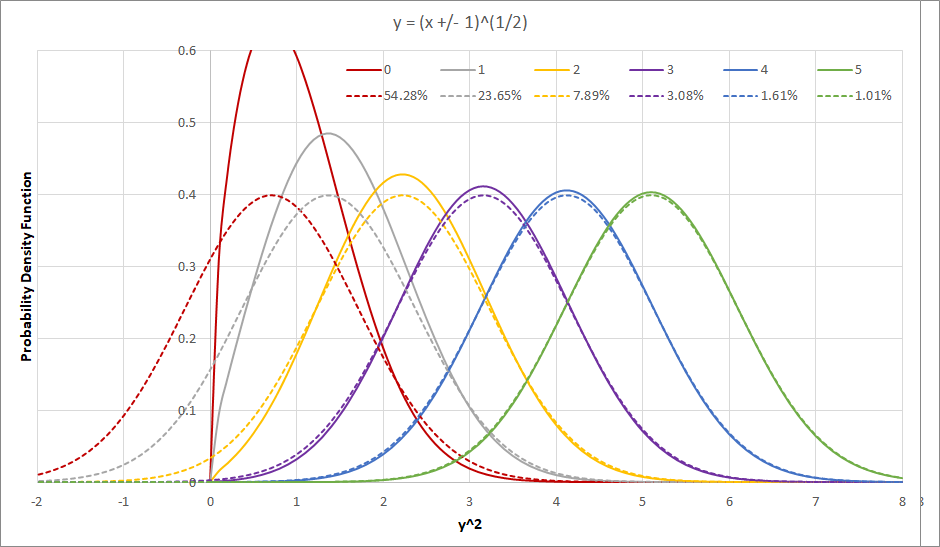
\includegraphics[height=2.5in]{Square_Root_Distribution.png} 
\captionof{figure}{
The probability density function for $\tilde{y} = \sqrt{x \pm 1}$, for different $x$ as shown in the legend. 
The $x$-axis is scaled as $\tilde{y}^2$.
Each probability density function $\rho(\tilde{x})$ in solid line is compared with a Gaussian distribution $\varrho(\tilde{x})$ of the same mode and the same deviation in the dash line of the same color.
The legend for the Gaussian distribution shows the value of Gaussian difference in percentage.
}
\label{fig: Square_Root_Distribution}
\end{figure}

\begin{figure}[p]
\centering
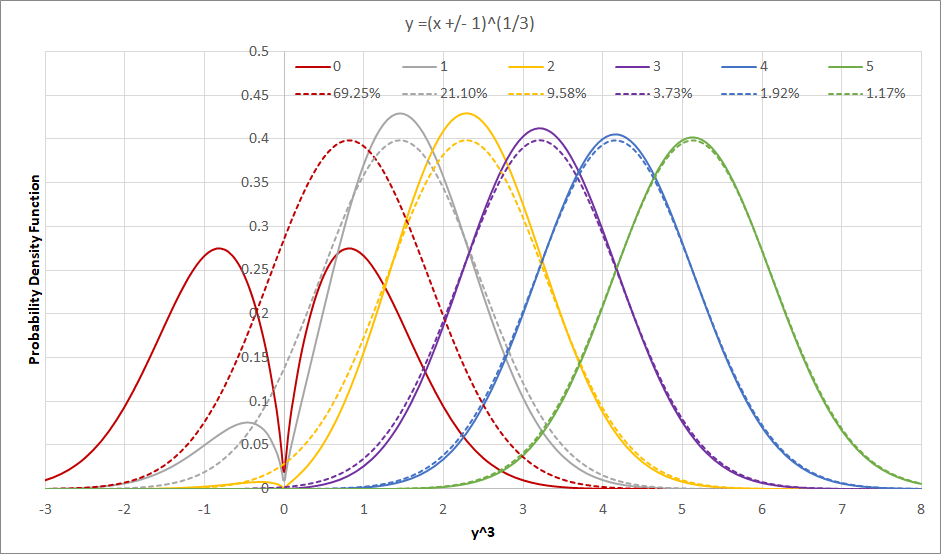
\includegraphics[height=2.5in]{Cubic_Root_Distribution.png} 
\captionof{figure}{
The probability density function for $\sqrt[3]{x \pm 1}$, for different $x$ as shown in the legend. 
The $y$-axis is scaled as $\tilde{y}^3$.
Each probability density function $\rho(\tilde{x})$ in solid line is compared with a Gaussian distribution $\varrho(\tilde{x})$ of the same mode and the same deviation in the dash line of the same color.
The legend for the Gaussian distribution shows the value of Gaussian difference in percentage.
}
\label{fig: Cubic_Root_Distribution}
\end{figure}

\begin{figure}[p]
\centering
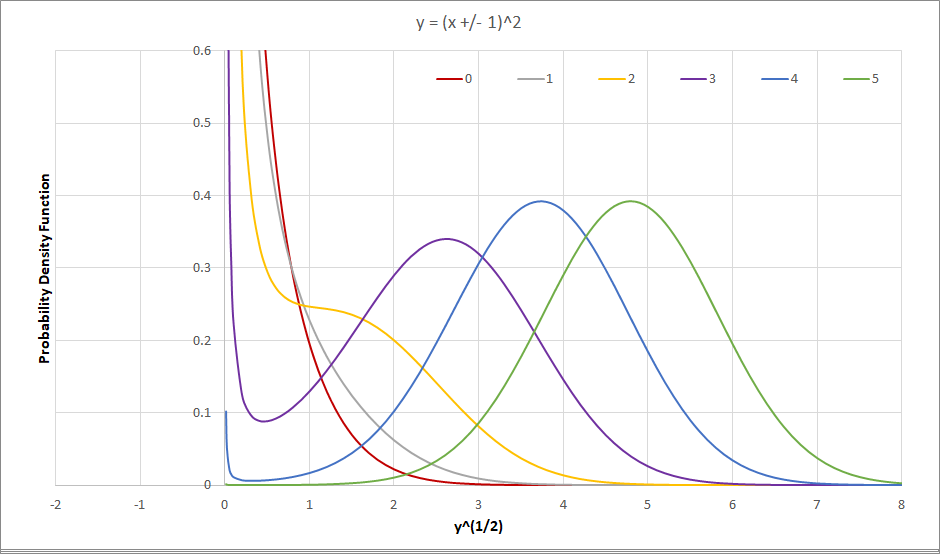
\includegraphics[height=2.5in]{Square_Distribution.png} 
\captionof{figure}{
The probability density function for $(x \pm 1)^2$, for different $x$ as shown in the legend. 
The $y$-axis is scaled as $\sqrt{\tilde{y}}$.
Some probability density function $\rho(\tilde{x})$ in solid line is compared with a Gaussian distribution $\varrho(\tilde{x})$ of the same mode and the same deviation in the dash line of the same color.
The legend for the Gaussian distribution shows the value of Gaussian difference in percentage.
}
\label{fig: Square_Distribution}
\end{figure}

\begin{figure}[p]
\centering
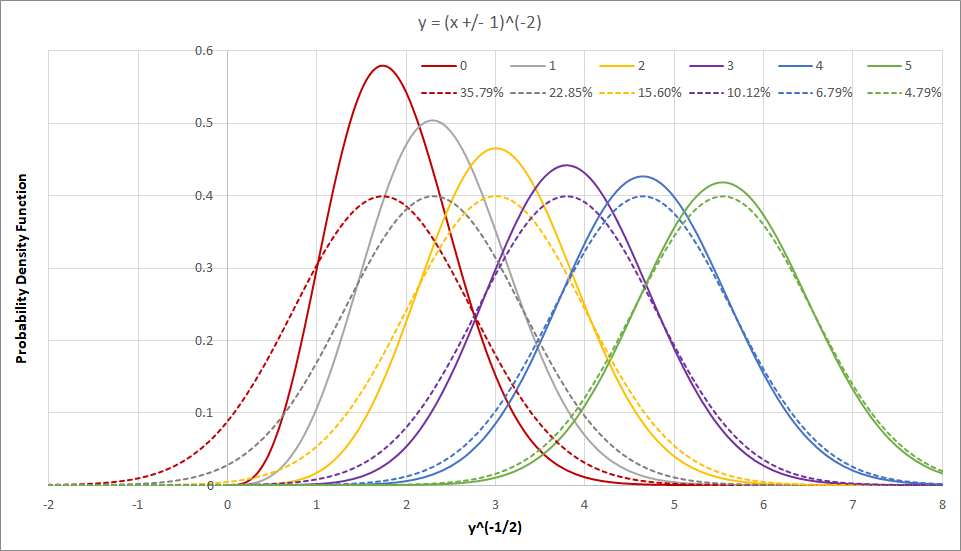
\includegraphics[height=2.5in]{Inverse_Square_Distribution.png} 
\captionof{figure}{
The probability density function for $1/(x \pm 1)^2$, for different $x$ as shown in the legend. 
The $y$-axis is scaled as $1/\sqrt{\tilde{y}}$.
The probability density function $\rho(\tilde{x})$ in solid line is compared with a Gaussian distribution $\varrho(\tilde{x})$ of the same mode and the same deviation in the dash line of the same color.
The legend for the Gaussian distribution shows the value of Gaussian difference in percentage.
}
\label{fig: Inverse_Square_Distribution}
\end{figure}


Let $\tilde{y} = f(\tilde{x})$ be a strictly monotonic function, so that $\tilde{x} = f^{-1}(\tilde{y})$ exist.
Formula \eqref{eqn: function distribution} is the uncertainty distribution density function \cite{Statistical_Methods}.
In Formula \eqref{eqn: function distribution} \cite{Statistical_Methods}, the same distribution can be expressed in either $\tilde{x}$ or $\tilde{y}$ or $\tilde{z}$ , which are different representations of the same underlying random variable.
Using Formula \eqref{eqn: function distribution}, Formula \eqref{eqn: exp distribution}, \eqref{eqn: log distribution}, and \eqref{eqn: power distribution} give the $\rho(\tilde{y}, y, \delta y)$ for $e^x$, $\ln(x)$, and $x^c$, respectively.
\begin{align}
\label{eqn: function distribution}
N(\tilde{z}) d \tilde{z} = \rho(\tilde{x}, x, \delta x) d\tilde{x} &= \rho(f^{-1}(\tilde{y}), x, \delta x) \frac{d\tilde{x}}{d\tilde{y}} d\tilde{y} 
= \rho(\tilde{y}, y, \delta y) d\tilde{y}; \\
\label{eqn: exp distribution}
y = e^x: &\; \rho(\tilde{y}, y, \delta y) = \frac{1}{\tilde{y}} \frac{1}{\delta x} N(\frac{\log(\tilde{y}) - x}{\delta x}); \\
\label{eqn: log distribution}
y = \ln(x): &\; \rho(\tilde{y}, y, \delta y) = e^{\tilde{y}} \frac{1}{\delta x} N(\frac{e^{\tilde{y}} - x}{\delta x}); \\
\label{eqn: power distribution}
y = x^c: &\; \rho(\tilde{y}, y, \delta y) = c \tilde{y}^{\frac{1}{c}-1} \frac{1}{\delta x} N(\frac{\tilde{y}^\frac{1}{c} - x}{\delta x}); 
\end{align}
Using Formula \eqref{eqn: function distribution}, Formula \eqref{eqn: distribution mode} gives the equation for the mode of the result distribution, whose solutions $f^{-1}(\tilde{y}_m)$ for $e^x$, $\ln(x)$, and $x^c$ are Formula \eqref{eqn: exp mode}, \eqref{eqn: log mode}, and \eqref{eqn: power mode} respectively.
\begin{align}
\label{eqn: distribution mode}
\eqspace \tilde{z} = \frac{f^{-1}(\tilde{y}) - x}{\delta x}: &\eqspace \frac{d^2 \tilde{z}}{d \tilde{y}^2} = \frac{d \tilde{z}}{d \tilde{y}} \tilde{z}; \\
\label{eqn: exp mode}
\tilde{y} = e^{\tilde{x}}: &\eqspace \ln(\tilde{y}_m) = x - (\delta x)^2; \\
\label{eqn: log mode}
\tilde{y} = \ln(\tilde{x}): &\eqspace e^{\tilde{y}_m} = \frac{x + \sqrt{x^2 + 4 (\delta x)^2}}{2}; \\
\label{eqn: power mode}
\tilde{y} = \tilde{x}^c: &\eqspace (\tilde{y}_m)^{1/c} = \frac{x + \sqrt{x^2 - 4(c-1)(\delta x)^2}}{2};
\end{align}

The \emph{Gaussian difference} of $\rho(f^{-1}(\tilde{y}), x, \delta x)$ is calculated as $\int_{-\infty}^{+\infty} |\rho(f^{-1}(\tilde{y}), x, \delta x) - \varrho(\tilde{y})| d \tilde{y}$ in which $\varrho(\tilde{y})$ is the Gaussian distribution of the same mode and the same deviation $\delta x$.
A Gaussian difference of 0 means a perfect Gaussian.

Viewed in the $f^{-1}(\tilde{y})$ coordinate, $\rho(\tilde{y}, y, \delta y)$ is Gaussian modulated by $\frac{d\tilde{x}}{d\tilde{y}} = 1/f^{(1)}_x$.
A \emph{zero} of the uncertainty distribution happens when $f^{(1)}_x=\infty \rightarrow \rho(\tilde{y}, y, \delta y) = 0$, while a \emph{pole} happens when $f^{(1)}_x=0 \rightarrow \rho(\tilde{y}, y, \delta y) = \infty$.
Zeros and poles have different impacts on the properties of of the uncertainty distributions.

If $y=f(x)$ is a linear transform of $x$, $f^{(1)}_x$ is a constant, and $\rho(\tilde{y}, y, \delta y)$ is known to be Gaussian \cite{Probability_Statistics}.
From another prospective, a linear transformation generates neither zero nor pole according Formula \eqref{eqn: function distribution}.

Figure \ref{fig: Square_Root_Distribution} shows the probability density function for $\sqrt{x \pm 1}$ according to Formula \eqref{eqn: power distribution}, which has a zero at $x=0$.
Each probability density function $\rho(\tilde{x})$ in solid line is compared with a normal distribution $\varrho(\tilde{x})$ of the same mode in dash line of the same color.

Figure \ref{fig: Cubic_Root_Distribution} shows the probability density function for $\sqrt[3]{x \pm 1}$ according to Formula \eqref{eqn: power distribution}, which also has a zero at $x=0$.
Compared with $\sqrt{x \pm 1}$, $\sqrt[3]{x \pm 1}$ distributes on $\tilde{y} < 0$ also, so that the uncertainty distributions for $\sqrt[3]{0 \pm 1}$ has two equal peaks instead of one larger peak on the positive side only for $\sqrt{x \pm 1}$.

Figure \ref{fig: Square_Distribution} shows the probability density function for $(x \pm 1)^2$ according to Formula \eqref{eqn: power distribution}, which has a pole at $x=0$.
The uncertainty distributions for $(0 \pm 1)^2$ and $(1 \pm 1)^2$ deviate significantly from Gaussian, while the uncertainty distributions for $(4 \pm 1)^2$ and $(5 \pm 1)^2$ look Gaussian but each still with an infinitive but narrower peak at $\tilde{y} = 0$.
According to Formula \eqref{eqn: power mode}, $(0 \pm 1)^2$ and $(1 \pm 1)^2$ has no mode.
$(0 \pm 1)^2$ is actually the $\chi^2$ distribution \cite{Statistical_Methods}.

Figure \ref{fig: Inverse_Square_Distribution} shows the probability density function for $1/(x \pm 1)^2$ according to Formula \eqref{eqn: power distribution}, which has a zero at $x=0$.
Figure \ref{fig: Inverse_Square_Distribution} looks more like Figure \ref{fig: Square_Root_Distribution} than Figure \ref{fig: Square_Distribution}, showing that pole or zero determines the properties of uncertainty distributions.

In all the figures, the probability density function in the $\tilde{z}$ representation becomes more Gaussian-like when the mode of the distributions is further away from either zero or pole.
Such observation leads to the following Taylor method to calculate the result variances when the distribution is nearly Gaussian in the $\tilde{z}$ representation.
 



\subsection{Analytic Functions}

\iffalse

\begin{align*}
& \tilde{y} = f(x + \tilde{z} \delta x) = \sum_{n=0}^{\infty} \frac{f^{(n)}_x}{n!} \tilde{z}^n (\delta x)^n; \\
\overline{f(x)} &\equiv \int \tilde{y} \rho(\tilde{y}, y, \delta y) d \tilde{y}
 = \int \sum_{n=0}^{\infty} \frac{f^{(n)}_x}{n!} \tilde{z}^n (\delta x)^n N(\tilde{z}) d \tilde{z}
 = \sum_{n=0}^{\infty} \frac{f^{(n)}_x}{n!} (\delta x)^{n} \int \tilde{z}^n N(\tilde{z}) d \tilde{z} \\
&= \sum_{n=0}^{\infty} \frac{f^{(n)}_x}{n!} (\delta x)^{n} \zeta(n)
 = \sum_{n=0}^{\infty} \frac{f^{(2n)}_x}{(2n)!} (\delta x)^{2n} \zeta(2n); \\
\delta^2 f(x) &\equiv \int \tilde{y}^2 \rho(\tilde{y}, y, \delta y) d \tilde{y} - \overline{f(x)}^2
 = \int (\sum_{n=0}^{\infty} \frac{f^{(n)}_x}{n!} \tilde{z}^n (\delta x)^n)^2 N(\tilde{z}) d \tilde{z} - \overline{f(x)}^2 \\
&= \sum_{n=0}^{\infty} \sum_{j=0}^{2n} \frac{f^{(j)}_x}{j!} \frac{f^{(2n-j)}_x}{(2n-j)!} (\delta x)^{2n} \zeta(2n)
 - \sum_{n=0}^{\infty} \sum_{j=0}^{n} \frac{f^{(2j)}_x}{(2j)!} \frac{f^{(2n-2j)}_x}{(2n-2j)!} (\delta x)^{2n} \zeta(2j) \zeta(2n - 2j) \\
&= \sum_{n=1}^{\infty} (\delta x)^{2n} ( \zeta(2n) \sum_{j=1}^{2n-1} \frac{f^{(j)}_x}{j!} \frac{f^{(2n-j)}_x}{(2n-j)!}
  - \sum_{j=1}^{n-1} \frac{f^{(2j)}_x \zeta(2j)}{(2j)!} \frac{f^{(2n-2j)}_x \zeta(2n - 2j)}{(2n-2j)!} \\
&\eqspace + 2 \zeta(2n) f(x) \frac{f^{(2n)}_x}{(2n)!} - 2 f(x) \frac{f^{(2n)}_x \zeta(2n)}{(2n)!}) \\
&= \sum_{n=1}^{\infty} (\delta x)^{2n} \left( \zeta(2n) \sum_{j=1}^{2n-1} \frac{f^{(j)}_x}{j!} \frac{f^{(2n-j)}_x}{(2n-j)!}
  - \sum_{j=1}^{n-1} \frac{f^{(2j)}_x \zeta(2j)}{(2j)!} \frac{f^{(2n-2j)}_x \zeta(2n - 2j)}{(2n-2j)!} \right) \\
&= (\delta x)^2 (f^{(1)}_x)^2 + (\delta x)^4 \left(f^{(1)}_x f^{(3)}_x + \frac{1}{2} (f^{(2)}_x)^2 \right) \\
&\eqspace + (\delta x)^6 \left(\frac{1}{4} f^{(1)}_x f^{(5)}_x + \frac{1}{2} f^{(2)}_x f^{(4)}_x + \frac{5}{12} (f^{(3)}_x)^2 \right) + o((\delta x)^8); \\
\delta^2 f(x) &= \sum_{n=1}^{\infty} (\delta x)^{2n} \zeta(2n) \sum_{j=0}^{2n} \frac{f^{(j)}_x}{j!} \frac{f^{(2n-j)}_x}{(2n-j)!} - \overline{f(x)}^2 \\
  &= \sum_{n=1}^{\infty} (\delta x)^{2n} \frac{\zeta(2n)}{(2n)!} (f(x)^2)^{(2n)}_x - \overline{f(x)}^2; \\
  &= (\delta x)^2 (f(x) f^{(2)}_x + (f^{(1)}_x)^2 - f(x) f^{(2)}_x) \\
  &\eqspace + (\delta x)^4 (\frac{1}{4} f(x) f^{(4)}_x + f^{(1)}_x f^{(3)}_x + \frac{3}{4} (f^{(2)}_x)^2 - \frac{1}{4} f(x) f^{(4)}_x - \frac{1}{4} (f^{(2)}_x)^2)    \\
  & = (\delta x)^2 (f^{(1)}_x)^2 + (\delta x)^4 (f^{(1)}_x f^{(3)}_x + \frac{1}{2} (f^{(2)}_x)^2) + o((\delta x)^6);  \\
\overline{f(x)} &= f(x) + (\delta x)^2 \frac{1}{2} f^{(2)}_x + (\delta x)^4 \frac{1}{8} f^{(4)}_x + o((\delta x)^6); \\
f(x + \tilde{x})^2 &= f(x)^2 + \frac{\tilde{x}}{1!} (2 f(x) f^{(1)}_x) + \frac{\tilde{x}^2}{2!} (2 f(x) f^{(2)}_x + 2 (f^{(1)}_x)^2) \\
&\eqspace + \frac{\tilde{x}^3}{3!} (2 f(x) f^{(3)}_x + 6 f^{(1)}_x f^{(2)}_x) 
     + \frac{\tilde{x}^4}{4!} (2 f(x) f^{(4)}_x + 8 f^{(1)}_x f^{(3)}_x + 6 (f^{(2)}_x)^);
\end{align*}


\begin{align*}
\int^z \tilde{z}^{n} e^{-\frac{\tilde{z}^2}{2}} d \tilde{z} &= -\int^z \tilde{z}^{n - 1} e^{-\frac{\tilde{z}^2}{2}} d {-\frac{\tilde{z}^2}{2}}
  = - z^{n-1} e^{-\frac{z^2}{2}} + (n-1) \int^z \tilde{z}^{n-2} e^{-\frac{\tilde{z}^2}{2}} d \tilde{z} \\
 &= - z^{n-1} e^{-\frac{z^2}{2}} - (n-1) z^{n-3} e^{-\frac{z^2}{2}} 
  + (n-1) (n-3) \int^z \tilde{z}^{n -3} e^{-\frac{\tilde{z}^2}{2}} d \tilde{z} \\
 &= - \frac{(n-1)!!}{(n-1)!!} z^{n-1} e^{-\frac{z^2}{2}} - \frac{(n-1)!!}{(n-3)!!} z^{n-3} e^{-\frac{z^2}{2}} 
  + (n-1) (n-3) \int \tilde{z}^{n -3} e^{-\frac{\tilde{z}^2}{2}} e^{-\frac{\tilde{z}^2}{2}} d \tilde{z}; \\
\int^z \tilde{z}^{2n + 1} N(\tilde{z}) d \tilde{z} &= - (2n)!! N(z) \sum_{j=0}^{n} \frac{z^{2j}}{(2j)!!}; \\
\int^z \tilde{z}^{2n + 2} N(\tilde{z}) d \tilde{z} &= (2n + 1)!! \xi(z) - (2n + 1)!! N(z) \sum_{j=0}^{n} \frac{z^{2j + 1}}{(2j + 1)!!};
\end{align*}

\begin{align*}
N(\sigma) \sum_{j=0}^{n} \frac{\sigma^{2j+1}}{(2j+1)!!} 
 & = N(\sigma) \left( \sqrt{\frac{\pi}{2}} e^{\frac{\sigma^2}{2}} (2 \xi(\sigma) - 1) - \sum_{j=n+1}^{\infty} \frac{\sigma^{2j+1}}{(2j+1)!!} \right) \\
 &= \xi(\sigma) - \frac{1}{2} - N(\sigma) \sum_{j=n+1}^{\infty} \frac{\sigma^{2j+1}}{(2j+1)!!} 
  = \xi(\sigma) - \frac{1}{2} - N(\sigma) \sigma^{2n} \sum_{j=1}^{\infty} \frac{\sigma^{2j+1}}{(2n + 2j+1)!!}; \\
\int_{+\sigma}^{+\infty} \tilde{z}^{2n + 2} N(\tilde{z}) d \tilde{z} 
 &= (2n+1)!! - (2n+1)!! \left(\xi(\sigma) - N(\sigma) \sum_{j=0}^{n} \frac{\sigma^{2j + 1}}{(2j + 1)!!} \right) \\
 &= (2n+1)!! - (2n+1)!! \left(\frac{1}{2} + N(\sigma) \sigma^{2n} \sum_{j=1}^{\infty} \frac{\sigma^{2j+1}}{(2n + 2j+1)!!} \right) \\
 &= \frac{1}{2} (2n+1)!! - N(\sigma) \sigma^{2n} \sum_{j=1}^{\infty} \sigma^{2j+1} \frac{(2n+1)!!}{(2n + 2j+1)!!}; \\
\int_{-\infty}^{-\sigma} \tilde{z}^{2n + 2} N(\tilde{z}) d \tilde{z} &= \int_{+\sigma}^{+\infty} \tilde{z}^{2n + 2} N(\tilde{z}) d \tilde{z}; \\
\int_{-\sigma}^{+\sigma} \tilde{z}^{2n + 2} N(\tilde{z}) d \tilde{z} &= 2 N(\sigma) \sigma^{2n} \sum_{j=1}^{\infty} \sigma^{2j+1} \frac{(2n+1)!!}{(2n + 2j+1)!!}; \\
 &= 2 N(\sigma) \sigma^{2(n+1)-2} \sum_{j=1}^{\infty} \sigma^{2(j-1) + 3} \frac{(2(n+1)-1)!!}{(2(n+1) + 2(j-1) + 1)!!};
\end{align*}

\begin{align*}
\zeta(2n) &= \int_{-\sigma}^{+\sigma} \tilde{z}^{2n} N(\tilde{z}) d \tilde{z} = 2 N(\sigma) \sigma^{2n} \sum_{j=0}^{\infty} \sigma^{2j+1} \frac{(2n-1)!!}{(2j + 2n+1)!!}; \\
\zeta(2n) &= 2 N(\sigma) \frac{\sigma^{2n+1}}{2n + 1} + 2 N(\sigma) \frac{\sigma^{2n+2}}{2n+1} \sum_{j=1}^{\infty} \sigma^{2(j-1)+1} \frac{(2(n+1)- 1)!!}{(2(j-1)+2(n+1)+1)!!} \\
 &= 2 N(\sigma) \frac{\sigma^{2n + 1}}{2n + 1} + \frac{\zeta(\sigma, 2n + 2)}{2n + 1}; \\
\zeta(\sigma, 2n + 2) &= (2n + 1) \zeta(\sigma, 2n) - 2 N(\sigma) \sigma^{2n + 1};
\end{align*}

\begin{align*}
& f(x + \tilde{x}, y + \tilde{y}) = \sum_{m=0}^{\infty} \sum_{n=0}^{\infty} \frac{f^{(m,n)}_{(x,y)}}{m! n!} \tilde{x}^m \tilde{y}^n; \\
\overline{f(x,y)} &= \int \int f(x + \tilde{x}, y + \tilde{y}) \rho(\tilde{x}, x, \delta x) \rho(\tilde{y}, y, \delta y)\; d \tilde{x} d \tilde{y} \\
&= \sum_{m=0}^{\infty} \sum_{n=0}^{\infty} (\delta x)^{2m} (\delta y)^{2n} \zeta(2m) \zeta(2n)  \frac{f^{(2m,2n)}_{(x,y)}}{(2m)! (2n)!} \\
\delta^2 f(x, y) &= \int \int f(x + \tilde{x}, y + \tilde{y})^2 
    \rho(\tilde{x}, x, \delta x) \rho(\tilde{y}, y, \delta y)\; d \tilde{x} d \tilde{y} - \overline{f(x, y)}^2 \\
&= \sum_{m=0}^{\infty} \sum_{n=0}^{\infty} (\delta x)^{2m} (\delta y)^{2n} \;(
  \sum_{i=0}^{2m} \sum_{j=0}^{2n} \zeta(2m) \zeta(2n) \frac{f^{(i,j)}_{(x,y)}}{i!\;j!}\frac{f^{(2m-i,2n-j)}_{(x,y)}}{(2m-i)!\;(2n-j)!} \\
&\eqspace - \sum_{i=0}^{m} \sum_{j=0}^{n} \frac{f^{(2i,2j)}_{(x,y)} \zeta(2i) \zeta(2j)}{(2i)!(2j)!}\frac{f^{(2m-2i,2n-2j)}_{(x,y)} \zeta(2m-2i) \zeta(2n-2j)}{(2m-2i)!\;(2n-2j)!}); \\
&=  (\delta x)^2 
\sum_{j=0}^{2n} & \zeta(2m) \zeta(2n) \frac{f^{(i,j)}_{(x,y)}}{i!\;j!}\frac{f^{(2m-i,2n-j)}_{(x,y)}}{(2m-i)!\;(2n-j)!} \\
 &\eqspace - \sum_{j=0}^{n} \frac{f^{(2i,2j)}_{(x,y)} \zeta(2i) \zeta(2j)}{(2i)!(2j)!}\frac{f^{(2m-2i,2n-2j)}_{(x,y)} \zeta(2m-2i) \zeta(2n-2j)}{(2m-2i)!\;(2n-2j)!}) \\
 & = \sum_{j=1}^{2n-1} \zeta(2m) \zeta(2n) \frac{f^{(i,j)}_{(x,y)}}{i!\;j!}\frac{f^{(2m-i,2n-j)}_{(x,y)}}{(2m-i)!\;(2n-j)!} \\
 &\eqspace - \sum_{j=1}^{n-1} \frac{f^{(2i,2j)}_{(x,y)} \zeta(2i) \zeta(2j)}{(2i)!(2j)!}\frac{f^{(2m-2i,2n-2j)}_{(x,y)} \zeta(2m-2i) \zeta(2n-2j)}{(2m-2i)!\;(2n-2j)!}) \\
 &\eqspace + \zeta(2m) \zeta(2n) \frac{f^{(i,0)}_{(x,y)}}{i!}\frac{f^{(2m-i,2n)}_{(x,y)}}{(2m-i)!\;(2n)!}
    - \zeta(2i) \zeta(2m-2i) \zeta(2n) \frac{f^{(2i,0)}_{(x,y)}}{(2i)!}\frac{f^{(2m-2i,2n)}_{(x,y)}}{(2m-2i)!\;(2n)!}) \\
 &\eqspace + \zeta(2m) \zeta(2n) \frac{f^{(i,2n)}_{(x,y)}}{i!\;(2n)!}\frac{f^{(2m-i,0)}_{(x,y)}}{(2m-i)!}
    - \zeta(2i) \zeta(2m-2i) \zeta(2n) \frac{f^{(2i,2n)}_{(x,y)}}{(2i)!(2n)!} \frac{f^{(2m-2i,0)}_{(x,y)}}{(2m-2i)!})
\end{align*}

\fi

\iffalse

\begin{align*}
e^{x + \tilde{x}} &= e^x \sum_{n=0}^{\infty} \frac{\tilde{x}^n}{n!}
 \simeq e^x \left(1 + \tilde{x} + \frac{1}{2} \tilde{x}^2 + \frac{1}{6} \tilde{x}^3 + \frac{1}{24} \tilde{x}^4 + \frac{1}{120} \tilde{x}^5 + \frac{1}{720} \tilde{x}^6 \right); \\
\overline{e^x} &= e^x \sum_{n=0}^{\infty} (\delta x)^{2n} \zeta(2n) \frac{1}{(2n)!} 
 \simeq e^x \left(1 + \frac{1!!}{2!} (\delta x)^2 + \frac{3!!}{4!} (\delta x)^4 + \frac{5!!}{6!} (\delta x)^6 + \frac{7!!}{8!} (\delta x)^8 \right); \\
P(e^x)^2 &\simeq \frac{\delta^2 e^x}{(e^x)^2} =  \sum_{n=1}^{\infty} (\delta x)^{2n} \left( \zeta(2n) \sum_{j=1}^{2n-1} \frac{1}{j!\;(2n - j)!} 
   	- \sum_{j=1}^{n-1} \frac{\zeta(2j)}{(2j)!}  \frac{\zeta(2n - 2j)}{(2n - 2j)!} \right); \\
 &= (\delta x)^2 + (\frac{7}{4} - \frac{1}{4}) (\delta x)^4 + (\frac{31}{24} - \frac{1}{8}) (\delta x)^6
  + (\frac{127}{192} - \frac{7}{192}) (\delta x)^8 \\
 &= (\delta x)^2 + \frac{3}{2} (\delta x)^4 + \frac{7}{6} (\delta x)^6 + \frac{5}{8} (\delta x)^8
\end{align*}

\begin{align*}
\sin(x + \tilde{x}) - \sin(x) &= \sum_{n=0}^{\infty} \cos(x) (-1)^n \frac{\tilde{x}^{2n+1}}{(2n + 1)!} + \sum_{n=1}^{\infty} \sin(x) (-1)^{n} \frac{\tilde{x}^{2n}}{(2n)!} \\
& \simeq \frac{1}{1!} \cos(x) \tilde{x} - \frac{1}{2!} \sin(x) \tilde{x}^2 - \frac{1}{3!} \cos(x) \tilde{x}^3 + \frac{1}{4!} \sin(x) \tilde{x}^4 + \\
 &\eqspace  \frac{1}{5!} \cos(x) \tilde{x}^5 - \frac{1}{6!} \sin(x) \tilde{x}^6 - \frac{1}{7!} \cos(x) \tilde{x}^7 + \frac{1}{8!} \sin(x) \tilde{x}^8; \\
\overline{\sin(x)} &= \sum_{n=0}^{\infty} \sin(x) (-1)^{n} \frac{\zeta(2n)}{(2n)!} (\delta x)^{2n} \\
 &\simeq  \sin(x) \left(1 - \frac{1!!}{2!} (\delta x)^2 + \frac{3!!}{4!} (\delta x)^4 - \frac{5!!}{6!} (\delta x)^6 + \frac{7!!}{8!} (\delta x)^8 \right); \\
\delta^2 \sin(x) &= \sum_{n=1}^{\infty} (\delta x)^{2n} (-1)^{n - 1}
	\left( \cos(x)^2 \sum_{j=0}^{n-1} \frac{\zeta(2n)}{(2j+1)!(2n-2j-1)!} - \sin(x)^2 \sum_{j=1}^{n-1} \frac{\zeta(2n) - \zeta(2j) \zeta(2n-2j)}{(2j)!(2n-2j)!} \right) \\ 
 &\simeq (\delta x)^2 \cos(x)^2 - (\delta x)^4 \left( \cos(x)^2 - \sin(x)^2 (\frac{3}{4} - \frac{1}{4}) \right) + \\
 &\eqspace (\delta x)^6 \left(\cos(x)^2 \frac{2}{3} - \sin(x)^2 (\frac{5}{8} - \frac{1}{8}) \right) -
    (\delta x)^8 \left(\cos(x)^2 \frac{1}{3} - \sin(x)^2 (\frac{21}{64} - \frac{7}{192}) \right)  \\
 &=  (\delta x)^2 \cos(x)^2 - (\delta x)^4 \left( \cos(x)^2 - \sin(x)^2 \frac{1}{2} \right) + \\
 &\eqspace (\delta x)^6 \left(\cos(x)^2 \frac{2}{3} - \sin(x)^2 \frac{1}{2} \right) - (\delta x)^8 \left(\cos(x)^2 \frac{1}{3} - \sin(x)^2 \frac{7}{24} \right); \\
 &=  (\delta x)^2 \cos(x)^2 - (\delta x)^4 (\cos(x)^2 \frac{3}{2} - \frac{1}{2}) + (\delta x)^6 (\cos(x)^2 \frac{7}{6} - \frac{1}{2})  - (\delta x)^8 (\cos(x)^2 \frac{5}{8} - \frac{7}{24});
\end{align*}

\begin{align*}
& \ln(x + \tilde{x}) - \ln(x) = \ln(1 + \frac{\tilde{x}}{x}) = \sum_{j=1}^{\infty} \frac{(-1)^{j+1}}{j} \frac{\tilde{x}^j}{x^j}; \\
\overline{\ln(x)}  &= \ln(x) -\sum_{n=1}^{+\infty} P(x)^{2n} \frac{\zeta(2n)}{2n}; \\
&\sum_{j=1}^{2n-1} \frac{1}{j} \frac{1}{2n - j} = \frac{1}{2n} \sum_{j=1}^{2n-1} \frac{1}{j} +  \frac{1}{2n - j} = \frac{2}{2n} \sum_{j=1}^{2n-1} \frac{1}{j}
 = \frac{1}{n} \sum_{j=1}^{2n-1} \frac{1}{j}; \\
\delta^2 \ln(x) &= \sum_{n=1}^{+\infty} P(x)^{2n} \left(\sum_{j=1}^{2n-1} \frac{\zeta(2n)}{j (2n-j)}
   - \sum_{j=1}^{n-1} \frac{\zeta(2j)}{2j} \frac{\zeta(2n - 2j)}{2n - 2j} \right) \\
 &= \sum_{n=1}^{+\infty} P(x)^{2n} \left(\frac{\zeta(2n)}{n} \sum_{j=1}^{2n-1} \frac{1}{j} 
     - \sum_{j=1}^{n-1} \frac{\zeta(2j)}{(2j)} \frac{\zeta(2n - 2j)}{(2n - 2j)} \right) \\
 &\simeq P(x)^2 + P(x)^4 (\frac{11}{8} - \frac{1}{4}) + P(x)^6 (\frac{137}{24} - \frac{3}{4}) + P(x)^8 (\frac{1089}{32} - \frac{49}{16}) \\
 &\simeq P(x)^2 + P(x)^4 \frac{9}{8}  + P(x)^6 \frac{119}{24} + P(x)^8 \frac{991}{32};
\end{align*}

\begin{align*}
&(x + \tilde{x})^c = x^c (1 + \frac{\tilde{x}}{x})^c = x^c \sum_{n=1}^{\infty} (\frac{\tilde{x}}{x})^n \begin{pmatrix} c \\ n \end{pmatrix} \\
\frac{(x + \tilde{x})^c}{x^c} &\simeq c (\frac{\tilde{x}}{x}) + \frac{c(c-1)}{2!} (\frac{\tilde{x}}{x})^2
 + \frac{c(c-1)(c-2)}{3!} (\frac{\tilde{x}}{x})^3 + \frac{c(c-1)(c-2)(c-3)}{4!} (\frac{\tilde{x}}{x})^4 + \\
 &\eqspace \frac{c(c-1)(c-2)(c-3)(c-4)}{5!} (\frac{\tilde{x}}{x})^5 + \frac{c(c-1)(c-2)(c-3)(c-4)(c-5)}{6!} (\frac{\tilde{x}}{x})^6; \\
P(x^c)^2 &= \sum_{n=1}^{\infty} P(x)^{2n} \left( \sum_{j=1}^{2n-1} \zeta(2n) \begin{pmatrix} c \\ j \end{pmatrix} \begin{pmatrix} c \\ 2n - j \end{pmatrix}
 - \sum_{j=1}^{n-1} \zeta(2j) \begin{pmatrix} c \\ 2j \end{pmatrix} \zeta(2n - 2j) \begin{pmatrix} c \\ 2n -2 j \end{pmatrix}  \right)\\
 &\simeq c^2 P(x)^2 + \frac{3}{2} c^2 (c-1) (c - \frac{5}{3}) P(x)^4 + \frac{7}{6} c^2 (c-1) (c-2)^2 (c - \frac{16}{7}) P(x)^6;
\end{align*}

\fi


Formula \eqref{eqn: function distribution} gives the uncertainty distribution of an analytic function.
However, normal scientific and engineering calculations usually do not care about the result distribution, but just some simple statistics of the result, such as the result deviation \cite{Statistical_Methods} \cite{Precisions_Physical_Measurements}.
Using Taylor expansion is one way to get the simple statistics when the result uncertainty distribution is nearly Gaussian.

\subsubsection{Uncertainty of Taylor Expansion}

An analytic function $f(x)$ can be accurately given in a range by the Taylor series as shown in Formula \eqref{eqn: Taylor 1d}.
Using Formula \eqref{eqn: normalized distribution}, Formula \eqref{eqn: Taylor 1d mean} and \eqref{eqn: Taylor 1d variance} \cite{Prev_Precision_Arithmetic} gives the mean $\overline{f(x)}$ and the variance $\delta^2 f(x)$, respectively, in which $\zeta(n)$ is the \emph{variance momentum} defined by Formula \eqref{eqn: variance momentum}, and $\sigma$ is defined as the \emph{bounding factor}.
\begin{align}
\label{eqn: Taylor 1d} 
\tilde{y} &= f(x + \tilde{x}) = f(x + \tilde{z} \delta x) = \sum_{n=0}^{\infty} \frac{f^{(n)}_x}{n!} \tilde{z}^n (\delta x)^n; \\
\label{eqn: variance momentum}
& \zeta(n) \equiv \int_{-\sigma}^{+\sigma} \tilde{z}^n N(\tilde{z}) d \tilde{z};\eqspace \zeta(2n+1) = 0; \\
\label{eqn: Taylor 1d mean}
\overline{f(x)} &= \int_{-\sigma}^{+\sigma} f(x + \tilde{z} \delta x) N(\tilde{z}) d \tilde{z}
  = \sum_{n=0}^{\infty}(\delta x)^{2n} \frac{f^{(2n)}_x \zeta(2n)}{(2n)!}; \\
\delta^2 f(x) &= \overline{f(x)^2} - \overline{f(x)}^2 = \sum_{n=0}^{\infty} (\delta x)^{2n}  \nonumber \\
\label{eqn: Taylor 1d variance}
&\eqspace \left( \zeta(2n) \sum_{j=1}^{2n-1} \frac{f^{(j)}_x}{j!} \frac{f^{(2n-j)}_x}{(2n-j)!} - 
 	\sum_{j=1}^{n-1} \frac{f^{(2j)}_x \zeta(2j)}{(2j)!} \frac{f^{(2n-2j)}_x \zeta(2n - 2j)}{(2n-2j)!} \right); \\
  &= (\delta x)^2 (f^{(1)}_x)^2 + (\delta x)^4 \left(f^{(1)}_x f^{(3)}_x + \frac{1}{2} (f^{(2)}_x)^2 \right) \nonumber \\
  &\eqspace + (\delta x)^6 \left(\frac{1}{4} f^{(1)}_x f^{(5)}_x + \frac{1}{2} f^{(2)}_x f^{(4)}_x + \frac{5}{12} (f^{(3)}_x)^2 \right) + o((\delta x)^8);
\end{align}
When $f(x) \neq 0$, $\frac{\delta f(x)}{|f(x)|}$ is defined as the \emph{normalized uncertainty} of $f(x)$.  
It is an approximation to the precision $P(f(x)) =\frac{\delta f(x)}{|\overline{f(x)}|}$


\subsubsection{Binding Factor}

The choice of the bounding factor $\sigma$ needs careful considerations.
If $\sigma = \infty$, $\zeta(2n) = (2n - 1)!!$, which may cause Formula \eqref{eqn: Taylor 1d variance} to diverge in most cases.
When $\sigma$ is limited, Formula \eqref{eqn: variance momentum} becomes Formula \eqref{eqn: momentum factor}:
\begin{itemize}
\item For $2n < 10$ when $5 \leq \sigma$, $\zeta(2n)$ can be approximated by $\zeta(2n) = (2n-1)!!$ according to Formula \eqref{eqn: momentum factor lower}.  

\item For large $2n$, Formula \eqref{eqn: momentum factor} reduces to Formula \eqref{eqn: momentum factor higher}, which shows that $\zeta(2n)$ increases slower than $\sigma^{2n}$ for increasing $2n$.

\item For $20 < 2n \leq 200$, when $3 \leq \sigma \leq 6$, $\zeta(2n)$ is well fitted by $\lambda^{2n}$ numerically, in which $\lambda$ is a fitting parameter. 
$\lambda$ is always slightly smaller than $\sigma$ empirically, as expected.
%When $7 < \sigma$, $\zeta(2n)$ increases slight faster than $\lambda^{2n}$ between $20 < 2n \leq 200$.
\end{itemize}
\begin{align}
\label{eqn: momentum factor} 
\zeta(2n) &= 2 N(\sigma) \sigma^{2n} \sum_{j=1}^{\infty} \sigma^{2j-1} \frac{(2n - 1)!!}{(2n-1 + 2j)!!}; \\
\label{eqn: momentum factor lower} 
 &= (2n - 1) \zeta(\sigma, 2n - 2) - 2 N(\sigma) \sigma^{2n - 1}; \\
\label{eqn: momentum factor higher} 
&\sigma^2 \ll 2n:\eqspace \zeta(2n) \simeq 2 N(\sigma) \frac{\sigma^{2n+1}}{2n+1};
\end{align}

The property of $\zeta(2n)$ when $\sigma^2 \ll 2n$ is not sensitive to the underlying uncertainty distribution.  If the normal distribution $N(\tilde{z)}$ in Formula \eqref{eqn: variance momentum} is replaced by a uniform distribution between $[-\sigma, +\sigma]$,  Formula \eqref{eqn: variance momentum UN} is similar to Formula \eqref{eqn: momentum factor higher}:
\begin{align}
\label{eqn: variance momentum UN}
\zeta(2n) &\equiv \int_{-\sigma}^{+\sigma} \frac{1}{2 \sigma} \tilde{z}^{2n} d \tilde{z} = 2 \frac{1}{2 \sigma} \frac{{\sigma}^{2n+1}}{2n + 1}; 
\end{align}

The limited range of $\tilde{x} \in (-\sigma \delta x, +\sigma \delta x)$ causes a bounding leakage $\epsilon$ according to Formula \eqref{eqn: bounding leakage}, in which $\xi(z)$ is the cumulative density function for normal distribution \cite{Probability_Statistics}.
When $\sigma = 5$, $\epsilon = 2 \times 10^{-7}$, which is small enough for most applications.
$\sigma = 5$ is also a golden standard to assert a negative result \cite{Precisions_Physical_Measurements}.
\begin{equation}
\label{eqn: bounding leakage}
\epsilon = 2 - 2 \xi(\frac{1}{2} + \sigma);
\end{equation}

When $\sigma \geq 5$, $\zeta(2n)$ is almost identical to $(2n -1)!!$ when $2n \leq 16$, which makes Formula \eqref{eqn: Taylor 1d variance} quite insensitive to the actual value of $\sigma$.

Thus, $\sigma = 5$ in variance arithmetic.


\subsubsection{One-dimensional Examples}

Formula \eqref{eqn: exp precision} gives the result variance for $e^x$, which always converge:
\begin{align}
\label{eqn: exp Taylor}
& e^{x + \tilde{x}} = e^x \sum_{n=0}^{\infty} \frac{\tilde{x}^n}{n!}; \\
\label{eqn: exp precision}
\frac{\delta^2 e^x}{(e^x)^2} &= \sum_{n=1}^{\infty} (\delta x)^{2n}  \left( \sum_{j=1}^{2n-1} \frac{\zeta(2n)}{j!\;(2n - j)!} 
 -\sum_{j=1}^{n-1} \frac{\zeta(2j)}{(2j)!} \frac{\zeta(2n - 2j)}{(2n - 2j)!} \right) \\
 &= (\delta x)^2 + \frac{3}{2} (\delta x)^4 + \frac{7}{6} (\delta x)^6 + \frac{5}{8} (\delta x)^8 + o((\delta x)^{10});
\end{align}

Formula \eqref{eqn: sin precision} gives the result variance for $\sin(x)$, which converge when $\delta x < 1$:
\begin{align}
\label{eqn: sin Taylor}
& \sin(x + \tilde{x}) = \sum_{n=0}^{\infty} \sin(x) (-1)^{n} \frac{\tilde{x}^{2n}}{(2n)!} + \sum_{n=0}^{\infty} \cos(x) (-1)^n \frac{\tilde{x}^{2n+1}}{(2n + 1)!}; \\
\label{eqn: sin precision}
\delta^2 \sin(x) &= \sum_{n=1}^{\infty} (\delta x)^{2n} (-1)^{n - 1} \nonumber \\
 & \left( \cos(x)^2 \sum_{j=0}^{n-1} \frac{\zeta(2n)}{(2j+1)!(2n-2j-1)!}
      - \sin(x)^2 \sum_{j=1}^{n-1} \frac{\zeta(2n) - \zeta(2j) \zeta(2n-2j)}{(2j)!(2n-2j)!} \right) \\ 
 &=  (\delta x)^2 \cos(x)^2 - (\delta x)^4 (\cos(x)^2 \frac{3}{2} - \frac{1}{2}) + (\delta x)^6 (\cos(x)^2 \frac{7}{6} - \frac{1}{2})  + o((\delta x)^8);
\end{align}

Formula \eqref{eqn: log precision} gives the result variance for $\ln(x)$:
\begin{align}
\label{eqn: log Taylor}
& \ln(x + \tilde{x}) - \ln(x) = \ln(1 + \frac{\tilde{x}}{x}) = \sum_{j=1}^{\infty} \frac{(-1)^{j+1}}{j} \frac{\tilde{x}^j}{x^j}; \\
\label{eqn: log precision}
\delta^2 \ln(x) &= \sum_{n=1}^{+\infty} P(x)^{2n} \left(\sum_{j=1}^{2n-1} \frac{\zeta(2n)}{j (2n-j)}
   - \sum_{j=1}^{n-1} \frac{\zeta(2j)}{2j} \frac{\zeta(2n - 2j)}{2n - 2j} \right) \\
 &= P(x)^2 + P(x)^4 \frac{9}{8}  + P(x)^6 \frac{119}{24} + P(x)^8 \frac{991}{32} + o(P(x)^{10}); 
\end{align}

Formula \eqref{eqn: power precision} gives the result variance for $x^c$, in which $\begin{pmatrix} c \\ n \end{pmatrix} = \frac{\prod_{j=0}^{n-1} (c -j)}{n!}$:
\begin{align}
\label{eqn: power Taylor}
&(x + \tilde{x})^c = x^c (1 + \frac{\tilde{x}}{x})^c = x^c \sum_{n=1}^{\infty} \frac{\tilde{x}^n}{x^n} \begin{pmatrix} c \\ n \end{pmatrix}; \\
\label{eqn: power precision}
\frac{\delta^2 x^c}{(x^c)^2} &= \sum_{n=1}^{\infty} P(x)^{2n} 
 \left( \sum_{j=1}^{2n-1} \zeta(2n) \begin{pmatrix} c \\ j \end{pmatrix} \begin{pmatrix} c \\ 2n - j \end{pmatrix}
 - \sum_{j=1}^{n-1} \zeta(2j) \begin{pmatrix} c \\ 2j \end{pmatrix} \zeta(2n - 2j) \begin{pmatrix} c \\ 2n -2 j \end{pmatrix}  \right)\\
 &= c^2 P(x)^2 + \frac{3}{2} c^2 (c-1) (c - \frac{5}{3}) P(x)^4 + \frac{7}{6} c^2 (c-1) (c-2)^2 (c - \frac{16}{7}) P(x)^6 + o(P(x)^8);
\end{align}
As the special cases for Formula \eqref{eqn: power precision}, Formula \eqref{eqn: square precision} gives the result variance for $x^2$, Formula \eqref{eqn: square root precision} gives the result variance for $\sqrt{x}$, Formula \eqref{eqn: inversion precision} gives the result variance for $1/x$, and Formula \eqref{eqn: inversion square precision} gives the result variance for $1/x^2$: 
\begin{align}
\label{eqn: square precision}
P(x^2)^2 &= 4 P(x)^2 + 2 P(x)^4; \\
\label{eqn: square root precision}
P(\sqrt{x})^2 &= \frac{1}{4} P(x)^2 + \frac{7}{32} P(x)^4 + \frac{75}{128} P(x)^6 + o(P(x)^8); \\
\label{eqn: inversion precision}
P(1/x)^2 &= P(x)^2 + 8 P(x)^4 + 69 P(x)^6 + o(P(x)^8); \\
\label{eqn: inversion square precision}
P(1/x^2)^2 &= 4 P(x)^2 + 66 P(x)^4 + 960 P(x)^6 + o(P(x)^8);
\end{align}


\subsubsection{Convergence and Termination of Taylor Expansion}


If Formula \eqref{eqn: Taylor 1d variance} can be expressed as $\sum_{n=1}^{\infty} \upsilon(2n) \zeta(2n) P(x)^{2n}$, such as Formula \eqref{eqn: log precision} and \eqref{eqn: power precision}, and if $|\upsilon(2n)| \sim \lambda^{2n}$, then Formula \eqref{eqn: Taylor 1d variance} converges if $P(x) < 1/(\lambda \sigma)$.
$\lambda$ depends on $f(x)$, e.g., it is larger for $1/x$ than for $\sqrt{x}$.
The maximal $P(x)$ for Formula \eqref{eqn: Taylor 1d variance} in the $P(x)$-form to converge is defined as the \emph{applicable precision threshold}, which can be estimated as $1/\sigma$ according to Formula \eqref{eqn: momentum factor higher}.

Formula \eqref{eqn: Taylor 1d variance} breaks down near a zero or pole, when the underlying uncertainty distribution deviates significantly from Gaussian, which is the case for $x^c$ at $x=0$, as shown in Figure \ref{fig: Square_Root_Distribution}, \ref{fig: Cubic_Root_Distribution}, \ref{fig: Square_Distribution}, and \ref{fig: Inverse_Square_Distribution}.
Thus, for $(x+a)^c$ in which $a$ is another constant, $P(x) = \delta x / |x - a|$ in Formula \eqref{eqn: power precision}.

The variance formula using Taylor expansion shows the nature of the calculation, such as $\delta x \rightarrow P(e^x)$, $\delta x \rightarrow \delta \sin(x)$, $P(x) \rightarrow P(x^c)$, and $P(x) \rightarrow \delta \ln(x)$, and the difference speed of variance increases of $x^c$ depending on different $c$.

Both Formula \eqref{eqn: Taylor 1d mean} and \eqref{eqn: Taylor 1d variance} are subject to numerical errors and rounding errors such as from $f^{(j)}_x$, $\zeta(2j)$ and $(\delta x)^{2j}$, so both needs to be calculated using the variance arithmetic.
\begin{itemize}
\item  The variance from Formula \eqref{eqn: Taylor 1d mean} can be added to the corresponding result of Formula \eqref{eqn: Taylor 1d variance}.

\item An uncertainty only needs to be correct on order of magnitude, such as with a precision of $1/\sigma=0.2$ or finer.
If the precision of the uncertainty becomes coarser than $1/\sigma$, the result should be invalidated.

\item If within the range of $(x - \sigma \delta x, x + \sigma \delta x)$ an analytic function is monotonic, each term in either Formula \eqref{eqn: Taylor 1d mean} or \eqref{eqn: Taylor 1d variance} should be smaller than its corresponding previous term.
Otherwise, the corresponding sum will diverge, and the result should be invalidated.
On the other hand, if the new terms for both formula start to be smaller than the corresponding least significant values, the sums can be stopped.

\end{itemize}


\subsubsection{Multiple Dimensional Expansion}

Due to the uncorrelated uncertainty assumption, the Taylor expansion can be applied to multiple inputs, such as Formula \eqref{eqn: Taylor 2d variance} \cite{Prev_Precision_Arithmetic} .
\begin{align}
\label{eqn: Taylor 2d}
&f(x + \tilde{x}, y + \tilde{y}) = \sum_{m=0}^{\infty} \sum_{n=0}^{\infty} \frac{f^{(m,n)}_{(x,y)}}{m! n!} \tilde{x}^m \tilde{y}^n; \\
\label{eqn: Taylor 2d mean}
\overline{f(x,y)} &= \int \int f(x + \tilde{x}, y + \tilde{y}) \rho(\tilde{x}, x, \delta x) \rho(\tilde{y}, y, \delta y)\; d \tilde{x} d \tilde{y} \nonumber \\
&= \sum_{m=0}^{\infty} \sum_{n=0}^{\infty} (\delta x)^{2m} (\delta y)^{2n}  \frac{\zeta(2m) \zeta(2n) f^{(2m,2n)}_{(x,y)}}{(2m)! (2n)!}; \\ 
\label{eqn: Taylor 2d variance}
\delta^2 f(x, y) &= \overline{f(x, y)^2} - \overline{f(x, y)}^2 = \sum_{m=0}^{\infty} \sum_{n=0}^{\infty} (\delta x)^{2m} (\delta y)^{2n} \nonumber \\
&\eqspace (\zeta(2m) \zeta(2n) \sum_{i=0}^{2m} \sum_{j=0}^{2n} \frac{f^{(i,j)}_{(x,y)}}{i!\;j!}\frac{f^{(2m-i,2n-j)}_{(x,y)}}{(2m-i)!\;(2n-j)!} \nonumber \\
&\eqspace - \sum_{i=0}^{m} \sum_{j=0}^{n} \frac{\zeta(2i) \zeta(2j) f^{(2i,2j)}_{(x,y)}}{(2i)!(2j)!}\frac{\zeta(2m-2i) \zeta(2n-2j) f^{(2m-2i,2n-2j)}_{(x,y)}}{(2m-2i)!(2n-2j)!}) \\
&\simeq (\delta x)^2 (f^{(1,0)}_{(x,y)})^2 + (\delta y)^2 (f^{(0,1)}_{(x,y)})^2  \nonumber \\
&\eqspace + (\delta x)^4 f^{(1,0)}_{(x,y)} (\frac{1}{2} f^{(2,0)}_{(x,y)} + f^{(3,0)}_{(x,y)})
      + (\delta y)^4 (\frac{1}{2} f^{(0,2)}_{(x,y)} + f^{(0,1)}_{(x,y)} f^{(0,3)}_{(x,y)}) \nonumber \\
&\eqspace + (\delta x)^2 (\delta y)^2 ((f^{(1,1)}_{(x,y)})^2 + f^{(0,1)}_{(x,y)} f^{(2,1)}_{(x,y)} + f^{(1,0)}_{(x,y)} f^{(1,2)}_{(x,y)});
\end{align}
Formula \eqref{eqn: addition and subtraction} and \eqref{eqn: multiplication} are special cases of Formula \eqref{eqn: Taylor 2d variance}.
Although Formula \eqref{eqn: Taylor 2d variance} is only for 2-dimensional, it can be extended to any dimensional.




\subsection{Dependency Tracing}

\iffalse

\begin{align*}
(f(x) g(x))^{(i)} &= (f(x)^{(1)} g(x) + f(x) g(x)^{(1)})^{(i-1)} \\ 
  &= (f(x)^{(2)} g(x) + 2  f(x)^{(1)} g(x)^{(1)} + f(x) g(x)^{(2)})^{(i-2)} \\
  &= (f(x)^{(3)} g(x) + 3  f(x)^{(2)} g(x)^{(1)} + 3  f(x)^{(1)} g(x)^{(2)} + f(x) g(x)^{(3)})^{(i-3)} \\
  &= \sum_{j=0}^{i} \frac{i!}{j! (i-j)!} f(x)^{(j)} g(x)^{(i-j)}; \\
(f(x)^2 g(x)^2)^{(i)} &=2 \left( (f g) (f g)^{(1)} \right)^{(i-1)} \\
  &= 2 \left( (f g)^{(1)} (f g)^{(1)} + (f g) (f g)^{(2)} \right)^{(i-2)} \\
  &= 2 \left( 3 (f g)^{(1)} (f g)^{(2)} + (f g) (f g)^{(3)} \right)^{(i-3)} \\
  &= 2 \left( 4 (f g)^{(1)} (f g)^{(3)} + 3 (f g)^{(2)} (f g)^{(2)} + (f g) (f g)^{(4)} \right)^{(i-4)}
\end{align*}

\begin{align*}
\delta^2 (c_1 f + c_0) &= c_1^2 \delta^2f; \\
\delta^2 (f + g) &= \overline{(f + g)^2} - \overline{(f + g)}^2 = \overline{f^2} - \overline{f}^2 + 2 \overline{f g} - 2 \overline{f} \overline{g} + \overline{g^2} - \overline{f}^2 \\
 &= \delta^2 f + \delta^2 g + 2 (\overline{fg} - \overline{f}\overline{g}); \\
\overline{f g} &= \sum_{n=0}^{\infty}(\delta x)^{2n} \frac{\zeta(2n)}{(2n)!} (f g)^{(2n)}_x 
  = \sum_{n=0}^{\infty}(\delta x)^{2n} \zeta(2n) \sum_{j=0}^{2n} \frac{f^{(j)}_x}{j!} \frac{g^{(2n - j)}_x}{(2n - j)!};  \\
\overline{f} \overline{g} &= \sum_{n=0}^{\infty}(\delta x)^{2n} \sum_{j=0}^{n} \frac{\zeta(2j) f^{(2j)}_x}{(2j)!} \frac{\zeta(2n - 2j) g^{(2n - 2j)}_x}{(2n - 2j)!};  \\
\delta^2 (f g) &= \overline{f^2 g^2} - \overline{f g}^2; \\
\delta^2 f(g) &= \overline{f(g)^2} - \overline{f(g)}^2;
\end{align*}

When $(f g)^{(n)} = f^{(n)} g^{(n)}$, $\overline{f^n g^n} = \overline{f^n} \overline{g^n}$.
\begin{align*}
\delta^2 (f + g) &= \delta^2 f + \delta^2 g + 2 (\overline{fg} - \overline{f}\overline{g}) =  \delta^2 f + \delta^2 g;  \\
\delta^2 (f g) &= \overline{f^2 g^2} - \overline{f g}^2 = \overline{f^2}\;\overline{g^2} - \overline{f}^2 \overline{g}^2
  = (\delta^2 f + \overline{f}^2)(\delta^2 g + \overline{g}^2) - \overline{f}^2 \overline{g}^2 \\
  &= (\delta^2 f) (\delta^2 g) + \overline{f}^2 (\delta^2 g) + (\delta^2 f) \overline{g}^2; 
\end{align*}

\fi

\begin{align}
\label{eqn: sum variance}
\delta^2 (f + g) &= \delta^2 f + \delta^2 g + 2 (\overline{fg} - \overline{f}\overline{g}); \\
\label{eqn: prod variance}
\delta^2 (f g) &= \overline{f^2 g^2} - \overline{f g}^2; \\
\label{eqn: composite variance}
\delta^2 f(g) &= \overline{f(g)^2} - \overline{f(g)}^2; \\
\label{eqn: linear variance}
\delta^2 (c_1 f + c_0) &= c_1^2 \delta^2f; 
\end{align}

%By convention, variance arithmetic treats different input variables as imprecise values satisfying uncorrelated uncertainty assumption.
When the inputs obeys the uncorrelated uncertainty assumption, variance arithmetic uses statistics to trace dependency between uncertainties.
For example:
\begin{itemize}
\item Formula \eqref{eqn: sum variance} shows $\delta^2 (f + g)$, whose dependence tracing can be demonstrated by $\delta^2 (f - f) = 0$  and $\delta^2 (f(x) + g(y)) = \delta^2 f + \delta^2 g$, with the latter case corresponding to Formula \eqref{eqn: addition and subtraction}.   
Formula \eqref{eqn: Taylor inner dependency} shows that Formula \eqref{eqn: Taylor 1d variance} uses Formula \eqref{eqn: sum variance} between any two terms in the Taylor expansion of Formula \eqref{eqn: Taylor 1d}.
\begin{align}
\label{eqn: Taylor inner dependency}
\delta^2 & \left( \frac{f^{(m)}_x \tilde{x}^m}{m!} + \frac{f^{(n)}_x \tilde{x}^n}{n!} \right) = 
    (\delta x)^{2m} (\frac{f^{(m)}_x }{m!})^2 \eta(2m) + (\delta x)^{2n} (\frac{f^{(n)}_x }{n!})^2 \eta(2n) + \nonumber \\
  & 2 (\delta x)^{m+n} \left( \frac{f^{(m)}_x f^{(n)}_x}{m! \;n!} \eta(m+n) 	- \frac{f^{(m)}_x}{m!} \eta(m) \;\frac{f^{(n)}_x}{n!}  \eta(n) \right);
\end{align}

\item Formula \eqref{eqn: prod variance} shows  $\delta^2 (f g)$, whose dependence tracing can be demonstrated by $\delta^2 (f/f) = 0$  and $\delta^2 (f(x) g(y)) = \overline{f}^2 (\delta^2 g) + (\delta^2 f) \overline{g}^2 +  (\delta^2 f) (\delta^2 g)$, with the latter case corresponding to Formula \eqref{eqn: multiplication}.  

\item Formula \eqref{eqn: composite variance} shows  $\delta^2 f(g(x))$, whose dependence tracing can be demonstrated by $\delta^2 (f^{-1}(f)) = \delta^2 x$.  

\item Formula \eqref{eqn: linear variance} shows the variance of linear transformation of a function, which can be applied to Formula \eqref{eqn: sum variance} and \eqref{eqn: prod variance} for more generic dependency tracing.
\end{itemize}
Because of dependency tracing using Taylor expansion, variance arithmetic does not suffer from the dependency problem for analytic expressions \cite{Interval_Arithmetic} which has plagued interval arithmetic.



\subsection{Progressive Execution and Dependency Problem}

\iffalse

\begin{align*}
f(g)^{(1)} &= f^{(1)} g^{(1)}; \\
f(g)^{(2)} &= f^{(2)} (g^{(1)})^2 +  f^{(1)} g^{(2)}; \\
f(g)^{(3)} &= f^{(3)} (g^{(1)})^3 + 3 f^{(2)} g^{(1)} g^{(2)} +  f^{(1)} g^{(3)}; \\
f(g)^{(4)} &= f^{(4)} (g^{(1)})^4 + 6 f^{(3)} (g^{(1)})^2 g^{(2)} + 3 f^{(2)} (g^{(2)})^2 + 4 f^{(2)} g^{(1)} g^{(3)} + f^{(1)} g^{(4)}; \\
\delta^2 f(g(x)) &= (\delta x)^2 (f^{(1)}_x g^{(1)}_x)^2 + (\delta x)^4
    ((f^{(1)}_x)^2 (g^{(1)}_x g^{(3)}_x + \frac{1}{2}(g^{(2)}_x)^2) + \frac{1}{2} (f^{(2)}_x)^2 (g^{(1)}_x)^4 \\
  &\eqspace + f^{(1)}_x f^{(2)}_x (g^{(1)}_x)^4 + 4 f^{(1)}_x f^{(2)}_x (g^{(1)}_x)^2 g^{(2)}_x) + o((\delta x)^6); \\
\delta^2 f(x))|_{\delta^2 x = \delta^2 g(x)} &= (\delta x)^2 (f^{(1)}_x g^{(1)}_x)^2 + (\delta x)^4 
    ((f^{(1)}_x)^2 (g^{(1)}_x g^{(3)}_x + \frac{1}{2}(g^{(2)}_x)^2) + \frac{1}{2} (f^{(2)}_x)^2 (g^{(1)}_x)^4 \\
  &\eqspace + f^{(1)}_x f^{(3)}_x (g^{(1)}_x)^4) + o((\delta x)^6) ;
\end{align*}

\begin{align*}
(x + \tilde{x})^{2} - (x + \tilde{x}) &= \frac{1}{1!} (2x - 1) \tilde{x} + \frac{1}{2!} 2 \tilde{x}^2 ; \\
\delta^2  (x^{2} - x) &= (2x - 1)^2 (\delta x)^2 + 2 (\delta x)^4; \\
\delta^2 ((x - 1/2)^{2} - 1/4) &\longrightarrow (4x^2 - 4x + 1) (\delta x)^2 + 2 (\delta x)^4; \\
\delta^2 (x^{2} - x) &\longrightarrow (4 x^2 + 1) (\delta x)^2 + 2 (\delta x)^4;  \\
\delta^2 (x - 1) x &\longrightarrow (2 x^2 - 2x + 1) (\delta x)^2 + (\delta x)^4 ;
\end{align*}

\fi

Dependency tracing requires final analytic solution to apply Taylor expansion for the result mean and variance, such as using Formula \eqref{eqn: Taylor 1d variance} and \eqref{eqn: Taylor 2d variance}.
It conflicts with traditional numerical algorithms which execute progressively.
For example:
\begin{itemize}
\item 
Traditionally, $x^2 - x$ can be calculated equivalently as Formula \eqref{eqn: interval depend 1}, \eqref{eqn: interval depend 2}, and \eqref{eqn: interval depend 3}.
When applying Formula \eqref{eqn: addition and subtraction}, \eqref{eqn: multiplication}, and \eqref{eqn: square precision} as separated and independent arithmetic operations, only Formula \eqref{eqn: interval depend 1} gives the correct result, while the other two violate dependency tracing and give wrong results, as shown in Table 1.
It shows that the dependency problem of interval arithmetic \cite{Interval_Arithmetic} may be due to the lack of dependency tracing.

\item In Gaussian elimination for linear equation \cite{Numerical_Recipes}, the execution is carried out progressively in the path to minimize rounding errors using conventional floating-point calculations, without any consideration for dependency tracing.
The existence of different execution paths suggests that the solution itself is designed with dependency problem.
Instead, in Section \ref{sec: matrix}, variance arithmetic uses the matrix inversion formula by the determinants of sub-matrices, which is advised against by traditional numerical algorithm \cite{Numerical_Recipes}.

\item Formula \eqref{eqn: composite variance 1d} is the single-variable version of Formula \eqref{eqn: composite variance}.
If instead, $\delta^2 f(g(x))$ is calculated as $\delta^2 f(x)$ with $\delta^2 x = \delta^2 g(x)$, the result Formula \eqref{eqn: progressive variance} depends on the sequence of the composite functions, such as $P(\sqrt{x}^2)^2 \simeq P(x)^2 + \frac{9}{2} P(x)^4$ v.s. $P(\sqrt{x^2})^2 \simeq P(x)^2 + \frac{9}{8} P(x)^4$.
\end{itemize}
Thus, when the dependency tracing is not applied strictly, variance arithmetic will have dependency problem.
To avoid such dependency problem, all the conventional numerical algorithms need to be reevaluated for variance arithmetic.

\begin{table}
\label{eqn: dependency example}
\centering
\begin{tabular}{|l|l|l|} 
\hline 
Formula & Result difference & Wrong independence \\ 
\hline 
\eqref{eqn: interval depend 1} & $0$ & \\
\hline 
\eqref{eqn: interval depend 2} & $4 x (\delta x)^2$ & between $x^2$ and $x$ \\
\hline 
\eqref{eqn: interval depend 3} & $( - 2 x^2 + 2 x) (\delta x)^2 - (\delta x)^4$ & between $x-1$ and $x$ \\
\hline 
\end{tabular}
\captionof{table}{The dependency problem when applying variance arithmetic without dependency tracing for $x^2 - x$ when the input variance is $(\delta x)^2$.
The correct result variance is $(2 x - 1)^2 (\delta x)^2 + 2 (\delta x)^4$.}
\end{table}

\begin{align}
\label{eqn: composite variance 1d}
\delta^2 f(g(x)) &= (\delta x)^2 (f^{(1)}_x g^{(1)}_x)^2 + (\delta x)^4
    ((f^{(1)}_x)^2 (g^{(1)}_x g^{(3)}_x + \frac{1}{2}(g^{(2)}_x)^2) + \frac{1}{2} (f^{(2)}_x)^2 (g^{(1)}_x)^4 \nonumber \\
  &\eqspace + f^{(1)}_x f^{(2)}_x (g^{(1)}_x)^4 + 4 f^{(1)}_x f^{(2)}_x (g^{(1)}_x)^2 g^{(2)}_x) + o((\delta x)^6); \\
\label{eqn: progressive variance}
\delta^2 f(x)|_{\delta^2 x = \delta^2 g(x)} &= (\delta x)^2 (f^{(1)}_x g^{(1)}_x)^2 + (\delta x)^4 
    ((f^{(1)}_x)^2 (g^{(1)}_x g^{(3)}_x + \frac{1}{2}(g^{(2)}_x)^2) + \frac{1}{2} (f^{(2)}_x)^2 (g^{(1)}_x)^4 \nonumber \\
  &\eqspace + f^{(1)}_x f^{(3)}_x (g^{(1)}_x)^4) + o((\delta x)^6) ; 
\end{align}



\clearpage
\section{Verification of the Variance Arithmetic}
\label{sec: validation}

\subsection{Verification Methods and Standards}

Analytic functions each with precisely known results are used to validate the result uncertainties from variance arithmetic using the following statistical properties: 
\begin{itemize}

\item \emph{value error}: as the difference between the result using conventional floating-point calculation and the corresponding known analytic result.

\item \emph{normalized error}: as the ratio of a value error to the corresponding uncertainty.

\item \emph{error deviation}: as the standard deviation of the normalized errors.

\item \emph{error distribution}: as the histogram of the normalized errors.

\item \emph{uncertainty mean} and \emph{uncertainty deviation}: as the mean and the deviation of the result uncertainties.

\item \emph{error response}: as the relation between the input uncertainties and the result uncertainties.

\item \emph{calculation response}: as the relation between the amount of calculation and the result uncertainties.

\item \emph{ideal coverage}: When each input uncertainty precisely specifies the corresponding input error deviation

\end{itemize}

One goal of calculation involving uncertainty is to properly account for all source of errors, to achieve ideal coverage.
In the case of ideal coverage:
\begin{enumerate}
\item The error deviation is exactly $1$.

\item The central limit theorem converges the result error distribution toward normal distribution.

\item The error response fits the function, such as a linear error response is expected for a linear function.

\item The calculation response fits the function, such as more calculations generally results in larger result uncertainties.
\end{enumerate}
When the coverage is not ideal, the error deviation should be close to $1$.

When the coverage is not ideal, Gaussian or white noises of specified deviations can be added to the input, until idea coverage is reach.
The needed minimal noise deviation gives a good estimation of the amount of errors which are not covered by the input uncertainties, such as the numerical errors of library functions using conventional floating-point calculations.
The convergence of the normalized errors to normal distribution using white noise as the input noise can demonstrate if a result reaches statistical stability.

Gaussian or white noises of specified deviations can also be added to the input to measure the error responses of a function.



\subsection{Types of Uncertainties \cite{Prev_Precision_Arithmetic}}

There are four sources of result uncertainty for a calculation \cite{Statistical_Methods}\cite{Numerical_Recipes}:
\begin{itemize}
\item input uncertainties
\item rounding errors
\item truncation errors
\item modelling errors
\end{itemize}

As described previously, both \emph{input uncertainties} and \emph{rounding errors} are included in the uncertainty specification of variance arithmetic.

In many cases, because a numerical algorithm approaches its analytic counterpart only after infinitive execution, a good numerical algorithm should have an estimator of the \emph{truncation error} toward its analytic counterpart, such as the Cauchy reminder estimator for Taylor expansion \cite{Numerical_Recipes}, or the residual error for numerical integration \cite{Numerical_Recipes}.  
Using conventional floating-point arithmetic, a subjective upper limit is chosen for the truncation error, to stop the numerical algorithm at limited execution \cite{Numerical_Recipes}. 
However, such arbitrary upper limit may not be achievable with the amount of rounding errors accumulated during calculation, so that such upper limit may actually give a falsely small result precision. 
Because variance arithmetic tracks rounding errors of a calculation efficiently, it can be used to search for the optimal execution termination point for the numerical algorithm when the truncation error is no longer significant, which is named as the \emph{truncation rule} in this paper. In other words, using variance arithmetic, the result precision of a calculation is determined by the inputs and the calculation itself.  
Section \ref{sec: taylor expansion} and \ref{sec: integration} will provide such cases of applying truncation rule to Taylor expansion and numerical integration, respectively.

The \emph{modelling errors} arise when an approximate analytic solution is used, or when a real problem is simplified to obtain the solution.  
For example, Section \ref{sec: FFT} demonstrates that the discrete Fourier transformation is only an approximation for the mathematically defined Fourier transformation.  
Conceptually, modelling errors originate from mathematics, so they are outside the domain for variance arithmetic.


\subsection{Types of Calculations to Verify \cite{Prev_Precision_Arithmetic}}

Algorithms of completely different nature with each representative for its category are needed to test the generic applicability of uncertainty-bearing arithmetic.  
An algorithm can be categorized by comparing the amount of its input and output data:
\begin{itemize}
\item transformation
\item generation
\item reduction
\end{itemize}

A \emph{transformation} algorithm has about equal amounts of input and output data.  
The information contained in the data remains about the same after transforming.  
The Discrete Fourier Transformation is a typical transforming algorithm, which contains exactly the same amount of input and output data, and its output data can be transformed back to the input data using essentially the same algorithm.  
Matrix inversion is another such reversible algorithm.  
For reversible transformations, a unique requirement for uncertainty-bearing arithmetic is to introduce the least amount of additional uncertainty after a \emph{round-trip} transformation which is a \emph{forward} followed by a \emph{reverse} transformation.  
The errors after the roundtrip transformation are $0$ ideally \footnote{When noises are added to the original input signal, the value errors should be the results minus the overall input data. The previous approaches \cite{Prev_Precision_Arithmetic} used the original input data wrongly.}, so both the error deviation and the error maximums should be $0$.
A test of uncertainty-bearing arithmetic using FFT algorithms is provided in Section \ref{sec: FFT}, and a test of matrix inversion is provided in Section \ref{sec: matrix}.

A \emph{generation} algorithm has much more output data than input data.  
Solving differential equations numerically and generating a numerical table of a specific function are two typical generating algorithms.  
The generating algorithm codes mathematical knowledge into data, so there is an increase of information in the output data.  
From the perspective of encoding information into data, Taylor expansion is also a generating algorithm. 
In generating algorithms, input uncertainty should also be considered when deciding if the result is good enough so that the calculation can stop.  
Some generating algorithms are theoretical calculations which involve no imprecise input so that all result uncertainty is due to rounding errors.  
Section \ref{sec: recursion} demonstrates such an algorithm, which calculates a table of the sine function using trigonometric relations and two precise input data, $sin(0)=0$ and $sin(\pi/2)=1$.  
The generated data have different precision.

A \emph{reduction} algorithm has much less output data than input data such as numerical integration and statistical characterization of a data set.  
Some information of the data is lost while other information is extracted during reducing.  
Conventional wisdom is that a reducing algorithm generally benefits from a larger input data set \cite{Probability_Statistics}.  
Such a notion needs to be re-evaluated when uncertainty accumulates during calculation.  
A test of uncertainty-bearing arithmetic using numerical integration is provided in Section \ref{sec: integration}.



\clearpage
\section{Math Library Functions}
\label{sec: Math Library}

\begin{figure}[p]
\centering
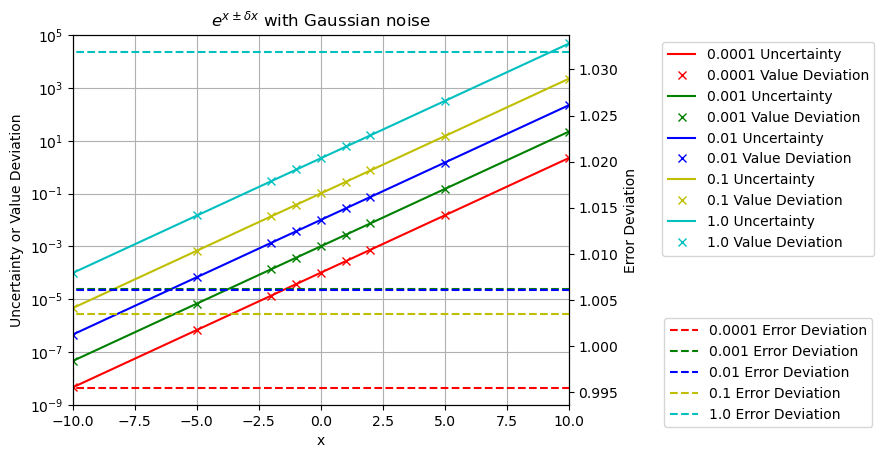
\includegraphics[height=2.5in]{Exp_Dev.png} 
\captionof{figure}{
The calculated uncertainties vs the measured value deviations and the measured error deviations for $e^{x \pm \delta x}$, for different $\delta x$ as shown in the legend.
The uncertainties and the value deviations are drawn using the logarithmic y scales on the left side, while the error deviations are drawn using the linear y scales on the right side. 
Each color represent a $\delta x$.
Gaussian noises are used to produce the input noise $\delta x$.
}
\label{fig: Exp_Dev}
\end{figure}

\begin{figure}[p]
\centering
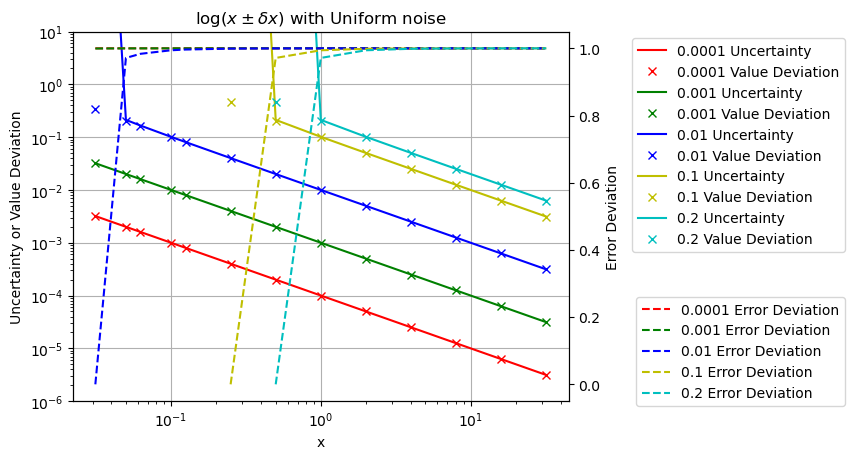
\includegraphics[height=2.5in]{Log_Dev.png} 
\captionof{figure}{
The calculated uncertainties vs the measured value deviations and the measured error deviations for $\log(x \pm \delta x)$, for different $\delta x$ as shown in the legend.
The uncertainties and the value deviations are drawn using the logarithmic y scales on the left side, while the error deviations are drawn using the linear y scales on the right side. 
Each color represent a $\delta x$.
Gaussian noises are used to produce the input noise $\delta x$.
}
\label{fig: Log_Dev}
\end{figure}

\begin{figure}[p]
\centering
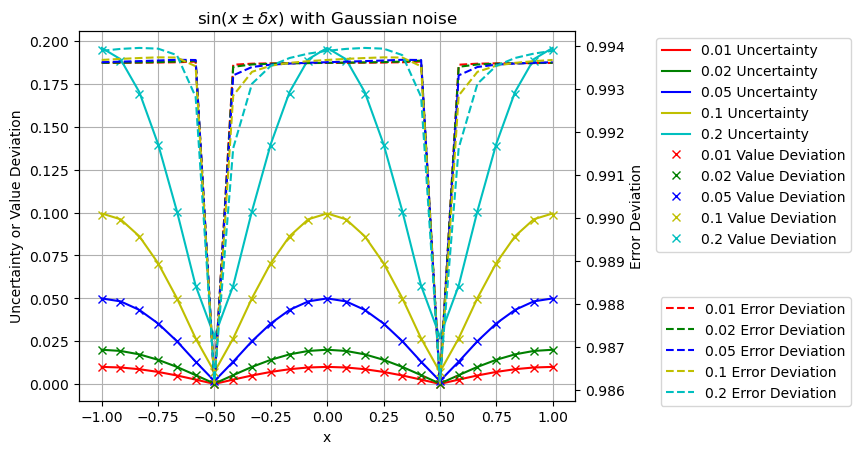
\includegraphics[height=2.5in]{Sin_Dev.png} 
\captionof{figure}{
The calculated uncertainties vs the measured value deviations and the measured error deviations for $\sin(x \pm \delta x)$, for different $\delta x$ as shown in the legend.
The uncertainties and the value deviations are drawn using the logarithmic y scales on the left side, while the error deviations are drawn using the linear y scales on the right side. 
Each color represent a $\delta x$.
Gaussian noises are used to produce the input noise $\delta x$.
}
\label{fig: Sin_Dev}
\end{figure}

\begin{figure}[p]
\centering
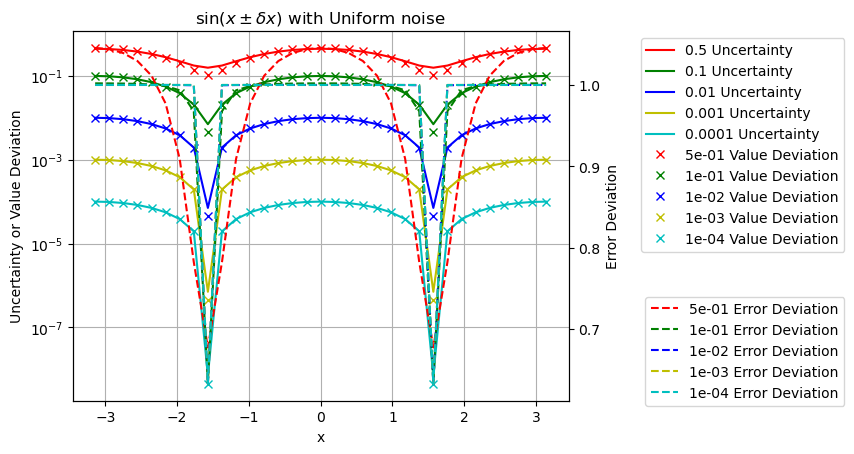
\includegraphics[height=2.5in]{Sin_Dev_Uniform.png} 
\captionof{figure}{
The calculated uncertainties vs the measured value deviations and the measured error deviations for $\sin(x \pm \delta x)$, for different $\delta x$ as shown in the legend.
The uncertainties and the value deviations are drawn using the logarithmic y scales on the left side, while the error deviations are drawn using the linear y scales on the right side. 
Each color represent a $\delta x$.
Uniform noises are used to produce the input noise $\delta x$.
}
\label{fig: Sin_Dev_Uniform}
\end{figure}

\begin{figure}[p]
\centering
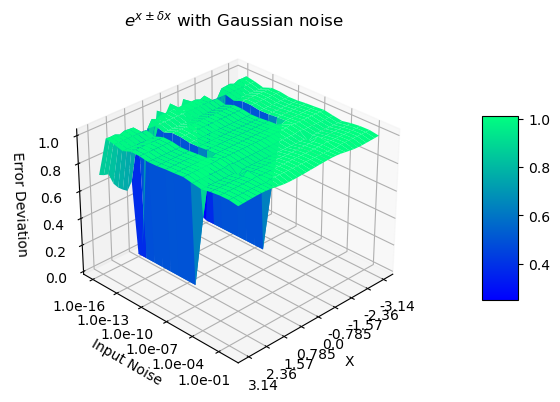
\includegraphics[height=2.5in]{Sin_X_Dev.png} 
\captionof{figure}{
The error deviation for $\sin(x \pm \delta x)$, for $x$ and $\delta$.
The x-axis is $x$ between $-\pi$ and $+\pi$.
The y-axis is $\delta$ between $-10^{-16}$ and $1$.
The z-axis is the error deviation. 
Gaussian noises are used to produce the input noise $\delta x$.
}
\label{fig: Sin_X_Dev}
\end{figure}

\begin{figure}[p]
\centering
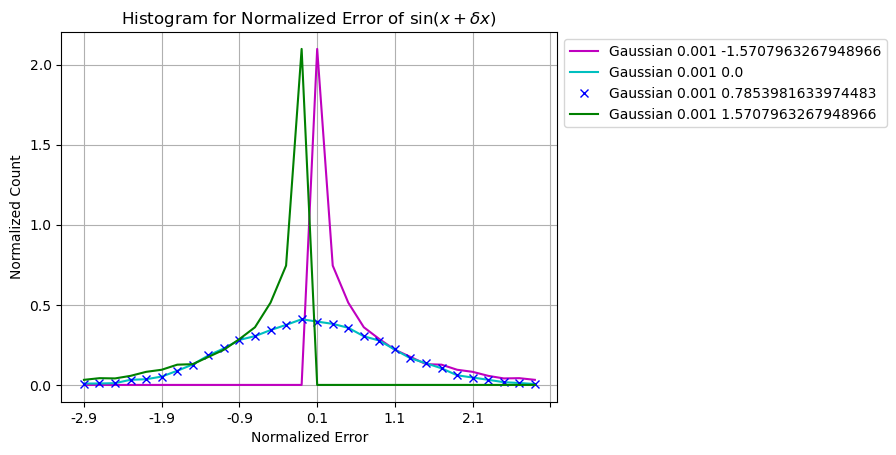
\includegraphics[height=2.5in]{Sin_Histo.png} 
\captionof{figure}{
The histogram of the error deviation for $\sin(x \pm \delta x)$, for $x=-\pi/2, -\pi/4, 0, +\pi/4, +\pi/2$ and $\delta x = 10^{-1}, 10^{-16}$ as shown in the legend.
The y-axis is the normalized count. 
Each color represents a different $x$, while each line pattern represents a different $\delta x$.
Uniform noises are used to produce the input noise $\delta x$.
}
\label{fig: Sin_Histo}
\end{figure}

\begin{figure}[p]
\centering
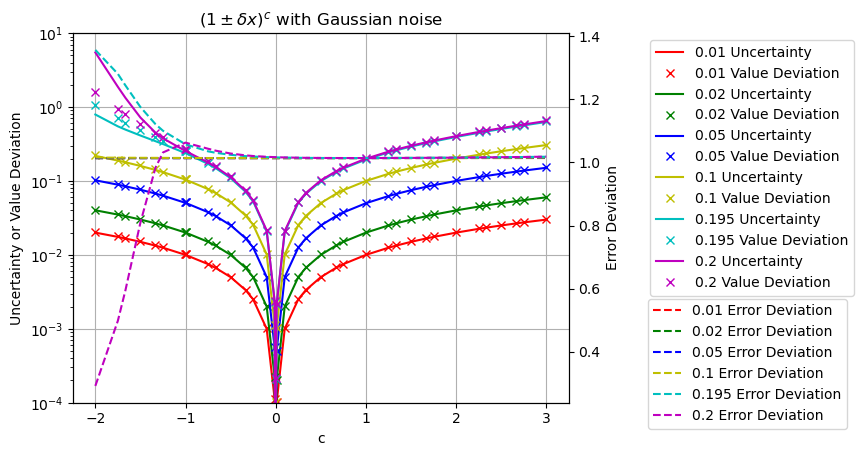
\includegraphics[height=2.5in]{Pow_Dev.png} 
\captionof{figure}{
The calculated uncertainties vs the measured value deviations and the measured error deviations for $(1 \pm \delta x)^c$, for different $\delta x$ as shown in the legend.
The uncertainties and the value deviations are drawn using the logarithmic y scales on the left side, while the error deviations are drawn using the linear y scales on the right side. 
Each color represent a $\delta x$.
}
\label{fig: Pow_Dev}
\end{figure}

\begin{figure}[p]
\centering
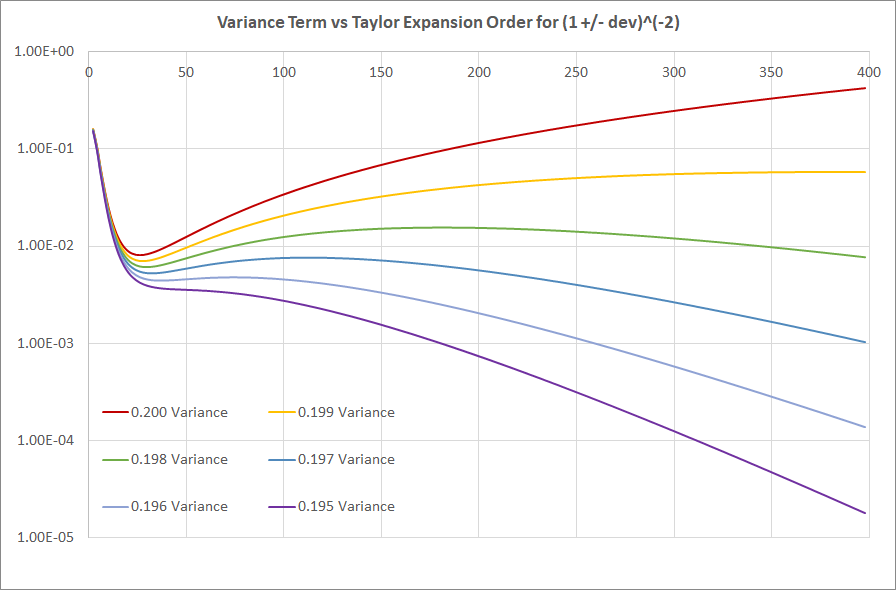
\includegraphics[height=2.5in]{Pow_Converge.png} 
\captionof{figure}{
The individual variance term of $(1 \pm \delta x)^c$ vs the different Taylor expansion order $2n$, for different $c$ and $\delta x$ as shown in the legend. 
The $x$-axis is Taylor expansion order $2n$ from 1 to 400 in Formula \eqref{eqn: Taylor 1d variance}.
The $y$-axis is the contribution to $(1 \pm \delta x)^c$ at each Taylor expansion order $2n$ according to Formula \eqref{eqn: power precision}.
It shows that $(1 \pm 0.2)^{-2}$ and $(1 \pm 0.2)^{-1.5}$ clearly diverge, $(1 \pm 0.2)^{-1}$ seems diverges, and other cases clearly converge.
}
\label{fig: Pow_Converge}
\end{figure}

\begin{figure}[p]
\centering
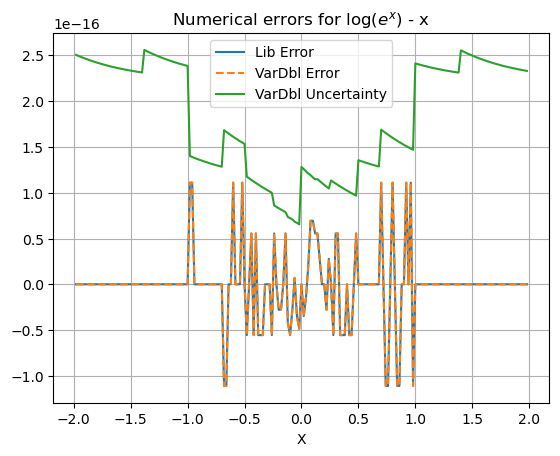
\includegraphics[height=2.5in]{ExpLog_Error.png} 
\captionof{figure}{
The values and uncertainties of $\log(e^x) - x$ vs $x$, as \textit{VarDbl Error} and \textit{VarDbl Uncertainty} in the legend.
The result of the same calculation using conventional floating-point library functions is shown as \textit{Lib Error} in the legend.
}
\label{fig: ExpLog_Error}
\end{figure}

\begin{figure}[p]
\centering
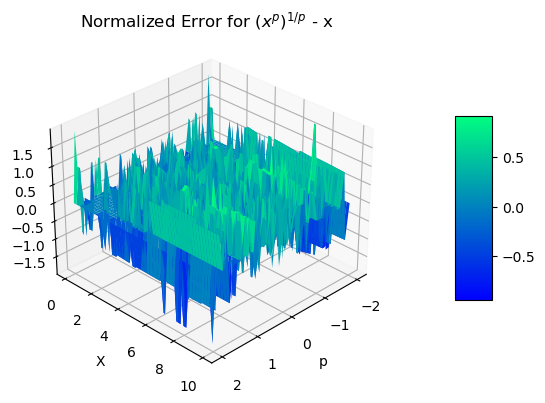
\includegraphics[height=2.5in]{Power_Error.png} 
\captionof{figure}{
The normalized errors of $(x^p)^{\frac{1}{p}} - x$ vs $x$ and $p$.
}
\label{fig: Power_Error}
\end{figure}


Formula \eqref{eqn: exp precision}, \eqref{eqn: log precision}, \eqref{eqn: sin precision}, and \eqref{eqn: power precision} are tested by the corresponding math library functions \textit{exp}, \textit{log}, \textit{sin}, and \textit{pow}, respectively.

At each point $x$ for an input uncertainty $\delta x$, the result uncertainty is calculated by the variance arithmetic.
The corresponding value deviation is obtained by:
\begin{enumerate}

\item Take $10000$ samples from either Gaussian noise or uniform distribution with $\delta x$ as the deviation, and construct $\tilde{x}$ which is $x$ plus the sampled noise.  

\item For each $\tilde{x}$, use the corresponding library function to calculate the value error as the difference between using $\tilde{x}$ and using $x$ as the input.

\item The value error is divided by the result uncertainty, as the normalized error.

\item The standard deviation of the $10000$ normalized errors is the error deviation.

\item In addition, for each of these tests, all value errors follow a same underlying distribution.
The deviation of the value errors is defined as the \emph{value deviation}, which the uncertainty should match.

\end{enumerate}

\subsection{Exponential}

Figure \ref{fig: Exp_Dev} shows that the calculated uncertainties using Formula \eqref{eqn: exp precision} agree very well with the measured value deviations for $e^{x + \delta x}$.
As a result, the error deviations are very close to $1$, even both the uncertainties and the value error deviations increase exponentially with $x$ and $\delta x$.
Such strong tracking power holds for all $x$ of $e^{x + \delta x}$. 

\subsection{Logarithm}

Figure \ref{fig: Log_Dev} shows that the calculated uncertainties using Formula \eqref{eqn: log precision} agree very well with the measured value deviations for $\log(x + \delta x)$, so that the result error deviations are very close to $1$, until the uncertainties suddenly diverge when the input precision is coarser than $1/5$ which is the estimated application precision threshold.
After the result uncertainties diverge, the corresponding value deviations still continue on the same trends until the input data to the $\log$ function start to have negative values whenthe input noises are uniformly distributed.
If Gaussian noises are used instead, the cutoffs for both value errors and error deviations are strictly at $1/5$.
The result probability density function for $\log(x)$ has a pole at $x=0$.

Such divergences of the result uncertainties are expected when the input precision is coarser than the estimated applicable precision threshold of $1/\sigma$, in which $\sigma=5$ is the bonding factor of the variance arithmetic.
If $\sigma$ is reduced from $5$ to $4$, the measured applicable precision thresholds increase from $1/5$ to $1/4$, allowing more result uncertainties to be valid.
The reduction of $\sigma$ increases the bounding leakage $\epsilon$ from $5.7 \times 10^{-7}$ to $6.3 \times 10^{-5}$ according to Formula \eqref{eqn: bounding leakage}.
A large leakage $\epsilon$ raises the logic questions on the validity of the result, because the leakage may mean $x \leq 0$ for $\log(x)$ in this case.
In an extreme approach, in another variance arithmetic representation:
\begin{enumerate}

\item Each imprecise value carries its own $\sigma$ or $\epsilon$ to indicate the statistical significance of its value to its uncertainty.

\item The result $\sigma$ or $\epsilon$ involving two imprecise values can be found statistically.

\item The result of an analytic function always converges but at the expense of $\epsilon$, such that  when $x \rightarrow 0$, $\epsilon \rightarrow 1$ for $\log(x + \delta x)$. 

\item A calculation may branch based on the probability $\epsilon$.

\end{enumerate}
For the discussion simplicity, the cases of the bounding factor $\sigma$ other than constant $5$ are avoided in this paper.




\subsection{Sine}

Figure \ref{fig: Sin_Dev} shows that the calculated uncertainties using Formula \eqref{eqn: sin precision} agree very well with the measured value deviations for $\sin(x + \delta x)$.
Figure \ref{fig: Sin_Dev} also shows that $\delta^2 \sin(x)$ has the same periodicity as $\sin(x)$:
\begin{itemize}
\item When $x=0$, $\sin(x) \simeq x$, so that $\delta^2 \sin(x) \simeq (\delta x)^2$.
\item When $x=\pi/2$, $\sin(x) \simeq 1$, so that $\delta^2 \sin(x) \simeq 0$.
\end{itemize}

In Figure \ref{fig: Sin_Dev}, Gaussian noises are used, while in Figure \ref{fig: Sin_Dev_Uniform}, ideal white noises are added for then given sample size of $10000$.
The difference of Figure \ref{fig: Sin_Dev} and \ref{fig: Sin_Dev_Uniform} shows that the Gaussian noise is more desirable, because of its tail effect, e.g., the error deviation is much closer to $1$ for $\sin(\pm \pi/2 + \delta x)$.
So only Gaussian noises will be used for other analysis by default.

Figure \ref{fig: Sin_X_Dev} shows that the error deviation for $\sin(x + \delta x)$ is $1$ except when $x=\pm \pi/4$ and $\delta x < 10^{-12}$, at where the probability density function has a zero.
Figure \ref{fig: Sin_Histo} shows the histogram of the error deviation for $\sin(x + \delta x)$ when Gaussian noises are used to produce the input noise $\delta x$:
\begin{itemize}
\item When $\delta x=10^{-16}$, the noise is comparable to the numerical calculation error of $\sin(x)$.
The histogram is highly structured, with peaks near $0$, $\pm 1$, and $\pm 2$, suggesting that the value errors are integer-folds of the least significant value.

\item When $\delta x=10^{-1}$, the noise is much large than the numerical calculation error of $\sin(x)$, so that ideal coverage is achieved.
When $x=\pm \pi/2$, $\sin(x)^{(1)}_{x} = 0$, so that the result probability density function has a zero.
The corresponding histogram is distorted from Gaussian, with the peak at $x=\pm \pi/2$, and all other values on one side of the peak only.
Such distortion of the histogram 
\end{itemize}


\subsection{Power}

Figure \ref{fig: Pow_Dev} shows that the calculated uncertainties of $(1 \pm \delta x)^c$ using Formula \eqref{eqn: power precision} agree very well with the measured value deviations for $(1 + \delta x)^c$ except when $\delta x =0.2$ and $c < -1$.
The reason why Formula \eqref{eqn: power precision} is not applicable exactly at the estimated applicable precision threshold $1/\sigma$ needs further discussion.
Figure \ref{fig: Pow_Converge} shows the individual variance term of $(1 \pm \delta x)^c$ for the different Taylor expansion order $2n$, for different $c$ and $\delta x$.
\begin{itemize}

\item Formula \eqref{eqn: inversion precision} and \eqref{eqn: inversion square precision} show that $(1 \pm 0.2)^{-2}$ diverges faster than $(1 \pm 0.2)^{-1}$, which is confirmed by both Figure \ref{fig: Pow_Dev} and \ref{fig: Pow_Converge}.

\item 
When the deviation is reduced slightly to below $1/\sigma$ from $0.2$ to $0.195$, Figure \ref{fig: Pow_Dev} shows that the error deviations become much closer to $1$.  
As the confirmation, Figure \ref{fig: Pow_Converge} shows reducing $\delta x$ increases the convergence, e.g., $(1 \pm 0.2)^{-1.5}$ diverges while $(1 \pm 0.195)^{-2}$ converges.

\item Figure \ref{fig: Pow_Dev} and \ref{fig: Pow_Converge} shows that the convergence is more sensitive to $\delta x$ than $c$, so that the applicable precision threshold is relatively hard, which is estimated as $\delta x = 0.196$ for $c=-2$.

\end{itemize}
Figure \ref{fig: Pow_Converge} shows that the convergence of an analytic function at each input can be judged numerically and automatically for the given maximum Taylor expansion orders.



\subsection{Numerical Errors for Library Functions}

The combined numerical error of the library function $e^x$ and $\log(x)$ is calculated as $\log(e^x) - x$ vs $x$.
Figure \ref{fig: ExpLog_Error} shows that using either the variance arithmetic or the conventional floating-point library functions results in the same value errors.  
In both cases, the value errors are $0$ when $1 < |x|$.
The uncertainties of the variance arithmetic bounds the value errors effectively, resulting in an error deviation about $0.409$ when $|x| \leq 1$.

The numerical error of the library function $x^p$ is calculated as $(x^p)^{1/p} - x$ vs $x$.
Figure \ref{fig: Power_Error} shows that the normalized errors is not specific to either $x$ or $p$, resulting in an error deviation about $0.548$.

When no input noise is added, the error deviation of $\sin(x)^2 + \cos(x)^2 - 1$ is about $0.535$


\subsection{Summary}

Formula \eqref{eqn: exp precision}, \eqref{eqn: log precision}, \eqref{eqn: sin precision}, and \eqref{eqn: power precision} gives effective uncertainties for the corresponding library functions.
Generally, when the input precision is above $10^{-15}$, the input uncertainty achieves ideal coverage.

In ideal coverage cases, the error deviation is very close to $1$ except it is $0$ at where:
\begin{itemize}
\item when the result probability density function is zero, and $\delta x$ is small enough, the uncertainty mean is finite.

\item when the result probability density function is pole, and $\delta x$ is large enough, the uncertainty mean is infinite.
\end{itemize}
In non ideal coverage cases, the error deviation is about $0.5$.





\clearpage
\section{Regressive Generation of Sin/Cos}
\label{sec: recursion}

\begin{figure}
\centering
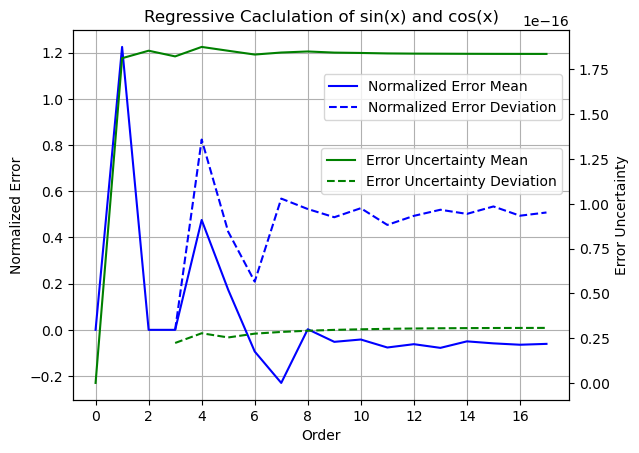
\includegraphics[height=2.5in]{Uncertain_Sin.png} 
\captionof{figure}{
The error deviations and uncertainty means for $\sin(x)^2 + \cos(x)^2 - 1, x \in [0, \pi/4]$, for different regression order as shown in the legend.
}
\label{fig: Uncertain_Sin}
\end{figure}

Starting from Formula \eqref{eqn: phase boundary}, Formula \eqref{eqn: phase sin} and Formula \eqref{eqn: phase cos} can be used recursively to calculate the $\sin$ library function.  
\begin{align}
\label{eqn: phase boundary}
& \sin(0) = \cos(\frac{\pi}{2}) = 0; & \sin(\frac{\pi}{2}) = \cos(0) = 1; \\
\label{eqn: phase sin}
& \sin \left(\frac{\alpha + \beta}{2} \right) = \sqrt{\frac{1 - \cos \left(\alpha + \beta \right)}{2}} = & \sqrt{\frac{1 - \cos(\alpha) \cos \left(\beta) + \sin(\alpha \right) \sin(\beta)}{2}}; \\
\label{eqn: phase cos}
& \cos \left(\frac{\alpha + \beta}{2} \right) = \sqrt{\frac{1 + \cos \left(\alpha + \beta \right)}{2}} = & \sqrt{\frac{1 + \cos(\alpha) \cos(\beta) - \sin(\alpha) \sin(\beta)}{2}};
\end{align}
The number of regression is defined as the order.
For each order $n$, $2^n$ $\sin(\frac{\pi}{2} \frac{i}{2^n})$ and $\cos(\frac{\pi}{2} \frac{i}{2^n})$ values are obtained, so that the result is more statistically stable with increasing $n$.

The errors of the generated $\sin(x)$ and $\cos(x)$ are checked by $\sin(x)^2 + \cos(x)^2 - 1$.
The resulted value errors are very comparable with the value errors using floating-point library $\sin(x)$ and $\cos(x)$.
Figure \ref{fig: Uncertain_Sin} shows that the result uncertainties remain almost a constant of about $1.2 \time 10^{-16}$, which is consist with uniformly distributed least significant values within the least significant bit of the significand.
It also shows that the error deviations is close to $0.5$, which is comparable to the value of $0.535$ for the library $\sin(x)$ and $\cos(x)$ functions.

The variance arithmetic is thus effective for this regression algorithm.




\clearpage
\section{Verification Using FFT}
\label{sec: FFT}


\subsection{Unfaithful Frequency Response of Discrete Fourier Transformation \cite{Prev_Precision_Arithmetic}}

\iffalse

The Fourier transformation of a linear signal $h[n] = n$. 
Let $y \equiv i 2\pi n /N$:
\begin{align*}
& G(y) = \sum_{k=0}^{N-1}  e^{y k} = \sum_{k=0}^{N-1}  (e^y)^k = \frac{e^{N y} - 1}{e^y - 1}
 = \begin{cases} y = 0: \eqspace N \\ y \neq 0: \eqspace 0 \end{cases}; \\
H[n] &= \sum_{k=0}^{N-1} k e^{\frac{i 2\pi n}{N} k} = \sum_{k=0}^{N-1} k e^{y k} 
 = \frac{d G}{y} = \frac{N e^{N y}}{e^y - 1} - \frac{e^{N y} - 1}{(e^y - 1)^2} e^y = \frac{N}{e^y - 1} \\
 &= \frac{N}{\cos(y) - 1 + i \sin(y)} = \frac{N}{2} \frac{\cos(y) - 1 -  i \sin(y)}{1 - \cos(y)} 
  = - \frac{N}{2}(1 + i \frac{2 \sin(\frac{y}{2}) \cos(\frac{y}{2})}{2 \sin^2(\frac{y}{2})}) \\
 &= \begin{cases} y = 0: \eqspace \frac{N^2}{2} \\ y \neq 0: \eqspace - \frac{N}{2}(1 + i \frac{1}{\tan(\frac{n}{N} \pi)}) \end{cases};
\end{align*}

\fi

\begin{figure}%[p]
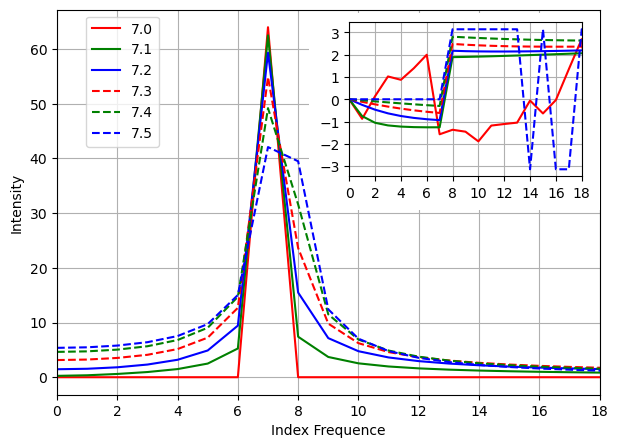
\includegraphics[width=4.5in,height=2.75in]{FFT_Unfaithful.png} 
\captionof{figure}{An unfaithful Discrete Fourier transformation is demonstrated by the spectra of a few sine signals having amplitude of 1 and slightly different frequencies as shown in legends..  
This figure is a practical reproduction of a previous theoretical figure \cite{Prev_Precision_Arithmetic}.
}
\label{fig: FFT_Unfaithful}
\end{figure}

Each testing algorithm needs to come under careful scrutiny.  
One important issue is whether the digital implementation of the algorithm is faithful for the original analytic algorithm.  
For example, the discrete Fourier transformation is only faithful for Fourier transformation at certain frequencies, and it has a different degree of faithfulness for other frequencies.  
This is called the \emph{unfaithful frequency response} of the discrete Fourier transformation.

For each signal sequence $h[k], k = 0, 1 \dots  N-1$, in which $N$ is a positive integer, the discrete Fourier transformation $H[n], n = 0, 1 \dots  N-1$ and its reverse transformation is given by Formula \eqref{eqn: Fourier} \cite{Numerical_Recipes}, in which $k$ is the \emph{index frequency} for the discrete Fourier transformation:
\begin{align}
\label{eqn: Fourier}
& H[n]=\sum_{k=0}^{N-1}h[k] \; e^{i 2\pi \frac{k}{N} n};
& h[k]=\frac{1}{N} \sum_{n=0}^{N-1}H[n] \; e^{-i 2\pi \frac{n}{N} k};
\end{align}

The $H[n]$ of a pure sine signal $h[k] = \sin \left(2\pi f k/N \right)$ is calculated by Formula \eqref{eqn: sin Fourier}, in which $f$ is the frequency of the sine wave.  
The solution for Formula \eqref{eqn: sin Fourier} is Formula \eqref{eqn: sin Fourier solution}, which transform the sine signal to a delta-like function with $\pi/2$ as phase only when $f$ is an integer between $0$ and $N/2$.
In other cases, how much the result of discrete Fourier transformation deviates from continuous Fourier transformation depends on how much $f$ deviates from an integer, e.g., when $f$ is exactly between two integers, the phase of the transformation is that of cosine instead of sine according to Formula \eqref{eqn: sin Fourier solution}.
Examples of unfaithful representations of fractional frequency by the discrete Fourier transformation are shown in Figure \ref{fig: FFT_Unfaithful}. 
The data for Figure \ref{fig: FFT_Unfaithful} is generated using \textit{SciPy}, which are very reproducible using any other math libraries, including \textit{MathLab} and \textit{Mathematica}.
\begin{align}
\centering
\label{eqn: sin Fourier}
H[n] &= \frac{1}{2 i}\left( \sum_{k=0}^{N-1}e^{i 2\pi (n+f)\frac{k}{N}}  - \sum_{k=0}^{N-1} e^{i 2\pi (n-f)\frac{k}{N}} \right) \\
\label{eqn: sin Fourier solution}
&= \begin{cases}
  i N/2, & f \text{ is integer} \\
  N/\pi, & f \text{ is integer} + 1/2 \\
  \frac{1}{2} \frac{\sin(2\pi f - 2\pi \frac{f}{N}) + \sin(2\pi \frac{f}{N})-\sin(2\pi f) e^{-i 2\pi \frac{n}{N}}}{\cos(2\pi \frac{n}{N})-\cos(2\pi \frac{f}{N})} & \text{otherwise}
\end{cases}
\end{align}

Due to its width, a frequency component in an unfaithful transformation may interact with other frequency components of the Discrete Fourier spectrum, thus sabotaging the whole idea of using the Fourier Transformation to decompose a signal into independent frequency components.  
Because the reverse discrete Fourier transformation mathematically restores the original $\{h[k]\}$ for any $\{H[n]\}$, it exaggerates and narrows all unfaithful signal components correspondingly.  
This means that the common method of signal processing in the Fourier space \cite{Numerical_Recipes}\cite{Stochastic_Arithmetic}\cite{Floating-point_Digital_Filters} may generate artifacts due to its uniform treatment of faithful and unfaithful signal components, which probably coexist in reality.  
Unlike aliasing \cite{Electronics}\cite{Numerical_Recipes}\cite{Floating-point_Digital_Filters}, unfaithful representation of the discrete Fourier transformation has an equal presence in the whole frequency range so that it cannot be avoided by sampling the original signal differently.

An unfaithful representation arises from the implied assumption of the discrete Fourier transformation.  
The continuous Fourier transformation has an infinitive signal range so that:
\begin{equation}
\label{eqn: Fourier continuous shift}
h(t) \Leftrightarrow H(s): \eqspace h(t - \tau) \Leftrightarrow H(s) e^{i 2\pi s \tau};
\end{equation}
As an analog, the discrete Fourier transformation $G[n]$ of the signal $h[k], k = 1 \dots N$ can be calculated mathematically from the discrete Fourier transformation $H[n]$ of $h[k], k = 0\dots N-1$:
\begin{equation}
\label{eqn: Fourier discrete shift}
G[n] = (H[n] + h[N] - h[0]) e^{i 2\pi n/N};
\end{equation}
Applying Formula \eqref{eqn: Fourier continuous shift} to Formula \eqref{eqn: Fourier discrete shift} results in Formula \eqref{eqn: Fourier discrete assumption}.
\begin{equation}
\label{eqn: Fourier discrete assumption}
h[N] = h[0];
\end{equation}
Thus, the discrete Fourier transformation has an implied assumption that the signal $h[k]$ repeats itself outside the region of $[0, N-1]$ \cite{Numerical_DFT}.  
For an unfaithful frequency, $h[N-1]$ and $h[N]$ are discontinuous in regard to signal periodicity, resulting in larger peak width, lower peak height, and the wrong phase.  

The unfaithfulness of the discrete Fourier transformation to the Fourier transformation is a very serious example of modeling errors, but this problem has not be addressed seriously enough previously.
Because the discrete Fourier transformation has widest applications in science and engineering, this problem really need some serious attention.



\subsection{Testing Signals}

To avoid the unfaithful representation, the validation of the variance arithmetic using discrete Fourier transformation will not rely on the ideal result from the continuous Fourier transformation counterpart.
Instead, the analytic result will be calculated using only Formula \eqref{eqn: Fourier}.

The following signals are used for testing:
\begin{itemize}
\item \emph{Sin}: $h(n) = \sin(n \frac{2\pi f}{N}), f = 1, 2, ... N/2 -1$, in which $f$ is defined as the \emph{index frequency}.

\item \emph{Cos}: $h(n) = \cos(n \frac{2\pi f}{N}), f = 1, 2, ... N/2 -1$, in which $f$ is the index frequency.

\item \emph{Linear}: $h[n] = n$, whose discrete Fourier transformation is Formula \eqref{eqn: Fourier spec for linear}.
\begin{align}
& y \equiv i 2\pi \frac{n}{N}: \eqspace G(y) = \sum_{k=0}^{N-1}  e^{y k} = \frac{e^{N y} - 1}{e^y - 1}
 = \begin{cases} y = 0: \eqspace N \\ y \neq 0: \eqspace 0 \end{cases}; \nonumber \\
\label{eqn: Fourier spec for linear}
H[n] &= \frac{d G}{d y} = \begin{cases} n = 0: \eqspace \frac{N (N-1)}{2} \\ n \neq 0: \eqspace - \frac{N}{2}(1 + i /\tan(n \frac{\pi}{N})) \end{cases};
\end{align}

\end{itemize}

Empirically:
\begin{itemize}
\item The results from Sin/Cos are statistically indistinguishable from each other.

\item The results from Sin at different frequencies are statistically indistinguishable from each other.
\end{itemize}
So the results for Sin/Cos signals at all frequencies are pooled together for the statistical analysis, as the \emph{Sin/Cos} signals.


\subsection{FFT (Fast Fourier Transformation)}

\iffalse

Forward:
\begin{align*}
L = 1:\;& o=0: & [0, 1]; \\
 & o = 1: & F = [0 + 1, 0 - 1]; \\
L = 2:\;& o=0: & [0, 2, 1, 3]; \\
 & o = 1: & [0 + 2, 0 - 2, 1 + 3, 1 - 3]; \\
 & o = 2: & [0 + 1 + 2 + 3, 0 + i 1 - 2 - i 3 , 0 - 1 + 2 - 3, 0 - i 1 - 2 + i 3; \\
 & [0, 1, 0, -1]:& [0, i 2, 0, - i 2]; \\
 & [1, 0, -1, 0]:& [0, 2, 0, 2];
\end{align*}

Reverse:
\begin{align*}
L = 1:\;& o=0: & [0, 1]; \\
 & o = 1: & F = [0 + 1, 0 - 1]; \\
L = 2:\;& o=0: & [0, 2, 1, 3]; \\
 & o = 1: & [0 + 2, 0 - 2, 1 + 3, 1 - 3]; \\
 & o = 2: & [0 + 1 + 2 + 3, 0 - i 1 - 2 + i 3 , 0 - 1 + 2 - 3, 0 + i 1 - 2 - i 3; \\
 & [0, i 2, 0, - i 2]:& [0, 4, 0, -4]; \\
 & [0, 2, 0, 2]:& [4, 0, -4, 0];
\end{align*}

\fi

When $N = 2^{L}$, in which $L$ is a positive integer, the generalized Danielson-Lanczos lemma \cite{Numerical_Recipes} can be applied to the discrete Fourier transformation as FFT \cite{Numerical_Recipes}. 
\begin{itemize}

\item For each output, each input is only used once, so there is no dependency problem when using Formula \eqref{eqn: addition and subtraction} and \eqref{eqn: multiplication} as arithmetic operations.
This simplicity avoids introducing numerical errors from Formula \eqref{eqn: Taylor 1d variance}, because $f^{(j)}_x$ may contain numerical errors, while $(\delta x)^{2n}$ may contain rounding errors.

\item When $L$ is large, the large amount of input and output data enables high quality statistical analysis.

\item The amount of calculation is $L$, because for each output, increasing $L$ by 1 results in one additional step of sum of multiplication.

\item Each step in the forward transformation thus increase the variance by $2$-fold, so that the result uncertainty means increase with the FFT order $L$ as $\sqrt{2}^L$.
Because the reverse transformation divides the result by $2^L$, the result uncertainty means decrease with the FFT order $L$ as $\sqrt{1/2}^L$.
The result uncertainty means for the roundtrip transformations is thus: $\sqrt{2}^L \times \sqrt{1/2}^L = 1$.

\item The major source of the calculation error for Sin/Cos signals is the calculation errors of the library function $\sin(\pi j /2^L), j = 0, 1, 2 ... 2^{L-1}$.
The major source of the calculation error for \emph{Linear} signals is the calculation errors of the library function $\tan(\pi (j - 1) /2^L), j = 1, 2 ... 2^{L-1}$.

\item The forward and reverse transformations are identical except a sign, so they are essentially the same algorithm, and their difference is purely due to input data.  

\item The forward transformation cancels each datum of a Sin/Cos signal into a spectrum of mostly $0$ values, while the reverse transformation spread the spectrum of mostly $0$ values to each datum of a Sin/Cos signal, so their data have contrast nature.

\end{itemize}


\subsection{Ideal Coverage}

\begin{figure}[p]
\centering
\includegraphics[height=2.5in]{FFT_SinCos_vs_Noise.png} 
\captionof{figure}{
The result error deviations and uncertainty means using Sin/Cos signals of order 18 vs. input uncertainties for forward, reverse and roundtrip FFT transformations.
The error deviations are scaled to the linear y-axis on the right, while the uncertainty means are scaled to the logarithmic log y-axis on the right.
}
\label{fig: FFT_SinCos_vs_Noise}
\end{figure}

\begin{figure}[p]
\centering
\includegraphics[height=2.5in]{FFT_Linear_vs_Noise.png} 
\captionof{figure}{
The result error deviations and uncertainty means using Linear signals of order 18 vs. input uncertainties for forward, reverse and roundtrip FFT transformations.
The error deviations are scaled to the linear y-axis on the right, while the uncertainty means are scaled to the logarithmic log y-axis on the right.
}
\label{fig: FFT_Linear_vs_Noise}
\end{figure}

\begin{figure}[p]
\centering
\includegraphics[height=2.5in]{FFT_SinCos_1e-12_vs_Order.png} 
\captionof{figure}{
The result error deviations and uncertainty means using Sin/Cos signals with $10^{12}$ noises vs. FFT order for forward, reverse and roundtrip FFT transformations.
The error deviations are scaled to the linear y-axis on the left, while the uncertainty means are scaled to the logarithmic log y-axis on the right.
}
\label{fig: FFT_SinCos_1e-12_vs_Order}
\end{figure}

\begin{figure}[p]
\centering
\includegraphics[height=2.5in]{FFT_Linear_1e-5_vs_Order.png} 
\captionof{figure}{
The result error deviations and uncertainty means using Lienar signals with $10^{5}$ noises vs. FFT order for forward, reverse and roundtrip FFT transformations.
The error deviations are scaled to the linear y-axis on the left, while the uncertainty means are scaled to the logarithmic log y-axis on the right.
}
\label{fig: FFT_Linear_1e-5_vs_Order}
\end{figure}


Figure \ref{fig:  FFT_SinCos_vs_Noise}  shows the result error deviations and uncertainty means vs. different input uncertainties using Sin/Cos signals of order 18.  
When the deviation of the input noise is more than $10^{-12}$, the input uncertainties become ideal coverage:
\begin{itemize}
\item As expected, the normalized errors for the forward and the reverse transformations are normal distributed, even when the input noise is no longer Gaussian.
The normalized errors for the roundtrip transformations are delta distributed at $0$.

\item As expected, the result uncertainty means for the roundtrip transformation recover the corresponding input uncertainties perfectly. 
The result uncertainty means for both the forward and the reverse transformations are linear to the input uncertainties, respectively, because FFT transformations are linear.

\item For the roundtrip transformations, the result is compared with the original input for value errors, which are virtually $0$.
The corresponding error deviations are also $0$, and the normalized errors are delta distributed at $0$.

\end{itemize}
Figure \ref{fig: FFT_Linear_vs_Noise} is identical to Figure \ref{fig: FFT_SinCos_vs_Noise} except that the ideal coverage is reached when the input noise deviation is $10^{-3}$ or more.

Figure \ref{fig:  FFT_SinCos_1e-12_vs_Order}  shows the result error deviations and uncertainty means vs. FFT order using Sin/Cos signals with $10^{-12}$ noise, when the input uncertainties start to have idea coverage over the input errors.
\begin{itemize}
\item The result uncertainty means for the forward transformations increase with the FFT order $L$ as $\sqrt{2}^L$, as expected.

\item The result uncertainty means for the reverse transformations decrease with the FFT order $L$ as $\sqrt{1/2}^L$, as expected.

\item The result uncertainty means for the roundtrip transformations always equal the corresponding input uncertainties, as expected.

\item The result error deviations for the the forward and the reverse transformations are exactly constant $1$ when the FFT order is more than $10$.
Smaller FFT order probably means not enough samples for the error deviations to reach stable values.
\end{itemize}
Such trends of uncertainty means are observed for all cases of ideal coverage.

Figure \ref{fig:  FFT_Linear_1e-5_vs_Order}  shows the result error deviations and uncertainty means vs. FFT order using Linear signals with $10^{-5}$ noises, when the input uncertainties are below the ideal coverage of $10^{-3}$.
The result uncertainty means have the behaviors as if the ideal coverage has been reached.
The result error deviations reach exactly constant $1$ between the FFT order $12$ and $16$ but deviate from $1$ when the FFT order is more than $16$, because more calculations bring more numerical errors from the $\tan$ library functions.
This means a test calculation of smaller scale may behaves quite different from a real calculation in term of result error characteristics.

For both signals, FFT transformations are validated for ideal coverage.
Both error response and calculation response have the expected behaviors, the result normalized errors are normal distributed, and the error deviations are exactly $1$.




\subsection{Non Ideal Coverage}

\begin{figure}[p]
\centering
\includegraphics[height=2.5in]{FFT_SinCos_Clean_vs_Order.png} 
\captionof{figure}{
The result error deviations and uncertainty means using Sin/Cos signals vs. FFT order for forward, reverse and roundtrip FFT transformations, as shown in the legend.
The error deviations are scaled to the linear y-axis on the left, while the uncertainty means are scaled to the logarithmic log y-axis on the right.
}
\label{fig: FFT_SinCos_Clean_vs_Order}
\end{figure}

\begin{figure}[p]
\centering
\includegraphics[height=2.5in]{FFT_Sin_Order7_Freq15_Spec_Clean.png} 
\captionof{figure}{
The real and imaginary absolute value errors and uncertainties in the FFT spectrum of a clean Sin signal of order 6 and index frequency 7, as shown in the legend, in which "Error' means value error.
}
\label{fig: FFT_Sin_Order7_Freq15_Spec_Clean}
\end{figure}

\begin{figure}[p]
\centering
\includegraphics[height=2.5in]{FFT_Sin_Error_Histogram.png} 
\captionof{figure}{
The histograms of the normalized errors of Sin/Cos signals at FFT with $10^{-15}$ white noises for forward, reverse and roundtrip FFT transformations, as shown in the legend.
}
\label{fig: FFT_Sin_Error_Histogram}
\end{figure}

\begin{figure}[p]
\centering
\includegraphics[height=2.5in]{FFT_Linear_Clean_vs_Order.png} 
\captionof{figure}{
The result error deviations and uncertainty means using Linear signals vs. FFT order for forward, reverse and roundtrip FFT transformations, as shown in the legend.
The error deviations are scaled to the linear y-axis on the left, while the uncertainty means are scaled to the logarithmic log y-axis on the right.
}
\label{fig: FFT_Linear_Clean_vs_Order}
\end{figure}



Figure \ref{fig: FFT_SinCos_Clean_vs_Order} shows the result uncertainty means and error deviations for forward, reverse and roundtrip FFT transformations on Sin/Cos signals without added noises vs. FFT order $L$.
The trends of the uncertainty means with the FFT order agree with the different natures of the forward, reverse and roundtrip FFT transformations on Sin/Cos signals:
\begin{itemize}
\item For the forward transformations, the uncertainty means increase exponentially as $1.36^L$ with the FFT order $L$.

\item For the reverse transformations, the uncertainty means remain almost a constant about $1.4 \times 10^{-16}$ with the FFT order $L$.

\item For the roundtrip transformations, the uncertainty means remain almost a constant about $1.7 \times 10^{-16}$ with the FFT order $L$.

\end{itemize}

The error deviations are between $0.42$ and $1.21$, confirming the tracking power of the variance arithmetic.
The reason why they are not constant $1$ is attributed to the numerical errors in the library function $\sin(\pi j /2^L), j = 0, 1, 2 ... 2^{L-1}$:
\begin{enumerate}
\item The variance arithmetic can not account for numerical errors in the $\sin$ library function, which will probably increase with the FFT order $L$.
It is probably the reason why the error deviations of the reverse transformation increase slowly with $L$ as $0.0322 L$.

\item Figure \ref{fig: FFT_Sin_Order7_Freq15_Spec_Clean} shows how the variance arithmetic uses uncertainties to track the value errors in a FFT spectrum of a Sin signal with index frequency $7$ and FFT order $7$.
The two peaks of the value errors at the index frequencies $\pm 7$ are expected, but Figure \ref{fig: FFT_Sin_Order7_Freq15_Spec_Clean} also shows a few other large peaks, suggesting systematic errors from the $\sin$ library function.

\item To overcome such systematic errors, $10^{-16}$ white noises are added to the Sin signal.
The result corresponding FFT spectrum looks no longer structured. 
Figure \ref{fig: FFT_Sin_Error_Histogram} confirms that the normalized errors for the forward transformation are normal distributed.

\item In Figure \ref{fig: FFT_Sin_Error_Histogram}, the normalized errors for the reverse transformation are still not normal distributed, and the corresponding error deviations still increase with the FFT order $L$ as $0.0262 L$.
When $10^{-12}$ white noises are added to the Sin signal, for the reverse transformation, the normalized errors become a constant of $1$, and the normalized errors become normal distributed.

\item In the above steps, the noises are only added to the Sin signal.
If instead $10^{-15}$ white noises are added to the sin library function which is also used to generate the Sin/Cos signals, the result error deviations remain near $1$ for the reverse transformation.
Thus, the library function $\sin(x), x \in [0, \pi/2]$ is estimated to contain $10^{-15}$ numerical errors.

\item The structured histogram for the reverse transformation in Figure \ref{fig: FFT_Sin_Error_Histogram} can be used as the signature of the numerical errors on the background of the $10^{-16}$ Gaussian noise.

\end{enumerate}

Figure \ref{fig: FFT_Linear_Clean_vs_Order} shows the result uncertainty means and error deviations for forward, reverse and roundtrip FFT transformations on Linear signals vs. FFT order $L$.
Linear signals contain the $\tan$ library function in Formula \eqref{eqn: Fourier spec for linear}.
Unlike $\sin(x)$, $\tan(x)$ is not bounded and increase with $L$, e.g., for order $18$, the maximal $\tan$ value is $4.78 \times 10^6$, whose least significant value is about $10^{-10}$, which is larger that $10^{-16}$ for the maximal $\sin$ value.
The addition of the new numerical errors from the $\tan$ library function has noticeable impact:
\begin{itemize}
\item The uncertainty means of the forward transformation of Linear signals increase faster exponentially with the FFT order $L$: $2.88^L$ vs $1.42^L$.

\item Because the FFT spectra no longer contain mostly $0$ values, the uncertainty means of the reverse transformation of Linear signals also increase noticeably exponentially with the FFT order $L$: $2.04^L$ vs $1.03^L$.

\item The uncertainty means of the roundtrip transformation increase noticeably exponentially with the FFT order $L$: $2.09^L$ vs $1.04^L$.  
This suggests that the roundtrip transformation can not recover the original input uncertainties.

\item All error deviations are different noticeably from $1$ but still near $1$. 

\item For the order $18$ reverse transformations, $10^{-3}$ input noises are necessary for the result error deviation to be 1 and the result value errors to be normal distributed, which is proportional to the $10^{-12}$ input noise necessary for the Sin/Cos signals.
\end{itemize}

The numerical errors in the library functions cause the input uncertainty converge to be non-ideal.
In the cases of non-ideal coverage:
\begin{itemize}
\item The output is very sensitive to the input data, such as the Sin/Cos signals vs the Linear signals, or the forward transformations vs the reverse transformation.

\item The seemly small uncovered errors may have large impacts on the result: For the reverse transformation, $10^{-15}$ $\sin$ errors are equivalent to $10^{-12}$ input errors, and $10^{-1w}$ $\tan$ errors are equivalent to $10^{-3}$ input error.
\end{itemize}

For both signals, FFT transformations are validated for non ideal coverage.
The result normalized errors are not normal distributed, and the error deviations are near $1$ but probably not exactly $1$.




\subsection{The Need for Ideal Coverage}

\begin{figure}[p]
\centering
\includegraphics[height=2.5in]{FFT_Linear_Forward_ErrorDev_vs_Noise_Order.png} 
\captionof{figure}{
The result error deviations using Linear signals vs. input uncertainties and FFT Orders for the forward transformations.
The input uncertainties run from $10^{-16}$ to $10^{-1}$, while the FFT Order runs from $4$ to $18$.
}
\label{fig: FFT_Linear_Forward_ErrorDev_vs_Noise_Order}
\end{figure}

\begin{figure}[p]
\centering
\includegraphics[height=2.5in]{FFT_Slope_Forward_ErrorDev_vs_Noise_Order.png} 
\captionof{figure}{
The result error deviations using Slope signals vs. input uncertainties and FFT Orders for the forward transformations.
The input uncertainties run from $10^{-16}$ to $10^{-1}$, while the FFT Order runs from $4$ to $18$.
A Slope signal is constructed by replacing $\tan(n \frac{\pi}{N})$ in Formula \eqref{eqn: Fourier spec for linear} with $\frac{\sin(n \frac{2\pi}{2N})}{\sin(n \frac{2\pi}{2N} + \frac{\pi}{2})}$ for the corresponding Linear signal.
}
\label{fig: FFT_Slope_Forward_ErrorDev_vs_Noise_Order}
\end{figure}

\begin{figure}[p]
\centering
\includegraphics[height=2.5in]{FFT_Linear_Reverse_ErrorDev_vs_Noise_Order.png} 
\captionof{figure}{
The result error deviations using Linear signals vs. input uncertainties and FFT Orders for the reverse transformations.
The input uncertainties run from $10^{-16}$ to $10^{-1}$, while the FFT Order runs from $4$ to $18$.
}
\label{fig: FFT_Linear_Reverse_ErrorDev_vs_Noise_Order}
\end{figure}

\begin{figure}[p]
\centering
\includegraphics[height=2.5in]{FFT_Slope_Reverse_ErrorDev_vs_Noise_Order.png} 
\captionof{figure}{
The result error deviations using Slope signals vs. input uncertainties and FFT Orders for the reverse transformations.
The input uncertainties run from $10^{-16}$ to $10^{-1}$, while the FFT Order runs from $4$ to $18$.
A Slope signal is constructed by replacing $\tan(n \frac{\pi}{N})$ in Formula \eqref{eqn: Fourier spec for linear} with $\frac{\sin(n \frac{2\pi}{2N})}{\sin(n \frac{2\pi}{2N} + \frac{\pi}{2})}$ for the corresponding Linear signal.
}
\label{fig: FFT_Slope_Reverse_ErrorDev_vs_Noise_Order}
\end{figure}



Figure \ref{fig: FFT_Linear_Forward_ErrorDev_vs_Noise_Order} and \ref{fig: FFT_Linear_Reverse_ErrorDev_vs_Noise_Order} show the overall dependency of error deviations to both input uncertainties and FFT orders for either the forward or the reverse transform of Linear signals, respectively.
Figure \ref{fig: FFT_Linear_1e-5_vs_Order} is the cross sections along the FFT orders at $10^{-5}$ noise, while Figure \ref{fig: FFT_Linear_vs_Noise} is the cross sections along the input uncertainties at FFT order of $18$.
Both figures shows the ideal coverage as the triangular plains when the error deviations are constant $1$.
Both have steep transitions toward areas of non ideal coverage.
However, for the forward transformations, the transition is a cliff toward a flat valley, while it is a cliff toward a rough mountain.
Also, the ideal coverage plain of the reverse transformation is smaller, and it is expected to disappear when the FFT order is more than $20$ for all input uncertainties.
Figure \ref{fig: FFT_Linear_Forward_ErrorDev_vs_Noise_Order} and \ref{fig: FFT_Linear_Reverse_ErrorDev_vs_Noise_Order} demonstrate the complicity when non ideal coverage presents.

One way to reduce the numerical errors in Linear signals is to replace $\tan(n \frac{\pi}{N})$ in Formula \eqref{eqn: Fourier spec for linear} with $\frac{\sin(n \frac{2\pi}{2N})}{\sin(n \frac{2\pi}{2N} + \frac{\pi}{2})}$, so that only $\sin$ library functions are used.
The seemly identical signal is named as the \emph{Slope} signal.
Compared with Figure \ref{fig: FFT_Linear_Forward_ErrorDev_vs_Noise_Order}, Figure \ref{fig: FFT_Slope_Forward_ErrorDev_vs_Noise_Order} shows that the replacement make almost no difference  for the forward transformations.
Compared with Figure \ref{fig: FFT_Linear_Reverse_ErrorDev_vs_Noise_Order}, Figure \ref{fig: FFT_Slope_Reverse_ErrorDev_vs_Noise_Order} shows that the replacement enlarge the ideal coverage to about $80\%$ more input cases.
The effect of such seemly idiotic mathematical replacement could be quite large and delicate on the result numerical errors, so that it seems hopeless to try to improve numerical results using this kind of maneuvers using conventional floating-point calculations.

Thus, it is necessary for the library functions to have corresponding uncertainty for each value, to achieve ideal coverage.
With ideal coverage, a result uncertainty is the corresponding deviation of the value error.









\clearpage
\section{Comparison Using Matrix Inversion}
\label{sec: matrix}


\subsection{Uncertainty Propagation in Matrix Determinant}

Let vector $[p_{1}, p_{2} \dots p_{n}]_{n}$ denote a permutation of the vector $(1,2\dots n)$ \cite{Linear_Algebra}.  Let $\$[p_{1}, p_{2} \dots p_{n}]_{n}$ denote the permutation sign of $[p_{1}, p_{2} \dots p_{n}]_{n}$ \cite{Linear_Algebra}.  For a $n$-by-$n$ square matrix M with the element $x_{i,j}, i,j=1,2\dots n$, let its determinant be defined as Formula \eqref{eqn: determinant} \cite{Numerical_Recipes} and let the sub-determinant at index $(i, j)$ be defined as Formula \eqref{eqn: sub-determinant} \cite{Linear_Algebra}:
\begin{align}
\label{eqn: determinant}
|M| \equiv 
\sum_{[p_{1}\dots p_{n}]_{n}} \$ [p_{1}\dots p_{n}]_{n} 
    \prod _{k} x_{k,p_{k}}; \\
\label{eqn: sub-determinant}
|M|_{i,j} \equiv 
\sum_{[p_{1}\dots p_{n}]_{n}}^{p_{i} = j} \$ [p_{1}\dots p_{n}]_{n} 
    \prod _{k}^{k \ne i} x_{k,p_{k}};
\end{align}
$(-1)^{i+j} |M_{(i,j)}|$ is the determinant of the $(n-1)$-by-$(n-1)$ matrix that results from deleting the row $i$ and column $j$ of $M$ \cite{Numerical_Recipes}.  Formula \eqref{eqn: determinant sum 1} holds for the arbitrary row index $i$ or the arbitrary column index $j$ \cite{Numerical_Recipes}:
\begin{equation}
\label{eqn: determinant sum 1}
|M| =\sum_{j=1}^{n} |M_{i,j}| x_{i,j} = \sum_{i=1}^{n} |M_{i,j}| x_{i,j};
\end{equation}

Assuming $p_{1}, p_{2} \in \{1,2...n\}$, let $[p_{1}, p_{2}]_{n}$ denote the length-2 unordered permutation which satisfies $p_{1} \neq p_{2}$, and let $<p_{1},p_{2}>_{n}$ denote the length-2 ordered permutation which satisfies $p_{1} < p_{2}$.  Letting ${<i_1,i_2>}_n$ be an arbitrary ordered permutation, Formula \eqref{eqn: determinant sum 1} can be applied to $M_{i,j}$, as:
\begin{equation}
|M_{<i_{1} ,i_{2}>_{n}[j_{1} ,j_{2}]_{n}}| \equiv \sum_{[p_{1} \dots p_{n}]_{n}}^{p_{i_{1}}=j_{1}, p_{i_{2}}=j_{2}} \$ [p_{1}\dots p_{n}]_{n} \prod _{k}^{k \ne i_{1}, k\ne i_{2}} x_{k,p_{k}};
\end{equation}
\begin{equation}
\label{eqn: determinant sum 2}
|M| = \sum_{j_{1}} x_{i_{1}, j_{1}} |M_{i_{1}, j_{1}}| = 
\sum_{j_{1}} \sum_{j_{2}}^{i_{2} \ne i_{1} , j_{2} \ne j_{1}} x_{i_{1}, j_{1}} x_{i_{2}, j_{2}} |M _{<i_{1}, i_{2}>_{n} [j_{1}, j_{2}]_{n}}|;
\end{equation}
Because $|M_{<i_{1} ,i_{2}>_{n}[j_{1} ,j_{2}]_{n}}|$ relates to the determinant of the $(n-2)$-by-$(n-2)$ matrix that results from deleting the row $i_{1}$ and $i_{2}$, and the column $j_{1}$ and $j_{2}$ of M.  This leads to Formula \eqref{eqn: sub-determinant equivalence}.
\begin{equation}
\label{eqn: sub-determinant equivalence}
||M_{{<i_{1},i_{2}>}_{n} {[j_{1},j_{2}]}_{n}}|| = ||M|_{{<i_{1},i_{2}>}_{n} {[j_{2},j_{1}]}_{n}}||  ;
\end{equation}
The definition of a sub-determinant can be extended to Formula \eqref{eqn: sub-determinant generic}, in which $m \in \{1,2...n\}$.  Formula \eqref{eqn: determinant sum 2} can be generalized as Formula \eqref{eqn: determinant sum}, in which $m \in \{1,2...n\}$ and $<i_{1} \dots i_{m}>_{n}$ is an arbitrary ordered permutation. Formula  \eqref{eqn: determinant sum} can be viewed as the extension for both Formula \eqref{eqn: determinant sum 1} and Formula \eqref{eqn: determinant}.
\begin{equation} 
\label{eqn: sub-determinant generic}
|M_{<i_{1} \dots i_{m}>_{n}[j_{1} \dots j_{m}]_{n}}| \equiv \sum_{[p_{1} \dots p_{n}]_{n}}^{p_{i_{k}}=j_{k}, k \in \{1 \dots m \}} \$ [p_{1}\dots p_{n}]_{n} \prod _{k \in \{1 \dots n \}}^{k \not\in \{i_{1} \dots i_{m}\}} x_{k,p_{k}};
\end{equation}
\begin{equation}\label{eqn: determinant sum}
|M| = \sum_{{[j_{1} \dots j_{m}]}_{n}}  
    |M _{<i_{1} \dots i_{m}>_{n} {[j_{1} \dots j_{m}]}_{n}}| 
    \prod _{k=1}^{m} x_{i_{k}, j_{k}};
\end{equation}

According to the basic assumption of variance arithmetic, the uncertainty of each element $x_{i,j}$ is independently and symmetrically distributed.  Let $ \widetilde{y}_{i,j}$ denote a random variable at the index $(i, j)$ symmetrically distributed with the deviation $\delta x_{i,j}$.  Let $\widetilde{|M|}$ denote the determinant of the matrix $\widetilde{M}$ whose element is $(x_{i,j} +  \widetilde{y}_{i,j})$.  Applying Taylor expansion to Formula \eqref{eqn: determinant sum} results in Formula \eqref{eqn: determinant Taylor expansion}, which results in Formula \eqref{eqn: determinant uncertainty expansion} after applying Formula \eqref{eqn: uncertainty variance}:
\begin{align}
\label{eqn: determinant Taylor expansion}
|\widetilde{M}| - |M| = &
\sum_{m=1}^{n} \sum_{<i_{1} \dots i_{m}>_{n}} \sum_{[j_{1} \dots j_{m}]_{n}}
  |M _{<i_{1} \dots i_{m}>_{n}{[j_{1} \dots j_{m}]}_{n}}| 
    \prod _{k=1}^{m}  \widetilde{y}_{i_{k}, j_{k}}; \\
\label{eqn: determinant uncertainty expansion}
{\delta |M|}^{2} = &
\sum_{m=1}^{n} \sum_{<i_{1} \dots i_{m}>_{n}} \sum_{[j_{1} \dots j_{m}]_{n}}
  |M _{<i_{1} \dots i_{m}>_{n}{[j_{1} \dots j_{m}]}_{n}}|^{2} 
    \prod _{k=1}^{m} \delta x_{i_{k}, j_{k}}^{2};
\end{align}
Defining $|M_{<>_{n} <>_{n}}| \equiv |M|$, Formula \eqref{eqn: determinant uncertainty recursion} is an recursive form of Formula \eqref{eqn: determinant uncertainty expansion}:
\begin{multline}
\label{eqn: determinant uncertainty recursion}
\delta |M_{<p_{1} \dots p_{k} >_{n} <q_{1} \dots q_{k} >_{n}}|^{2} = 
\sum_{p_{i}} \sum_{q_{j}} \delta x_{p_{i} ,q_{j}}^{2} \\ 
  (|M_{<p_{1} \dots p_{i} \dots p_{k}>_{n} <q_{1} \dots q_{j} \dots q_{k} >_{n}}|^{2} +  
   \delta |M_{<p_{1} \dots p_{i} \dots p_{k}>_{n} <q_{1} \dots q_{j} \dots q_{k} >_{n}}|^{2});
\end{multline}
When using Formula \eqref{eqn: determinant sum 1} to calculate determinant in conventional floating-point arithmetic:
\begin{itemize}
\item The input uncertainty can not be accounted for.
\item One path is chosen out of many possible paths, such as selecting a different sub-determinant to start with. 
\item Because of the rounding error, each path may result in a different result even if all elements of the determinant are precise, and the spread of all results is expected to be inversely proportional to the stability of the matrix \cite{Condition_Number}.  
\end{itemize}
In another word, using conventional floating-point arithmetic, the calculation of determinant is one leap of faith. Instead, Formula \eqref{eqn: determinant uncertainty recursion} shows that the result uncertainty is the aggregation of uncertainties from all possible path of Formula \eqref{eqn: determinant sum 1}.  To accounts for all such uncertainties, Formula \eqref{eqn: determinant uncertainty recursion} starts from all 1x1 sub-determinants, and constructs all sub-determinants whose size is 1 larger, until reaches the determinant itself.  Thus, uncertainty-bearing calculation should be order-of-magnitude more complex and time-consuming than the correspond calculation using conventional floating-point arithmetic.

The element $z_{i,j}$ at the index $(i,j)$ of the inverted matrix $M^{-1}$ is calculated as \cite{Linear_Algebra}:
\begin{equation}
\label{eqn: invert matrix}
z_{i,j} = \frac{|M_{j,i}|}{|M|};
\end{equation}
Formula \eqref{eqn: invert matrix} shows that the uncertainty of the matrix determinant $|M|$  propagates to every element of the inverted matrix $M^{-1}$.  Instead, the matrix which consists of the element $|M_{j,i}|$ at the index $(i, j)$ is defined as the adjugate matrix $M^{A}$ \cite{Linear_Algebra}, whose elements are not directly affected by $M^{-1}$.  $M^{A}$ is recommended to replace $M^{-1}$ whenever the application allows \cite{Numerical_Recipes}. 

\subsection{Matrix Testing Algorithm}

A matrix $\widehat{M}$ is constructed using random integers between [-16384, + 16384].  Its adjugate matrix $\widehat{M}^{A}$ and its determinant $|\widehat{M}|$ are calculated precisely using integer arithmetic.  $\widehat{M}$, $|\widehat{M}|$ and $\widehat{M}^{A}$ are all scaled proportionally as \textbf{$M$}, \textbf{$|M|$} and \textbf{$M^{A}$} so that the elements of \textbf{$M$} are 2's fractional numbers randomly distributed between [-1, +1].  The scaled matrix \textbf{$M$} is called a clean testing matrix.  \textbf{$M^{-1}$} is calculated from \textbf{$|M|$} and \textbf{$M^{A}$} using Formula \eqref{eqn: invert matrix}.  Floating-point arithmetic is used to calculate $M^{A}$ and $M^{-1}$ from M, and the results are compared with the corresponding precise results for value errors.  Gaussian noises corresponding to different deviations between $10^{-17}$ and $10^{-1}$ may be added to each clean testing matrix, to result in noisy testing matrix.  Each combination of matrix size and input deviation is tested by 32 different noisy matrices.  


\subsection{Testing Matrix Stability}

Each matrix has a different stability \cite{Condition_Number}, which means how stable the inverted matrix is in regard to small value changes of the original matrix elements.  It is well known that more mutual cancellations in Formula \eqref{eqn: determinant} mean less stability of the matrix \cite{Arithmetic_Digital_Computers}\cite{Numerical_Recipes}, with the Hilbert matrix \cite{Hilbert_Matrix} being the most famous unstable matrix.  The condition number has been defined to quantify the stability of a matrix \cite{Condition_Number}.  Even though the definition of the condition number excludes the effects of rounding errors, in reality most calculations are done numerically using conventional floating-point arithmetic so that the combination effect of rounding errors and matrix instability cannot be avoided in practice.  When a matrix is unstable, the result is more error prone due to rounding errors of conventional floating-point arithmetic \cite{Arithmetic_Digital_Computers}.  Consequently, there are no general means to avoid the mysterious and nasty ``numerical instability'' in numerical applications due to rounding errors \cite{Arithmetic_Digital_Computers}.  For example, the numerical value of the calculated condition number of a matrix may have already been a victim of ``numerical instability'', and there is no sure way to judge this suspicion, so this value may not be very useful in judging the stability of the matrix in practice.  On the other hand, the rounding errors of conventional floating-point arithmetic can be used to test the stability of a matrix.  Rounding errors effectively change the item values of a matrix, so they produce a larger effect on a less stable matrix.  If the inverted matrix and the adjugate matrix are calculated using conventional floating-point arithmetic, larger value errors indicate that the matrix is less stable.

variance arithmetic accounts for all rounding error with stable characterization of result uncertainties.  More mutual cancellations in Formula \eqref{eqn: determinant} will result in a smaller absolute value related to the uncertainty deviation of the determinant.  Thus, the precision of the determinant $|M|$ of a matrix $M$ calculated using variance arithmetic measures the amount of mutual cancellations, and it may measure the stability of a matrix.  Particularly, if $|M|$ is of coarser precision, then each element of $M^{-1}$ should tend to have a larger value error, according to Formula \eqref{eqn: invert matrix}.  This hypothesis is confirmed by Figure \ref{fig: Prec4_Inv_AvgErr_vs_DetSig_MatSize}, which shows a good linear relation between the precision of $|M|$ and the average value error of its inverted matrix $M^{-1}$, regardless of the matrix size.  The maximal output values errors are related to the precision of $|M|$ in the same fashion.  In contrast, Figure \ref{fig: Prec4_Adj_AvgErr_vs_DetSig_MatSize} shows that the value errors of the adjugate matrix $M^{A}$ do not depend noticeably on the precision of $|M|$.  Thus, the precision of the denominator in Formula \eqref{eqn: invert matrix} determines the overall stability in matrix inversion, confirming the validity of common advice to avoid matrix inversion operations in general \cite{Numerical_Recipes}.

Such a linear relation between the precision and the value error also extends to the calculation of the adjugate matrix.  Let the relative value error be defined as the ratio of the value error divided by the expected value.  The relative error is expected to correspond to the result precision linearly.  Figure \ref{fig: Prec4_Adj_RelErr_vs_DetSig_MatSize} compares each precision of the sub-matrix determinant $|M_{j,i}|$ with the corresponding relative error of the element at the index $(i, j)$ of the adjugate matrix $M^{A}$ of the clean matrix of different sizes.  It shows that larger relative errors of adjugate matrix elements indeed correspond to coarser precisions of the sub-matrix determinant.   

While each condition number \cite{Condition_Number} only gives the result sensitivity to one matrix element, Formula \eqref{eqn: determinant uncertainty expansion} contains the result sensitivity to any matrix element, any combination of matrix elements, as well as the aggregated result uncertainty deviation.  Therefore, Formula \eqref{eqn: determinant uncertainty expansion} and Formula \eqref{eqn: determinant uncertainty recursion} may be better than the condition numbers for describing matrix stability. 


\subsection{Testing Uncertainty Propagation in Adjugate Matrix}

When the adjugate matrix is calculated using variance arithmetic, Figure \ref{fig: Prec4_AvgErr_vs_MatSize_InPrec} shows that the average output deviations for the adjugate matrix increase linearly with the input deviation, which is in good agreement with Formula \eqref{eqn: fitting error}.  Such relation is also true for maximal and average output values errors.  Formula \eqref{eqn: fitting error} is expected to describe the general value error propagation for linear algorithms in which $L$ is the amount of calculations \cite{Chaotic_Dynamics}.  The question is what value $L$ should be when calculating the adjugate matrix of a square matrix of size $N$.  Figure \ref{fig: Prec4_AvgErr_vs_MatSize_InPrec} suggests that $L$ increases with $N^{2}$ for the average output precision and average output error\footnote{The amount of calculation $L$ does not mean the calculation complexity using the Big O notation \cite{Big_O_Notation}.  It is just a measurement of how output uncertainty increases with a dimension of calculation according to \eqref{eqn: fitting error} \cite{Chaotic_Dynamics}. For example, any sorting algorithm will not change the uncertainty distribution, so that $L$ is always 0 regardless the calculation complexity for the sorting algorithm. The measured calculation time suggests calculation complexity of $O(2^N)$ for using Formula \eqref{eqn: determinant uncertainty recursion} to calculate the matrix determinant.}. 

Figure \ref{fig: Prec4_Inv_AvgSig_vs_MatSize_InPrec} shows that the average output tracking ratio of the adjugate matrix using variance arithmetic is approximately a constant of 0.8.  Figure \ref{fig: Prec4_Inv_AvgSig_vs_MatSize_InPrec} is very similar to Figure \ref{fig: Prec4_For_AvgSig_vs_FFTOrder_InDev}.  Similar to the maximal output bounding ratios of FFT algorithms, the maximal output bounding ratios for the adjugate matrix using precision also obey Formula \eqref{eqn: fitting significand} well, with $\beta$ of 1.005, meaning a slow increase with the matrix size.  Added to the similarity is the normalized uncertainty distribution shown in Figure \ref{fig: Prec4_Matrix9_NormDist}, which is very similar to Figure \ref{fig: Prec4_Sin_NormDist}.  Even though FFT and the calculating adjugate matrix are two very different sets of linear transformational algorithms, their uncertainty propagation characteristics are remarkably similar even in quantitative details.  This similarity indicates that variance arithmetic is a generic arithmetic for linear algorithms.


\subsection{Calibration}
\label{sec: calibration}

Because \textbf{$|M_{j,i}|$} and \textbf{$|M|$} are not independent of each other, \textbf{$M^{-1}$} calculated by Formula \eqref{eqn: invert matrix} contains the dependency problem. Figure \ref{fig: Prec4_Matrix9_NormDist} shows that the tracking ratios for the adjugate matrix and the inverted matrix are both standard distributed, while they are exponentially distributed when the inverted matrix is inverted again.  Because the inverted matrix has the same tracking ratio distribution as that of the adjugated matrix, which has no dependency problem, the inverted matrix contains hardly any dependency problem.  In contrast, Figure \ref{fig: Prec4_Matrix9_NormDist} shows that the double inverted matrix is severely affected by the dependency problem, such that its tracking ratio increases with matrix size as shown in Figure \ref{fig: Prec4_Rnd_AvgSig_vs_MatSize_InPrec}.  Figure \ref{fig: Prec4_Matrix_Rnd_NormDist} shows that average tracking ratios for different matrix sizes follows a same exponential distribution, but with different extend, e.g., the distribution for matrix size 4 has yet reaches stable distribution beyond 2.5, which causes the increase of the average tracking ratio with the matrix size as shown in Figure \ref{fig: Prec4_Rnd_AvgSig_vs_MatSize_InPrec}.

Applying the same algorithms twice results in so much differences, which shows that the dependency problem has been embedded in the data, and which shows the importance of calibration.



\clearpage
\section{Validation Using Taylor Expansion}
\label{sec: taylor expansion}

When a Taylor expansion is implemented using conventional floating-point arithmetic, the rounding errors are ignored, so that the result of a higher order of expansion is assumed to be more precise, because the Cauchy estimator of the expansion, which gives an upper bound for the remainder of the expansion, decreases with the order of the expansion for analytic expressions.  A subjective upper limit is chosen for the Cauchy estimator, to stop the expansion at limited order \cite{Numerical_Recipes}.  However, such arbitrary upper limit may not be achievable with the amount of rounding errors accumulated during calculation, so that such upper limit may actually gives a false expansion precision.   

Using variance arithmetic, the rounding errors as well as the input uncertainties are all accounted for, so that the maximal expansion order when applying a Taylor expansion of Formula \eqref{eqn: Taylor 1d} or Formula \eqref{eqn: Taylor 2d}  is no longer subjective.  Formula \eqref{eqn: polynomial uncertainty} is decomposed into the contribution of each successive term for Tylor expansion, as Formula \eqref{eqn: polynomial uncertainty for Taylor expansion}:
\begin{multline}
\label{eqn: polynomial uncertainty for Taylor expansion}
(\delta \sum_{j=0}^{J+1} a_j x^j)^2 
= \int (\sum_{j=0}^{J} a_j (x + \widetilde{y})^j - \sum_{j=0}^{J} a_j x^j + a_{J+1} (x + \widetilde{y})^{J+1} - a_{J+1} x^{J+1})^2 \rho(\widetilde{y}) d \widetilde{y} \\
= \int (\sum_{j=0}^{J} a_j (x + \widetilde{y})^j - \sum_{j=0}^{J} a_j x^j)^2 \rho(\widetilde{y}) d \widetilde{y} +
    a_{J+1}^2 \int (\sum_{k=1}^{J+1} C_{J+1}^{k} \widetilde{y}^k x^{J+1-k})^2 \rho(\widetilde{y}) d \widetilde{y} \\
+2 \int (\sum_{j=0}^{J} a_j \sum_{k=1}^{j} 
   C_{j}^{k} \widetilde{y}^k x^{j-k})(a_{J+1} \sum_{k=1}^{J+1} C_{J+1}^{k} \widetilde{y}^k x^{J+1-k})
   \rho(\widetilde{y}) d \widetilde{y} \\
(\delta \sum_{j=0}^{J+1} a_j x^j)^2 - (\delta \sum_{j=0}^{J} a_j x^j)^2 = 
\sum_{k_1=1}^{J+1} \sum_{k_2=1}^{J+1} a_{J+1}^2 C_{J+1}^{k_1} C_{J+1}^{k_2} M(k_1+k_2) (\delta x)^{k_1+k_2} x^{2J+2-k_1-k_2} \\
+ 2 \sum_{k_1=1}^{J+1} \sum_{j=0}^{J} \sum_{k_2=1}^{j} a_j a_{J+1} C_{J+1}^{k_1} C_{j}^{k_2} 
   M(k_1+k_2) (\delta x)^{k_1+k_2} x^{J+1+j - k_1 -k_2};
\end{multline} 
Applying Formula \eqref{eqn: polynomial uncertainty for Taylor expansion} to Taylor expansion:
\begin{enumerate}
\item Formula \eqref{eqn: polynomial uncertainty for Taylor expansion} provides the deviation at $n$-th expansion order, which becomes stabilized when the \emph{delta deviation} at $n$-th expansion order (which is the contribution of the $n$-th expansion order to the deviation) is much less than the deviation at $n$-th expansion order. 

\item The \emph{resolution} of variance arithmetic is the deviation divided by $2^\chi$, in which $\chi$ is the constant bits calculated inside uncertainty.

\item The maximal expansion order of a Taylor expansion is reached when the Cauchy estimator is less than the resolution of variance arithmetic, after which the changes in Cauchy estimator is no longer detectable.  Ideally, the Taylor expansion reminder should also become zero when the expansion order is larger than the maximal expansion order.
\end{enumerate}

Formula \eqref{eqn: polynomial uncertainty for Taylor expansion} also shows that the deviation of Taylor expansion may decrease at certain expansion order.  For example, at $x = 1 \pm \delta x$, $1 - 2x + x^2$ is equivalent to $y^2$ at $y = 0 \pm \delta x$, thus it has smaller result variance than $1 - 2x$ at $x = 1 \pm \delta x$.  

Formula \eqref{eqn: Taylor expansion test} provides an example test in Taylor expansion, in which $n$ is a positive integer.  
\begin{equation}
\begin{split}
\label{eqn: Taylor expansion test}
f_n(x) = \sum_{j=0}^{n} (-x)^j; & \eqspace \lim _{n \to \infty} f_n(x) = 1/(1+x);
\end{split}
\end{equation}
In Formula \eqref{eqn: Taylor expansion test}, the absolute value of $(n+1)$th term in the expansion is the Cauchy remainder estimator of the $n$th order expansion.  Formula \eqref{eqn: Taylor expansion test} is analytic when $|x|$ is less than 1, and a smaller value $|x|$ means faster convergence to the correct value $1/(1 + x)$. 

Using Formula \eqref{eqn: Taylor expansion test} as a test case, Figure \ref{fig: Prec0_Taylor_1E-3} confirms the above Taylor expansion process using variance arithmetic with 0-bit calculated inside uncertainty and with input uncertainty at $10^{-3}$.  For smaller $|x|$, in addition to faster decrease of both reminder and Cauchy estimator, delta deviation also decreases faster, thus deviation reaches its stable values faster.  Once the maximal expansion order is reached, the reminder also becomes to zero.  Figure \ref{fig: Prec0_Taylor_1E-3} repeats the above process with 4-bit calculated inside uncertainty, which only differs from Figure \ref{fig: Prec0_Taylor_1E-3} by having resolution smaller than deviation and larger maximal expansion order.

When input has larger uncertainty, deviation reaches to its stable value much slower, which is show in Figure \ref{fig: Prec0_Taylor_1E-2} for 0-bit calculated inside uncertainty: 
\begin{itemize} 
\item When $x=0.75$, deviation barely reaches its stable value when the Cauchy estimator reaches resolution.
\item When $x=0.875$, deviation has not reaches its stable value when the Cauchy estimator reaches resolution, and reminder does not become zero at the maximal expansion order but a few orders beyond.
\item When $x=0.9375$, deviation has no stable value and becomes imaginative eventually. Nevertheless, reminder becomes zero beyond the maximal expansion order.
\end{itemize}
In contrast, with 4-bit calculated inside uncertainty as shown in Figure \ref{fig: Prec4_Taylor_1E-2}:
\begin{itemize} 
\item When $x=0.75$, the maximal expansion order is reached later when the resolution is stabilized.
\item When $x=0.875$, the maximal expansion order is reached later when the resolution is stabilized, however reminder still does not become zero at the maximal expansion order but a few orders beyond.
\item When $x=0.9375$, resolution has no stable value and becomes negative eventually, after which the variance representation becomes undefined.  Because Cauchy estimator never reaches resolution, the maximal expansion order is not defined either.
\end{itemize}
Judged from the above simple cases of Taylor expansion, calculating inside uncertainty brings no clear-cut benefit.


\clearpage
\section{Validation of Precision Arithmetic Using Numerical Integration}
\label{sec: integration}

In numerical integration over the variable $x$ using conventional floating-point arithmetic, a finer sampling of the function to be integrated $f(x)$ is associated with a better result \cite{Numerical_Recipes}, and it is assumed that $f(x)$ can be sampled at infinitive fine intervals of $x$.  In reality, floating-point arithmetic has limited significant bits, so that rounding errors will increase with finer sampling of $f(x)$.  However, such limitation of numerical integration due to rounding errors is seldom studied seriously. In this paper:
\begin{enumerate}
\item The function to be integrated is treated as a black-box function.
\item The numerical integration is carried out using the rectangular rule \cite{Numerical_Recipes}.
\item The residual error is estimated locally as the difference between using the rectangular rule and using the trapezoidal rule \cite{Numerical_Recipes}.
\item The sampling is localized using simplest depth-first binary-tree search algorithm.
\item The sampling stops when the residual error is no longer significant.
\end{enumerate}

Specifically, for each integration interval $[x_{start}, x_{end}]$, define:
\begin{align}
& x_{mid} \equiv (x_{start} + x_{end})/2; \\
& f_{err} \equiv (f(x_{start}) + f(x_{end}))/2 - f(x_{mid}); \\
\label{eqn: integration delta}
& f_{\Delta} \equiv f(x_{mid}) (x_{end} - x_{start});
\end{align}
If $f_{err}$ becomes insignificant, the interval $[x_{start}, x_{end}]$ is considered to be fine enough, and $f_{\Delta}$ is added to the total integration.  Otherwise, the search continues on the intervals $[x_{start}, x_{mid}]$ and $[x_{mid}, x_{end}]$, which is the next depth for searching.  This searching algorithm is very adaptive, with the local search depth depending only on how $f(x)$ changes locally.  However, such adaptation to the local change of $f(x)$ brings one weakness to this searching algorithm: when $f(0)=f'(0)=0$, the algorithm spends the majority of the execution time around $x=0$, searching in tiny intervals of great depth, and adding tiny significant values to the result each time.  This weakness is called zero trap here.  It cannot be removed by simply offsetting $f(x)$ by a constant because doing so will change the precision of each sampling of $f(x)$, and increase the output uncertainty deviation.  For a proof-of-principle demonstration, zero trap is avoided in this paper.

Formula \eqref{eqn: integration of power} provides an example test for the above simple algorithm, in which $n$ is a positive integer.  
\begin{equation}
\label{eqn: integration of power}
\frac{4^{n+1} - 10^{-6(n+1)}}{n+1} = \int _{10^{-6}}^{4} x^{n} dx;
\end{equation}
Table \ref{tab: numerical integration} shows that the result of numerical integration is very comparable to the expected value.  It shows that the above integration algorithm introduces no broadening of result uncertainty, so the above algorithm always selects optimal integration intervals when calculating the best possible result for a numerical integration.  Tests of integration using different polynomials with different integration ranges all confirm the above result.

\begin{table}[h]
\centering
\begin{tabular}{|c|c|c|c|} 
\hline 
Power n & Search Depth & $\delta \left( \int _{10^{-6} }^{4}x^{n} dx \right) $ & $\int _{10^{-6} }^{4}x^{n} dx -\frac{4^{n+1} -10^{-6(n+1)} }{n+1} $ \\ 
\hline 
2 & [25, 47] & 1.32x10${}^{-14}$ & -0.705x10${}^{-14}$ \\ 
\hline 
3 & [25, 47] & 2.52x10${}^{-14}$  & -1.42x10${}^{-14}$ \\ 
\hline 
4 & [26, 47] & 1.16x10${}^{-13}$ & -1.13x10${}^{-13}$ \\ 
\hline 
5 & [26, 48] & 5.08x10${}^{-13}$ & -6.82x10${}^{-13}$ \\ 
\hline 
6 & [26, 48] & 1.92x10${}^{-12}$ & -2.72x10${}^{-12}$ \\ 
\hline 
\end{tabular}
\captionof{table}{Uncertainty deviation and value error of numerical integration vs. expected results using variance arithmetic for different power function.  The search range is deepest near $10^{-6}$.}
\label{tab: numerical integration}
\end{table}

One thing worth noticing in Table \ref{tab: numerical integration} is that even though Formula \eqref{eqn: integration delta} consistently underestimates integration for each integration interval $[x_{start}, x_{end}]$, the final underestimation is quite small and comparable to the uncertainty deviation.  This example shows that the bias inside the uncertainty range has insignificant contribution to the final result using variance arithmetic.



\clearpage
\section{Comparison Using Progressive Moving-Window Linear Regression}
\label{sec: Comparison Using Progressive Moving-Window Linear Regression}

\subsection{Progressive Moving-Window Linear Regression Algorithm}

Formula \eqref{eqn: linear regression} gives the result of the least-square line-fit of $Y = \alpha + \beta X$ between two set of data ${Y_j}$ and ${X_j}$, in which $j$ is an integer index to identify $(X, Y)$ pairs in the sets \cite{Numerical_Recipes}.

\begin{equation}
\begin{split}
\label{eqn: linear regression}
& \alpha = \frac{\sum_{j} Y_{j} }{\sum_{j} 1}; \\
& \beta = \frac{\sum_{j} X_{j} Y_{j} \; \sum_{j} 1 - \sum_{j} X_{j} \; \sum_{j} Y_{j}}
    {\sum_{j} X_{j} X_{j} \; \sum_{j} 1 - \sum_{j} X_{j} \; \sum_{j} X_{j} };
\end{split}
\end{equation}

In many applications data set ${Y_j}$ is an input data stream collected with fixed rate in time, such as a data stream collected by an ADC (Analogue-to-Digital Converter) \cite{Electronics}.  ${Y_j}$ is called a time-series input, in which $j$ indicates time.  A moving window algorithm \cite{Numerical_Recipes} is performed in a small time-window around each $j$.  For each window of calculation, ${X_j}$ can be chosen to be integers in the range of $[-H, +H]$ in which $H$ is an integer constant specifying window’s half width so that $\sum_{j} X_{j} = 0$, to reduce \eqref{eqn: linear regression} into \eqref{eqn: time-series linear regression}:

\begin{equation}
\begin{split}
\label{eqn: time-series linear regression}
& \alpha _{j} = \alpha \; 2 H = \sum_{X=-H+1}^{H} Y_{j-H+X}; \\
& \beta _{j} = \beta \; \frac{H (H+1)(2H+1)}{3} = \sum_{X=-H}^{H} X Y_{j-H+X}; \\
\end{split}
\end{equation}

According to Figure \ref{fig: Moving_Window_Linear_Fit}, in which $H$ takes an example value of 4, the calculation of $(\alpha _{j}, \beta _{j})$ can be obtained from the previous values of $(\alpha _{j-1}, \beta _{j-1})$, to reduce the calculation of \eqref{eqn: time-series linear regression} into a progressive moving-window calculation of \eqref{eqn: moving-window linear regression}:

\begin{equation}
\begin{split}
\label{eqn: moving-window linear regression}
& \beta _{j} = \beta _{j-1} - \alpha _{j-1} + H(Y_{j-2H-1} + Y_{j}); \\
& \alpha _{j} = \alpha _{j-1} - Y_{j-2H-1} + Y_{j};
\end{split}
\end{equation}


\subsection{Dependency Problem in a Progressive Algorithm} 

\eqref{eqn: moving-window linear regression} uses each input multiple times, so it will have dependency problem for all the three uncertainty-bearing arithmetic.  The question is how the overestimation of uncertainty evolves with time. 

The moving-window linear regression is done on a straight line with a constant slope of exactly $1/1024$ for each advance of time, with a full window width of 9 data points, or $H=4$.  Both average output value errors and deviations of all three arithmetic increases linearly with input deviations, and increase monotonically with time.  Thus both the average output tracking ratio and the maximal output bounding ratio are largely independent of input precisions, e.g., Figure \ref{fig: Simple_Prec4_AvgErrSig_vs_InDev_Time} shows such trend for the average output tracking ratio using variance arithmetic.  Such independence to input precision is expected for linear algorithms in general \cite{Numerical_Recipes}.  Therefore, only results with the input deviation of $10^{-3}$ are shown for the remaining discussions unless otherwise specified.  Figure \ref{fig: Simple_Err_Dev_vs_Time} shows the output deviation and the value errors vs. time while Figure \ref{fig: Simple_AvgErrSig_MaxBndRat_vs_Time} shows the output average tracking ratios and the maximal bounding ratios vs. time for all three arithmetics.  

For interval arithmetic and independence arithmetic, the output value errors remain on a constant level, while the output deviations increase with time, so that both output average tracking ratios and maximal bounding ratios decrease with time.  The stable linear increase of output deviation with time using either interval arithmetic or independence arithmetic in Figure \ref{fig: Simple_Err_Dev_vs_Time} suggests that the progressive linear regression calculation has accumulated every input uncertainty, which results in the monotonic decrease of both the maximal bounding ratios and the average output tracking ratios with time using both arithmetics in Figure \ref{fig: Simple_AvgErrSig_MaxBndRat_vs_Time}.

In contrast, while variance arithmetic has slightly larger output deviations than those of independence arithmetic, its output value errors follows its output deviations, so that both its tracking ratios and bounding ratios remain between 0.1 and 0.9.  The reason for such increase of output value errors with time is due to the fact that variance arithmetic calculates only limited bits inside uncertainty, and uses larger granularity of values in calculation for larger uncertainty deviation. Such granularity of calculation is evident when comparing 2-bit or 4-bit calculation inside uncertainty using variance arithmetic in Figure \ref{fig: Simple_Err_Dev_vs_Time}.  This mechanism of error tracking in variance arithmetic is also demonstrated in Figure \ref{fig: Simple_ErrSig_vs_Time_Prec} and Figure \ref{fig: Simple_ErrSig_vs_Time_Prec2}.  Figure \ref{fig: Simple_ErrSig_vs_Time_Prec} shows that for fewer bits calculated inside uncertainty, the output value errors follow the output deviation closer in time, but such usage of larger granularity of values in calculation causes the result to become insignificant sooner, while for more bits calculated inside uncertainty, the average tracking ratios initially follow the result using independence arithmetic longer, and then follow the output deviation for longer duration.  The similarity in patterns of the average tracking ratios for different bits calculated inside uncertainty using variance arithmetic in Figure \ref{fig: Simple_ErrSig_vs_Time_Prec} suggests that they are all driven by a same mechanism but on different time scale, which is expected when smaller granularity of error needs more time to accumulate to a same level.  From the definition of tracking ratio, the granularity of error is actually measured in term of granularity of precision, e.g., Figure \ref{fig: Simple_ErrSig_vs_Time_Prec2} shows that for same bits calculated inside uncertainty, smaller input uncertainty deviations results in longer tracking of the output value errors to the output deviations.  The similar pattern of average tracking ratios is repeated on slower time scale for smaller input uncertainty deviations in Figure \ref{fig: Simple_ErrSig_vs_Time_Prec2}, revealing similar underline error-tracking mechanism in both cases.  Figure \ref{fig: Simple_ErrSig_vs_Time_Prec2} also shows that for the same bits calculated inside uncertainty, the average tracking ratios deviate from independence at exactly the same time.  Figure \ref{fig: Simple_ErrSig_vs_Time_Prec} and Figure \ref{fig: Simple_ErrSig_vs_Time_Prec2} thus demonstrate a uniform and granular error tracking mechanism of the variance arithmetic for different bits calculated inside uncertainty.  

Is such increase of the value errors with the increase of uncertainty deviation using variance arithmetic desired?  First, in real calculations the correct answer is not known, and the reliability of a result depends statistically on the uncertainty of the result, so that there is no reason to assume that calculating more bits inside uncertainty is any better.  Conceptually, when the uncertainty of a calculation increases, the value error of the calculation is also expected to increase, which agrees with the trend shown by variance arithmetic.  Second, the stability of the average output tracking ratios and the maximal bounding ratios of variance arithmetic is quite valuable in interpretation results.  For example, even the output deviation may have unexpectedly changed, as in this case if dependency problem were not known and expected, such stability still gives a good estimation of the value errors in the result using variance arithmetic.  Third, such stability ensures that the result of algorithm at each window does not depend strongly on the usage history of the algorithm, which makes variance arithmetic the only practically usable uncertainty-bearing arithmetic for this progressive algorithm.  To test the effect of usage history on each uncertainty-bearing arithmetic, noise is increased by 10-fold at the middle 1/3 duration of the straight line, to result in additional two test cases:
\begin{itemize}
\item \emph{Changed}: In Figure \ref{fig: Changed_Err_Dev_vs_Time} and \ref{fig: Changed_AvgErrSig_MaxBndRat_vs_Time}, the input deviation is also increased by 10-fold to simulate an increase in measured uncertainty.
\item \emph{Defective}: In Figure \ref{fig: Noiser_Err_Dev_vs_Time} and \ref{fig: Noiser_AvgErrSig_MaxBndRat_vs_Time}, the input deviation remains the same to simulate the defect in obtaining the uncertainty deviations.  
\end{itemize}  
Accordingly, the original case of linear regression on a line with fixed slope is named as \emph{Simple}.

The question is how each uncertainty-bearing arithmetic responses to this change of data in the last 1/3 duration of calculation.  Using either independence or interval arithmetic, both the average output tracking ratios and the maximal output bounding ratios are decrease by about 10-fold in Figure \ref{fig: Changed_AvgErrSig_MaxBndRat_vs_Time} while they are not affected at all in Figure \ref{fig: Noiser_AvgErrSig_MaxBndRat_vs_Time}.  They show extreme sensitivity to the usage history.  Because the real input data are neither controllable nor predictable, the result uncertainty for this progressive algorithm using either interval arithmetic or independence arithmetic may no longer be interpretable.  In contrast, using variance arithmetic, both the average output tracking ratios and the maximal output bounding ratios are relatively stable, while the output deviations and value errors are sensitivity to usage history, so that the result using variance arithmetic is still interpretable.


\subsection{ Choosing a Better Algorithm for Imprecise Inputs }

Formula \eqref{eqn: moving-window linear regression} has much less calculations than Formula \eqref{eqn: time-series linear regression}, and it seems a highly efficient and optimized algorithm according to conventional criterion \cite{Numerical_Recipes}.  However, from the perspective of uncertainty-bearing arithmetic, Formula \eqref{eqn: moving-window linear regression} is progressive while Formula \eqref{eqn: time-series linear regression} is expressive, so that Formula \eqref{eqn: time-series linear regression} should be better.  Figure \ref{fig: Changed_Err_Dev_vs_Time} and Figure \ref{fig: ChangedDirect_Err_Dev_vs_Time} respectively show the output deviations and the value errors vs. time for using either Formula \eqref{eqn: moving-window linear regression} or Formula \eqref{eqn: time-series linear regression} of a straight line with 10-fold increase of input uncertainty in the middle 1/3 duration.  They show that while the progressive algorithm carries all the historical calculation uncertainty into future, the expressive algorithm is clean from any previous results.  For example, at the last 1/3 duration when the moving window is already out of the area for the larger input uncertainty, the progressive algorithm still gives large result uncertainty, while the expressive algorithm gives output result only relevant to the input uncertainty within the moving window.  So instead of Formula \eqref{eqn: moving-window linear regression}, Formula \eqref{eqn: time-series linear regression} is confirmed to be a better solution for this linear regression problem.  

\subsection{ Modelling Dependency Problem }

However, the majority algorithms used today are progressive.  Most practical problems are not even mathematical and analytical in nature, so that they may have no expressive solutions.  Expressive algorithms are simply just not always avoidable in practice.  With known expressive counterpart, the progressive moving-window linear regression algorithm can serve as a model for studying progressive algorithms.  For example:
\begin{itemize}
\item The progressive moving-window linear regression shows that the dependency problem of independence and interval arithmetic can manifest as dependency on the usage history of an algorithm.  Because of its stability, variance arithmetic should be used generally in progressive algorithms.  
\item Figure \ref{fig: Prec4_LineFit_NormDist} shows that the result tracking ratios of the progressive linear regression is exponentially distributed, while Figure \ref{fig: Prec4_LineFitDirect_NormDist} shows that the result tracking ratios of the expressive linear regression is Gaussian distributed only when the uncertainty deviation is characterized correctly, e.g., the result is Gaussian distributed for the "Changed" case but not for the "noisier" case.  Thus, the exponentially distributed tracking ratios does not necessarily imply dependency problem.
\end{itemize}
  

\clearpage
\section{Conclusion and Discussion}
\label{sec: conclusion and discussion}

\subsection{Summary}

The starting point of variance arithmetic is the uncorrelated uncertainty assumption, which requires input data to have decent precision for each or small overall correlation among them, as shown in Figure \ref{fig: Independent_Uncertainty_Assumption}, which quantifies the statistical requirements for input data to variance arithmetic.  In addition, it requires that the systematic errors is not the major source of uncertainty, and all of its input data do not have confused identities.    

Due to the uncorrelated uncertainty assumption and central limit theorem, the rounding errors of variance arithmetic are shown to be bounded by a Gaussian distribution with a truncated range.  The rounding error distribution is extended to describe the uncertainty distribution in general, with the uncertainty deviation of a single precision value given by Formula \eqref{eqn: uncertainty distribution}, and the result uncertainty deviation of a function given by Formula \eqref{eqn: Taylor 1d variance} and its multi-dimension extensions such as Formula \eqref{eqn: Taylor 2d uncertainty}.  

Formula \eqref{eqn: fitting error} is shown to describe the general uncertainty deviation propagation in variance arithmetic.  The average tracking ratios and the maximal bounding ratio using variance arithmetic are shown to be independent of input precision, and stable for the amount of calculations for a few very different applications.  In contrast, both average tracking ratios and the maximal bounding ratio using interval arithmetic are shown to decrease exponentially with the amount of calculations in all tests.  Such stability is the major reason why variance arithmetic is better than interval arithmetic in all tests done so far.  

The statistical nature of variance arithmetic provides not only quantitative explanation for the dependency problem, but also solutions to the dependency problem, which is in form of either Taylor expansion or calibration.  The treatment of dependency problem is another major advantage of variance arithmetic over interval arithmetic.

variance has a central role in variance arithmetic:
\begin{itemize}
\item Precision is regarded as information content of a uncertainty-bearing value, which is in par with information entropy in information theory.  Because of this, precision needs to be preserved when the uncertainty-bearing value is multiplied or divided by a constant, which results in the scaling principle.   
\item variance arithmetic itself can be deduced from the scaling principle and the uncorrelated uncertainty assumption.
\item The convergence property of the result deviation using Taylor expansion method is determined by input precisions, such as for inversions and square roots.
\end{itemize}

\subsection{Efficiency of Precision Arithmetic}

variance arithmetic tries to solve a different mathematical problem from conventional floating-point arithmetic. For example, to calculate the determinant of a matrix:
\begin{itemize}
\item Conventional floating-point arithmetic may use a Laplace method \cite{Numerical_Recipes}, namely, to randomly choose a row or a column, and then to sum up the products of each element within the chosen row or the column with the corresponding sub-determinant of the element. Each sub-determinant is calculated in the same fashion.  Depending on the choices of the row or the column in each stage, there are many paths to calculate the determinant of a matrix.  Because conventional floating-point arithmetic has unbounded rounding errors, each path may give a different result, and the spread of all the results depends on the stability of the matrix and each sub-matrix \cite{Condition_Number}.  In this perspective, by taking a random path and assuming to get the only correct result, conventional floating-point arithmetic can be viewed as a leap-of-faith approach.

\item In contrast, variance arithmetic also needs to calculate the spread of the result due to rounding error or input uncertainties, so it effectively has to cover all paths of the calculation.  For example, using Formula \eqref{eqn: determinant uncertainty recursion}, variance arithmetic starts from each elements of the matrix, and treat it as a 1x1 sub-determinant, then grow it to all possible 2x2 sub-determinants containing it, etc, until reach the determinant of the matrix.  Thus, variance arithmetic takes order-of-magnitude more time than a single leap-of-faith calculation.  
\end{itemize}   

However, it is wrong to conclude that variance arithmetic is less efficient than conventional floating-point arithmetic, because in most cases rounding errors and input uncertainty can not be ignored.  Because conventional floating-point arithmetic can not contain uncertainty in its value, it has to use another value to specify uncertainty, such as an interval of $[min, max]$ or a common statistical pair $value \pm deviation$, which may brings the following drawbacks:
\begin{itemize}
\item The most common way to calculate result spread using conventional floating-point arithmetic is sampling \cite{Stochastic_Arithmetic} \cite{Numerical_Recipes}.  Assuming the matrix size is $N \times N$, and a minimal 3-point sampling is performed on each matrix element, then the spread calculation of matrix determinant requires $N^6$ leap-of-faith calculations, which is still a lot.  In contrast, using Formula \eqref{eqn: determinant uncertainty recursion}, variance arithmetic only need one calculation.  Thus, conventional floating-point arithmetic may be less efficient than variance arithmetic in this context. 

\item During to unbounded rounding errors, a conventional floating-point value losses its precision gradually and silently, so that a interval or a statistical pair itself can become unknowingly invalid.  At least, it is not clear at what precision the interval or the statistical pair specifies.
\end{itemize}


\subsection{Choose a better algorithm}

Because variance arithmetic tries to solve a different problem than conventional floating-point arithmetic, it has completely different criterion when choosing algorithms or implementations of algorithms.  For example, for matrix inversion, because conventional floating-point arithmetic has unbounded rounding errors, it will choose certain flavour of LU-decomposition over Gaussian elimination and determinant division \cite{Numerical_Recipes}. The result difference of LU-decomposition, Gaussian elimination and determinant division shows that conventional floating-point arithmetic has strong dependency problem, which has been a way of life when using conventional floating-point arithmetic, e.g., different algorithms or different implementation of the same algorithm are expected to give different results, of which a best algorithm or implementation is always chosen for each usage context \cite{Numerical_Recipes}, even though they may be mathematically equivalent. In contrast, rounding errors are bounded in both variance arithmetic and interval arithmetic \cite{Worst_Case_Error_Bounds}, so they are no longer needed to be considered.  When interval arithmetic reformat a numerical question as "Given each input to be an interval, what the output would be?", it effectively states that the results for most numerical questions to be solved should be \emph{unique} to be either one or a few intervals that tightest bounds the results, \emph{regardless} of the algorithm to be used, \emph{unless} dependency problem is introduced in the implementation of an algorithm.  Same concept is true for variance arithmetic, which converges all input uncertainty distribution to \emph{ubiquitously Gaussian} at the outputs, and which further \emph{quantifies} the source of the dependency problem.  Using variance arithmetic instead of conventional floating-point arithmetic, the focus has shifted from minimizing rounding errors to minimizing dependency problem.  Of the three algorithms for matrix inversion, both LU-decomposition and Gaussian elimination are progressive, which means that each input may appear multiple times in different branch at different time, whose dependency problem is difficult to quantified.  On the other hand, a determinant of a $N \times N$ matrix can be treated as a $N$-order polynomial with $N^2$ variables, to be readily for the Taylor expansion, which results in Formula \eqref{eqn: determinant uncertainty recursion}, so that the determinant division method is chosen in this paper for matrix inversion.  For the same reason, in the moving-window linear regression, the worse method in conventional floating-point arithmetic, Formula \eqref{eqn: time-series linear regression}, becomes the better method in variance arithmetic, and vice versa.  

Due to the requirement of minimizing dependence problem, variance arithmetic has much less operational freedom than conventional arithmetic and may require extensive symbolic calculations, following practices in affine arithmetic \cite{Symbolic_Affine_Arithmetic}.  Also, the comparison relation in conventional arithmetic needs to be re-evaluated in variance arithmetic, which brings about another reason for different algorithm selection.


\subsection{Improving Precision Arithmetic}

Figure \ref{fig: Independent_Uncertainty_Assumption} uses a cut-off for the test of the uncorrelated uncertainty assumption among two uncertainty-bearing values.  A better approach is to associate the amount of the dependence problem with the amount of correlation between the uncertainties of the two values.  

There are actually three different ways to round up $(2S+1)?4R\; 2^E$:
\begin{enumerate}
\item always round up $(2S+1)?4R\; 2^E$ to $(S+1)-R\; 2^{E+1}$;
\item always round up $(2S+1)?4R\; 2^E$ to $S+R\; 2^{E+1}$;
\item randomly round up $(2S+1)?4R\; 2^E$ to either $(S+1)-R\; 2^{E+1}$ or $S+R\; 2^{E+1}$.
\end{enumerate}
The first method results in slightly slower loss of significand than the second method, while the third method changes variance arithmetic from deterministic to stochastic.  Because no empirical difference has been detected among these three different rounding up methods, the first method is chosen in this paper. Further study is required to distinguish the different rounding up methods.

The objectives of variance arithmetic need to be studied further.  For example, Formula \eqref{eqn: uncertainty variance} has rejected the effect of uncertainty on the expected value by incorporating the value shift due to uncertainty as increase of variance, such as in the case of calculating $f(x) = x^{2}$.  The effect of such asymmetrical broadening is unclear.  

The number of bits to be calculated inside uncertainty also needs to be studied further.  For example, when limited bits are calculated inside uncertainty, adding insignificant higher order term of a Taylor expansion may decrease the value error while increasing the uncertainty deviation, which may call for an optimal bits to be calculated inside uncertainty for the truncation rule.  

Because variance arithmetic is based on generic concepts, it is targeted to be a generic arithmetic for both uncertainty-tracking and uncertainty-bounding.  However, it seems a worthwhile alternative to interval arithmetic and the de facto independence arithmetic.  Before applying it generally, variance arithmetic still needs more groundwork and testing.  It should be tested further in other problems such as improper integrations, solutions to linear equations, and solutions to differential equations.    


\subsection{Acknowledgements}

As an independent researcher, the author of this paper feels indebted to encouragements and valuable discussions with Dr. Zhong Zhong from Brookhaven National Laboratory, Prof. Hui Cao from Yale University, Dr. Anthony Begley from \emph{Physics Reviews B}, the organizers of \emph{AMCS 2005}, with Prof. Hamid R. Arabnia from University of Georgia in particular, and the organizers of \emph{NKS Mathematica Forum 2007}, with Dr. Stephen Wolfram in particular. Finally, the author of this paper is very grateful for the editors and reviewers of \emph{Reliable Computing} for their tremendous help in shaping this unusual paper from unusual source, with managing editor, Prof. Rolph Baker Kearfott in particular.



\bibliographystyle{unsrt}
\bibliography{PrecisionArithmetic}




\section{Figures}



\clearpage

\begin{figure}[p]
\centering
\includegraphics[width=4.5in,height=2.4in]{Prec4_FFT_Sin_Profile_Freq1.png} 
\captionof{figure}{The output deviations and value errors of the forward FFT on a noisy sine signal of FFT order 4, index frequency 1 and input deviation $10^{-2}$.  In the legend, "Intv" means interval arithmetic, "Indp" means independence arithmetic, "Prec'' means variance arithmetic, ``Dev'' means output uncertainty deviations, ``Error'' means output value errors, ``Real'' means real part, and ``Imag'' means imaginary part.  Because both interval arithmetic and independence arithmetic using conventional floating arithmetic for underlying calculations, they have the same value errors.}
\label{fig: Prec4_FFT_Sin_Profile_Freq1}
\end{figure}

\begin{figure}[p]
\centering
\includegraphics[width=4.5in,height=2.4in]{Precx_FFT_Sin_Profile_Freq1.png} 
\captionof{figure}{The output value errors of the forward FFT on a noisy sine signal of index frequency 1 and input deviation $10^{-2}$ using variance arithmetic with different bit inside uncertainty.  In the legend, ``Prec0'' means variance arithmetic with 0-bit calculated inside uncertainty, ``Prec2'' means variance arithmetic with 2-bit calculated inside uncertainty, and "Prec4'' means variance arithmetic with 4-bit calculated inside uncertainty.}
\label{fig: Precx_FFT_Sin_Profile_Freq1}
\end{figure}


\begin{figure}[p]
\centering
\includegraphics[width=4.5in,height=2.75in]{Indp_Sin_NormDist.png} 
\captionof{figure}{ The measured tracking ratio distributions using independence arithmetic for FFT algorithms (as shown in legend).  They are best fitted by a Gaussian distribution with the mean of 0.06 and deviation of 0.98.}
\label{fig: Indp_Sin_NormDist}
\end{figure}

\begin{figure}[p]
\centering
\includegraphics[width=4.5in,height=2.75in]{Prec4_Sin_NormDist.png} 
\captionof{figure}{ The measured tracking ratio distributions using variance arithmetic for FFT algorithms (as shown in legend).  They are best fitted by a Gaussian distribution with the mean of 0.06 and deviation of 0.97. }
\label{fig: Prec4_Sin_NormDist}
\end{figure}


\begin{figure}[p]
\centering
\includegraphics[height=2.5in]{All_For_AvgDev_vs_FFTOrder.png} 
\captionof{figure}{ For the same input deviation of $10^{-3}$, the empirical average output deviations of the forward FFT increase exponentially with the FFT order for all uncertainty-bearing arithmetics.  In the legend, "Intv" means interval arithmetic, "Indp" means independence arithmetic, "Prec'' means variance arithmetic, ``Real'' means real part, and ``Imag'' means imaginary part.}
\label{fig: All_For_AvgDev_vs_FFTOrder}
\end{figure}

\begin{figure}[p]
\centering
\includegraphics[height=2.5in]{All_For_AvgDev_vs_InDev.png} 
\captionof{figure}{ For the same order of the FFT calculation of 15, the empirical average output deviations of the forward FFT increases linearly with the input deviation for all uncertainty-bearing arithmetics.  In the legend, "Intv" means interval arithmetic, "Indp" means independence arithmetic, "Prec'' means variance arithmetic, ``Real'' means real part, and ``Imag'' means imaginary part.}
\label{fig: All_For_AvgDev_vs_InDev}
\end{figure}


\begin{figure}[p]
\centering
\includegraphics[height=2.5in]{Prec4_For_AvgErr_vs_FFTOrder_InDev.png} 
\captionof{figure}{ The empirical average output value errors using variance arithmetic increase exponentially with the FFT order and linearly with the input deviation, respectively.}
\label{fig: Prec4_For_AvgErr_vs_FFTOrder_InDev}
\end{figure}

\begin{figure}[p]
\centering
\includegraphics[height=2.5in]{Prec4_For_AvgSig_vs_FFTOrder_InDev.png} 
\captionof{figure}{ The empirical average output tracking ratios using variance arithmetic is a constant when the input deviation is larger than $10^{-14}$ and the FFT order is more than 5 for forward FFT algorithms.  Because the precision of conventional floating-point representation is at $10^{-16}$, adding Gaussian noises with the deviation of $10^{-17}$ should have little effect on the input data.  For the same reason, the output tracking ratios are stable only when the input deviation is more than $10^{-14}$.  When the FFT order is $2$, a FFT calculation actually involves no arithmetic calculation between input data.  For the same reason, when the FFT order is less than 5, there is not enough arithmetic calculation for the result tracking ratios to reach equilibrium.}
\label{fig: Prec4_For_AvgSig_vs_FFTOrder_InDev}
\end{figure}

\begin{figure}
\centering
\includegraphics[width=4.5in,height=2.75in]{Indp_PropBase_AvgSig.png} 
\captionof{figure}{ Empirical and theoretical $\beta$ for fitting average output deviations, value errors and tracking ratios for forward, reverse and roundtrip FFT using independence arithmetic on noisy sine signals.  In the chart, ``Real'' means real part, and ``Imag'' means imaginary part.}
\label{fig: Indp_PropBase_AvgSig}
\end{figure}

\begin{figure}
\centering
\includegraphics[width=4.5in,height=2.75in]{Prec4_PropBase_AvgSig.png} 
\captionof{figure}{ Empirical and theoretical $\beta$ for fitting average output deviations, value errors and tracking ratios for forward, reverse and roundtrip FFT using variance arithmetic on noisy sine signals.  In the chart, ``Real'' means real part, and ``Imag'' means imaginary part.}
\label{fig: Prec4_PropBase_AvgSig}
\end{figure}


\begin{figure}
\centering
\includegraphics[width=4.5in,height=2.75in]{Intv_PropBase_AvgSig.png} 
\captionof{figure}{ Empirical and theoretical $\beta$ for fitting average output deviations, value errors and tracking ratios for forward, reverse and roundtrip FFT using interval arithmetic on noisy sine signals.  In the chart, ``Real'' means real part, and ``Imag'' means imaginary part.}
\label{fig: Intv_PropBase_AvgSig}
\end{figure}

\begin{figure}
\centering
\includegraphics[width=4.5in,height=2.75in]{All_For_AvgSig_vs_FFTOrder.png} 
\captionof{figure}{ The empirical output average tracking ratios vs. the FFT order of the forward FFT for all three arithmetics when the input uncertainty deviation is $10^{-3}$.  In the legend, "Intv" means interval arithmetic, "Indp" means independence arithmetic, "Prec'' means variance arithmetic, ``Real'' means real part, and ``Imag'' means imaginary part.}
\label{fig: All_For_AvgSig_vs_FFTOrder}
\end{figure}


\begin{figure}
\centering
\includegraphics[height=3.00in]{Prec4_Rnd_AvgErr_vs_FFTOrder_InPrec.png} 
\captionof{figure}{The empirical average output deviations vs. the FFT order and input deviations using variance arithmetic for the round-trip FFT algorithm.}
\label{fig: Prec4_Rnd_AvgErr_vs_FFTOrder_InPrec}
\end{figure}

\begin{figure}
\centering
\includegraphics[height=3.00in]{Intv_Rnd_AvgErr_vs_FFTOrder_InPrec.png} 
\captionof{figure}{ The empirical average output deviations vs. the FFT order and input deviations using interval arithmetic for the round-trip FFT algorithm.}
\label{fig: Intv_Rnd_AvgErr_vs_FFTOrder_InPrec}
\end{figure}

\begin{figure}
\centering
\includegraphics[width=4.5in,height=2.75in]{All_For_MaxBnd_vs_FFTOrder.png} 
\captionof{figure}{ The empirical maximal output bounding ratios vs. the FFT order of the forward FFT for all three arithmetics.  In the legend, "Intv" means interval arithmetic, "Indp" means independence arithmetic, "Prec'' means variance arithmetic, ``Real'' means real part, and ``Imag'' means imaginary part.}
\label{fig: All_For_MaxBnd_vs_FFTOrder}
\end{figure}

\begin{figure}
\centering
\includegraphics[height=3.0in]{Prec4_DevLeak_vs_FFTOrder_InPrec.png} 
\captionof{figure}{ The empirical deviation leakages vs. the FFT order and input deviations using variance arithmetic for the forward FFT algorithm.}
\label{fig: Prec4_DevLeak_vs_FFTOrder_InPrec}
\end{figure}

\clearpage
\begin{figure}
\centering
\includegraphics[width=4.5in,height=2.75in]{Prec4_Inv_AvgErr_vs_DetSig_MatSize.png} 
\captionof{figure}{ The empirical average value errors of the inverted matrix using conventional floating-point arithmetic vs. matrix determinant precision using variance arithmetic for clean matrices of different sizes (as shown in legend).}
\label{fig: Prec4_Inv_AvgErr_vs_DetSig_MatSize}
\end{figure}

\begin{figure}
\centering
\includegraphics[width=4.5in,height=2.75in]{Prec4_Adj_AvgErr_vs_DetSig_MatSize.png} 
\captionof{figure}{ The empirical average value errors of the adjugate matrix using conventional floating-point arithmetic vs. matrix determinant precision using variance arithmetic for clean matrices of different sizes (as shown in legend).}
\label{fig: Prec4_Adj_AvgErr_vs_DetSig_MatSize}
\end{figure}


\begin{figure}
\centering
\includegraphics[width=4.5in,height=2.75in]{Prec4_Adj_RelErr_vs_DetSig_MatSize.png} 
\captionof{figure}{ Empirical relative value errors of the adjugate matrix using conventional floating-point arithmetic vs. corresponding sub-matrix determinant precision using variance arithmetic for clean matrices of different sizes (as shown in legend).}
\label{fig: Prec4_Adj_RelErr_vs_DetSig_MatSize}
\end{figure}

\begin{figure}
\centering
\includegraphics[height=3.0in]{Prec4_AvgErr_vs_MatSize_InPrec.png} 
\captionof{figure}{Using variance arithmetic, the average output deviations of the adjugate
matrix vs. input precision and the matrix size.}
\label{fig: Prec4_AvgErr_vs_MatSize_InPrec}
\end{figure}

\begin{figure}
\centering
\includegraphics[height=3.0in]{Prec4_Inv_AvgSig_vs_MatSize_InPrec.png} 
\captionof{figure}{ Using variance arithmetic, the average output tracking ratios of the adjugate matrix vs. input precision and the matrix size.}
\label{fig: Prec4_Inv_AvgSig_vs_MatSize_InPrec}
\end{figure}

\begin{figure}
\centering
\includegraphics[width=4.5in,height=2.75in]{Prec4_Matrix9_NormDist.png} 
\captionof{figure}{ The measured tracking ratio distributions using variance arithmetic for matrix calculations of matrix size 9.  They are best fitted by a Gaussian distribution with the mean of 0.06 and deviation of 0.96.  In the legend, "Adj" means calculating adjugate $M^{A}$, "Inv" means calculating inverted $M^{-1}$, and "Rnd" means calculating double inverted ($M^{-1})^{-1}$. }
\label{fig: Prec4_Matrix9_NormDist}
\end{figure}

\begin{figure}
\centering
\includegraphics[height=3.0in]{Prec4_Rnd_AvgSig_vs_MatSize_InPrec.png} 
\captionof{figure}{ Using variance arithmetic, the average output tracking ratios of the double inverted matrix vs. input precision and the matrix size.}
\label{fig: Prec4_Rnd_AvgSig_vs_MatSize_InPrec}
\end{figure}

\begin{figure}
\centering
\includegraphics[width=4.5in,height=2.75in]{Prec4_Matrix_Rnd_NormDist.png} 
\captionof{figure}{ The measured tracking ratio distributions using variance arithmetic for matrix calculations of matrix size 9.  They are best fitted by a Gaussian distribution with the mean of 0.06 and deviation of 0.96.  In the legend, "Adj" means calculating adjugate $M^{A}$, "Inv" means calculating inverted $M^{-1}$, and "Rnd" means calculating double inverted ($M^{-1})^{-1}$. }
\label{fig: Prec4_Matrix_Rnd_NormDist}
\end{figure}



\begin{figure}
\centering
\includegraphics[width=4.5in,height=2.5in]{Prec0_Taylor_1E-3.png} 
\captionof{figure}{ The delta deviation, deviations, Cauchy estimator and remainders of a Taylor expansion vs. the expansion orders for different input value with $10^{-3}$ input uncertainty using variance arithmetic with 0-bit calculated inside uncertainty. Different inputs are displayed using different color. }
\label{fig: Prec0_Taylor_1E-3}
\end{figure}

\begin{figure}
\centering
\includegraphics[width=4.5in,height=2.5in]{Prec4_Taylor_1E-3.png} 
\captionof{figure}{ The deviations, resolutions, Cauchy estimator and remainders of a Taylor expansion vs. the expansion orders for different input value with $10^{-3}$ input uncertainty using variance arithmetic with 4-bit calculated inside uncertainty. Different inputs are displayed using different color. }
\label{fig: Prec4_Taylor_1E-3}
\end{figure}

\begin{figure}
\centering
\includegraphics[width=4.5in,height=2.5in]{Prec0_Taylor_1E-2.png} 
\captionof{figure}{ The delta deviation, deviations, Cauchy estimator and remainders of a Taylor expansion vs. the expansion orders for different input value with $10^{-2}$ input uncertainty using variance arithmetic with 0-bit calculated inside uncertainty. Different inputs are displayed using different color. }
\label{fig: Prec0_Taylor_1E-2}
\end{figure}

\begin{figure}
\centering
\includegraphics[width=4.5in,height=2.5in]{Prec4_Taylor_1E-2.png} 
\captionof{figure}{ The deviations, resolutions, Cauchy estimator and remainders of a Taylor expansion vs. the expansion orders for different input value with $10^{-2}$ input uncertainty using variance arithmetic with 4-bit calculated inside uncertainty. Different inputs are displayed using different color. }
\label{fig: Prec4_Taylor_1E-2}
\end{figure}


\begin{figure}
\centering
\includegraphics[height=2.5in]{Moving_Window_Linear_Fit.png} 
\captionof{figure}{ Coefficients of X in \eqref{eqn: time-series linear regression} at current and next position in a time series of the least square linear regression. Except the two end points at $X=-H$ and $X=H+1$, respectively, the coefficient difference between the current and then next position in a time series are all by 1 in the overlapping region from $X=-H+1$ to $X=H$, which results in \eqref{eqn: moving-window linear regression}. }
\label{fig: Moving_Window_Linear_Fit}
\end{figure}

\begin{figure}
\centering
\includegraphics[height=2.5in]{Simple_Prec4_AvgErrSig_vs_InDev_Time.png} 
\captionof{figure}{ The average tracking ratio vs. time and the input uncertainty deviations for the progressive moving-window linear regression of a straight line using variance arithmetic with 4-bit calculated inside uncertainty.  }
\label{fig: Simple_Prec4_AvgErrSig_vs_InDev_Time}
\end{figure}


\begin{figure}
\centering
\includegraphics[height=2.5in]{Simple_Err_Dev_vs_Time.png} 
\captionof{figure}{ The output uncertainty deviations and the value errors vs. time for the progressive moving-window linear regression of a straight line.  In the legend,  "Indp" means independent arithmetic, "Intv" means interval arithmetic, "Prec4" and "Prec2" means the variance arithmetic with 4-bit and 2-bit calculated inside uncertainty, respectively. }
\label{fig: Simple_Err_Dev_vs_Time}
\end{figure}

\begin{figure}
\centering
\includegraphics[height=2.5in]{Simple_AvgErrSig_MaxBndRat_vs_Time.png} 
\captionof{figure}{ The average tracking ratios and the max bounding ratios vs. time for the progressive moving-window linear regression of a straight line.  In the legend, "Indp" means independence arithmetic, "Intv" means interval arithmetic, "Prec4" and "Prec2" means the variance arithmetic with 4-bit and 2-bit calculated inside uncertainty, respectively.  "Max Bnd Ratio" is the abbreviation for the maximal bounding ratio, and "Avg Trk Ratio" is the abbreviation for the average tracking ratios. }
\label{fig: Simple_AvgErrSig_MaxBndRat_vs_Time}
\end{figure}


\clearpage
\begin{figure}
\centering
\includegraphics[height=2.5in]{Simple_ErrSig_vs_Time_Prec.png} 
\captionof{figure}{ The average tracking ratios vs. time and the bits calculated inside uncertainty using variance arithmetic for the progressive moving-window linear regression of a straight line.  In the legend, "Indp" means independence arithmetic, "PrecX" means the variance arithmetic with X-bit calculated inside uncertainty. }
\label{fig: Simple_ErrSig_vs_Time_Prec}
\end{figure}

\begin{figure}
\centering
\includegraphics[height=2.5in]{Simple_ErrSig_vs_Time_Prec2.png} 
\captionof{figure}{ The average tracking ratios vs. time and the input precision using variance arithmetic with 2-bit calculated inside uncertainty for the progressive moving-window linear regression of a straight line for different input uncertainty deviations.  }
\label{fig: Simple_ErrSig_vs_Time_Prec2}
\end{figure}

\begin{figure}
\centering
\includegraphics[height=2.5in]{Changed_Err_Dev_vs_Time.png} 
\captionof{figure}{ The output deviations and the value errors vs. time for the progressive moving-window linear regression of a straight line with 10-fold increase of both input noise and input uncertainty in the middle. }
\label{fig: Changed_Err_Dev_vs_Time}
\end{figure}

\begin{figure}
\centering
\includegraphics[height=2.5in]{Noiser_Err_Dev_vs_Time.png} 
\captionof{figure}{ The output deviations and the value errors vs. time for the progressive moving-window linear regression of a straight line with only 10-fold increase of both input noise in the middle. }
\label{fig: Noiser_Err_Dev_vs_Time}
\end{figure}



\begin{figure}
\centering
\includegraphics[height=2.5in]{Changed_AvgErrSig_MaxBndRat_vs_Time.png} 
\captionof{figure}{ The average tracking ratios and the max bounding ratio vs. time for the progressive moving-window linear regression of a straight line with 10-fold larger input noise and deviation in the middle, to simulate larger noise following the straight line.  }
\label{fig: Changed_AvgErrSig_MaxBndRat_vs_Time}
\end{figure}

\begin{figure}
\centering
\includegraphics[height=2.5in]{Noiser_AvgErrSig_MaxBndRat_vs_Time.png} 
\captionof{figure}{ The average tracking ratios and the max bounding ratio vs. time for the progressive moving-window linear regression of a straight line with 10-fold larger input noise but same input deviation in middle, to simulate defects in obtaining the corresponding uncertainty deviations. }
\label{fig: Noiser_AvgErrSig_MaxBndRat_vs_Time}
\end{figure}


\begin{figure}
\centering
\includegraphics[height=2.5in]{ChangedDirect_Err_Dev_vs_Time.png} 
\captionof{figure}{ The output deviations and the value errors vs. time for the expressive moving-window linear regression of a straight line with 10-fold increase of both input noise and input uncertainty in the middle using variance arithmetic with 4-bit calculated inside uncertainty. }
\label{fig: ChangedDirect_Err_Dev_vs_Time}
\end{figure}

\begin{figure}
\centering
\includegraphics[height=2.5in]{ChangedDirect_Prec4_AvgErrSig_vs_InDev_Time.png} 
\captionof{figure}{ The average tracking ratio vs. time and the input uncertainty deviations for the expressive moving-window linear regression of a straight line with 10-fold increase of both input noise and input uncertainty in the middle using variance arithmetic with 4-bit calculated inside uncertainty.  }
\label{fig: ChangeDirect_Prec4_AvgErrSig_vs_InDev_Time}
\end{figure}


\begin{figure}
\centering
\includegraphics[height=2.5in]{Prec4_LineFit_NormDist.png} 
\captionof{figure}{ The measured tracking ratio distributions of the progressive moving-window linear regression for different cases (as shown in legend) using variance arithmetic with 4-bit calculated inside uncertainty.  The case of "Changed" is best fitted by a exponential distribution with the mean of 0 and deviation of 0.25. }
\label{fig: Prec4_LineFit_NormDist}
\end{figure}

\begin{figure}
\centering
\includegraphics[height=2.5in]{Prec4_LineFitDirect_NormDist.png} 
\captionof{figure}{ The measured tracking ratio distributions of the expressive moving-window linear regression using Formula \eqref{eqn: moving-window linear regression} for different cases (as shown in legend) using variance arithmetic with 4-bit calculated inside uncertainty.  The cases of "Simple" and "Changed" are best fitted by a Gaussian distribution with the mean of 0.06 and deviation of 0.97.  }
\label{fig: Prec4_LineFitDirect_NormDist}
\end{figure}


\end{document}
